\chapter{Stellar Kinematics and Populations}
	\label{cha:stellar}
% More preface here
With the advent of integral-field spectroscopy (IFS), we can now observe the spatially-resolved properties of a galaxy without relying on extrapolations of or multiple observations with slits. Surveys such as the Spectrographic Areal Unit for Research on Optical Nebulae (SAURON) \citep{deZeeuw2002} and Atlas$^\text{3D}$ \citep{Cappellari2011} have demonstrated that a systematic IFS survey provides a wealth of information. This chapter focuses on the resolved stellar properties of our sample of radio galaxies. In this we aim to demonstrate that our radio selected sample is no different in the $V$-band than optically-selected early-type galaxies ETGs from the MASSIVE (not an acronym; \citealt{Ma2014}) and Atlas$^\text{3D}$ samples. We achieve this by showing that they are consistent with the defining characteristics of ETGs that are accessible to $V$-band IFS data. The characteristics we investigate in this chapter are (relevant section is shown in parentheses): regular/non-regular rotator classification scheme, qualitative kinematic classes (see Fig.\,\ref{fig:EgSubstructure}; \ref{subsec:maps}), fast/slow rotator classifications (\ref{subsec:FSRot}), radially resolved specific angular momentum profiles (with $\lambda_R$; \ref{subsec:ResolvedLambda_R}), absorption line strengths(\ref{subsec:absorption}), Mg--$\sigma$ relation (\ref{subsec:Mgsigma}), stellar populations (\ref{subsec:ssp}) and their gradients (\ref{subsubsec:popGrad}) and the kinematically-decoupled core (KDC) age--size relation(\ref{subsec:popKDC}). 
% ^^^^^^^^^^^^^^^ check section references above are correct ^^^^^^^^^^^^^^^

The chapter is structured as follows: firstly we present the kinematic maps for the stellar component of each galaxy (section \ref{sec:stellarKin}) and the distribution of the sample on the $\lambda_\mathrm{R_e}$--ellipticity diagram. Then, in section \ref{sec:pop}, we investigate the stellar populations of each galaxy using the measured absorption line strengths. Finally, in Section \ref{sec:NGC612} we specifically discuss NGC612, the outlier of the sample.


\section{Kinematics}
	\label{sec:stellarKin}

	\subsection{Maps}
		\label{subsec:maps}
		Using the methods described in Chapter \ref{cha:Data} to reduce (see Sections \ref{subsec:VIMOSreduction} and \ref{subsec:MUSE reduction}), spatially bin (Section \ref{subsec:Binning}) and fit the stellar line-of-sight velocity distributions (LOSVDs; here parametrised by the mean velocity, $v$ and velocity dispersion, $\sigma$, only; Section \ref{subsec:StellarFit}), we produce stellar kinematic maps. These kinematic maps and their associated uncertainties are shown in Figs.\,\ref{fig:VIMOS_stellar} and \ref{fig:MUSE_stellar} with their associated uncertainties for the VIMOS and MUSE datacubes, respectively. 

		As part of this project, radio continuum maps have been produced by Robert Laing (private correspondence) by re-reducing archival data from the Very Large Array (VLA) in a variety of bands. We also use the VLA image from \citet{Lanz2010} for NGC 1316. These images have a variety of resolutions and spatial scales: we choose the image that closest matches our VIMOS and MUSE observations and overlay this on all maps (except those showing uncertainties) in green contours. Additionally, this project has also secured observations of the Southern Sample (except NGC 1316 and NGC 1399 for technique reasons) from the Atacama Large Millimeter/sub-millimeter Array (ALMA). \ce{^{12}CO(2-1)} flux maps have been produced by Ruffa et al.\ (in prep.). These are shown in cyan contours on all maps (except those showing uncertainties). 
% Is the radio still in green contours? 



		\begin{figure}
			\centering
			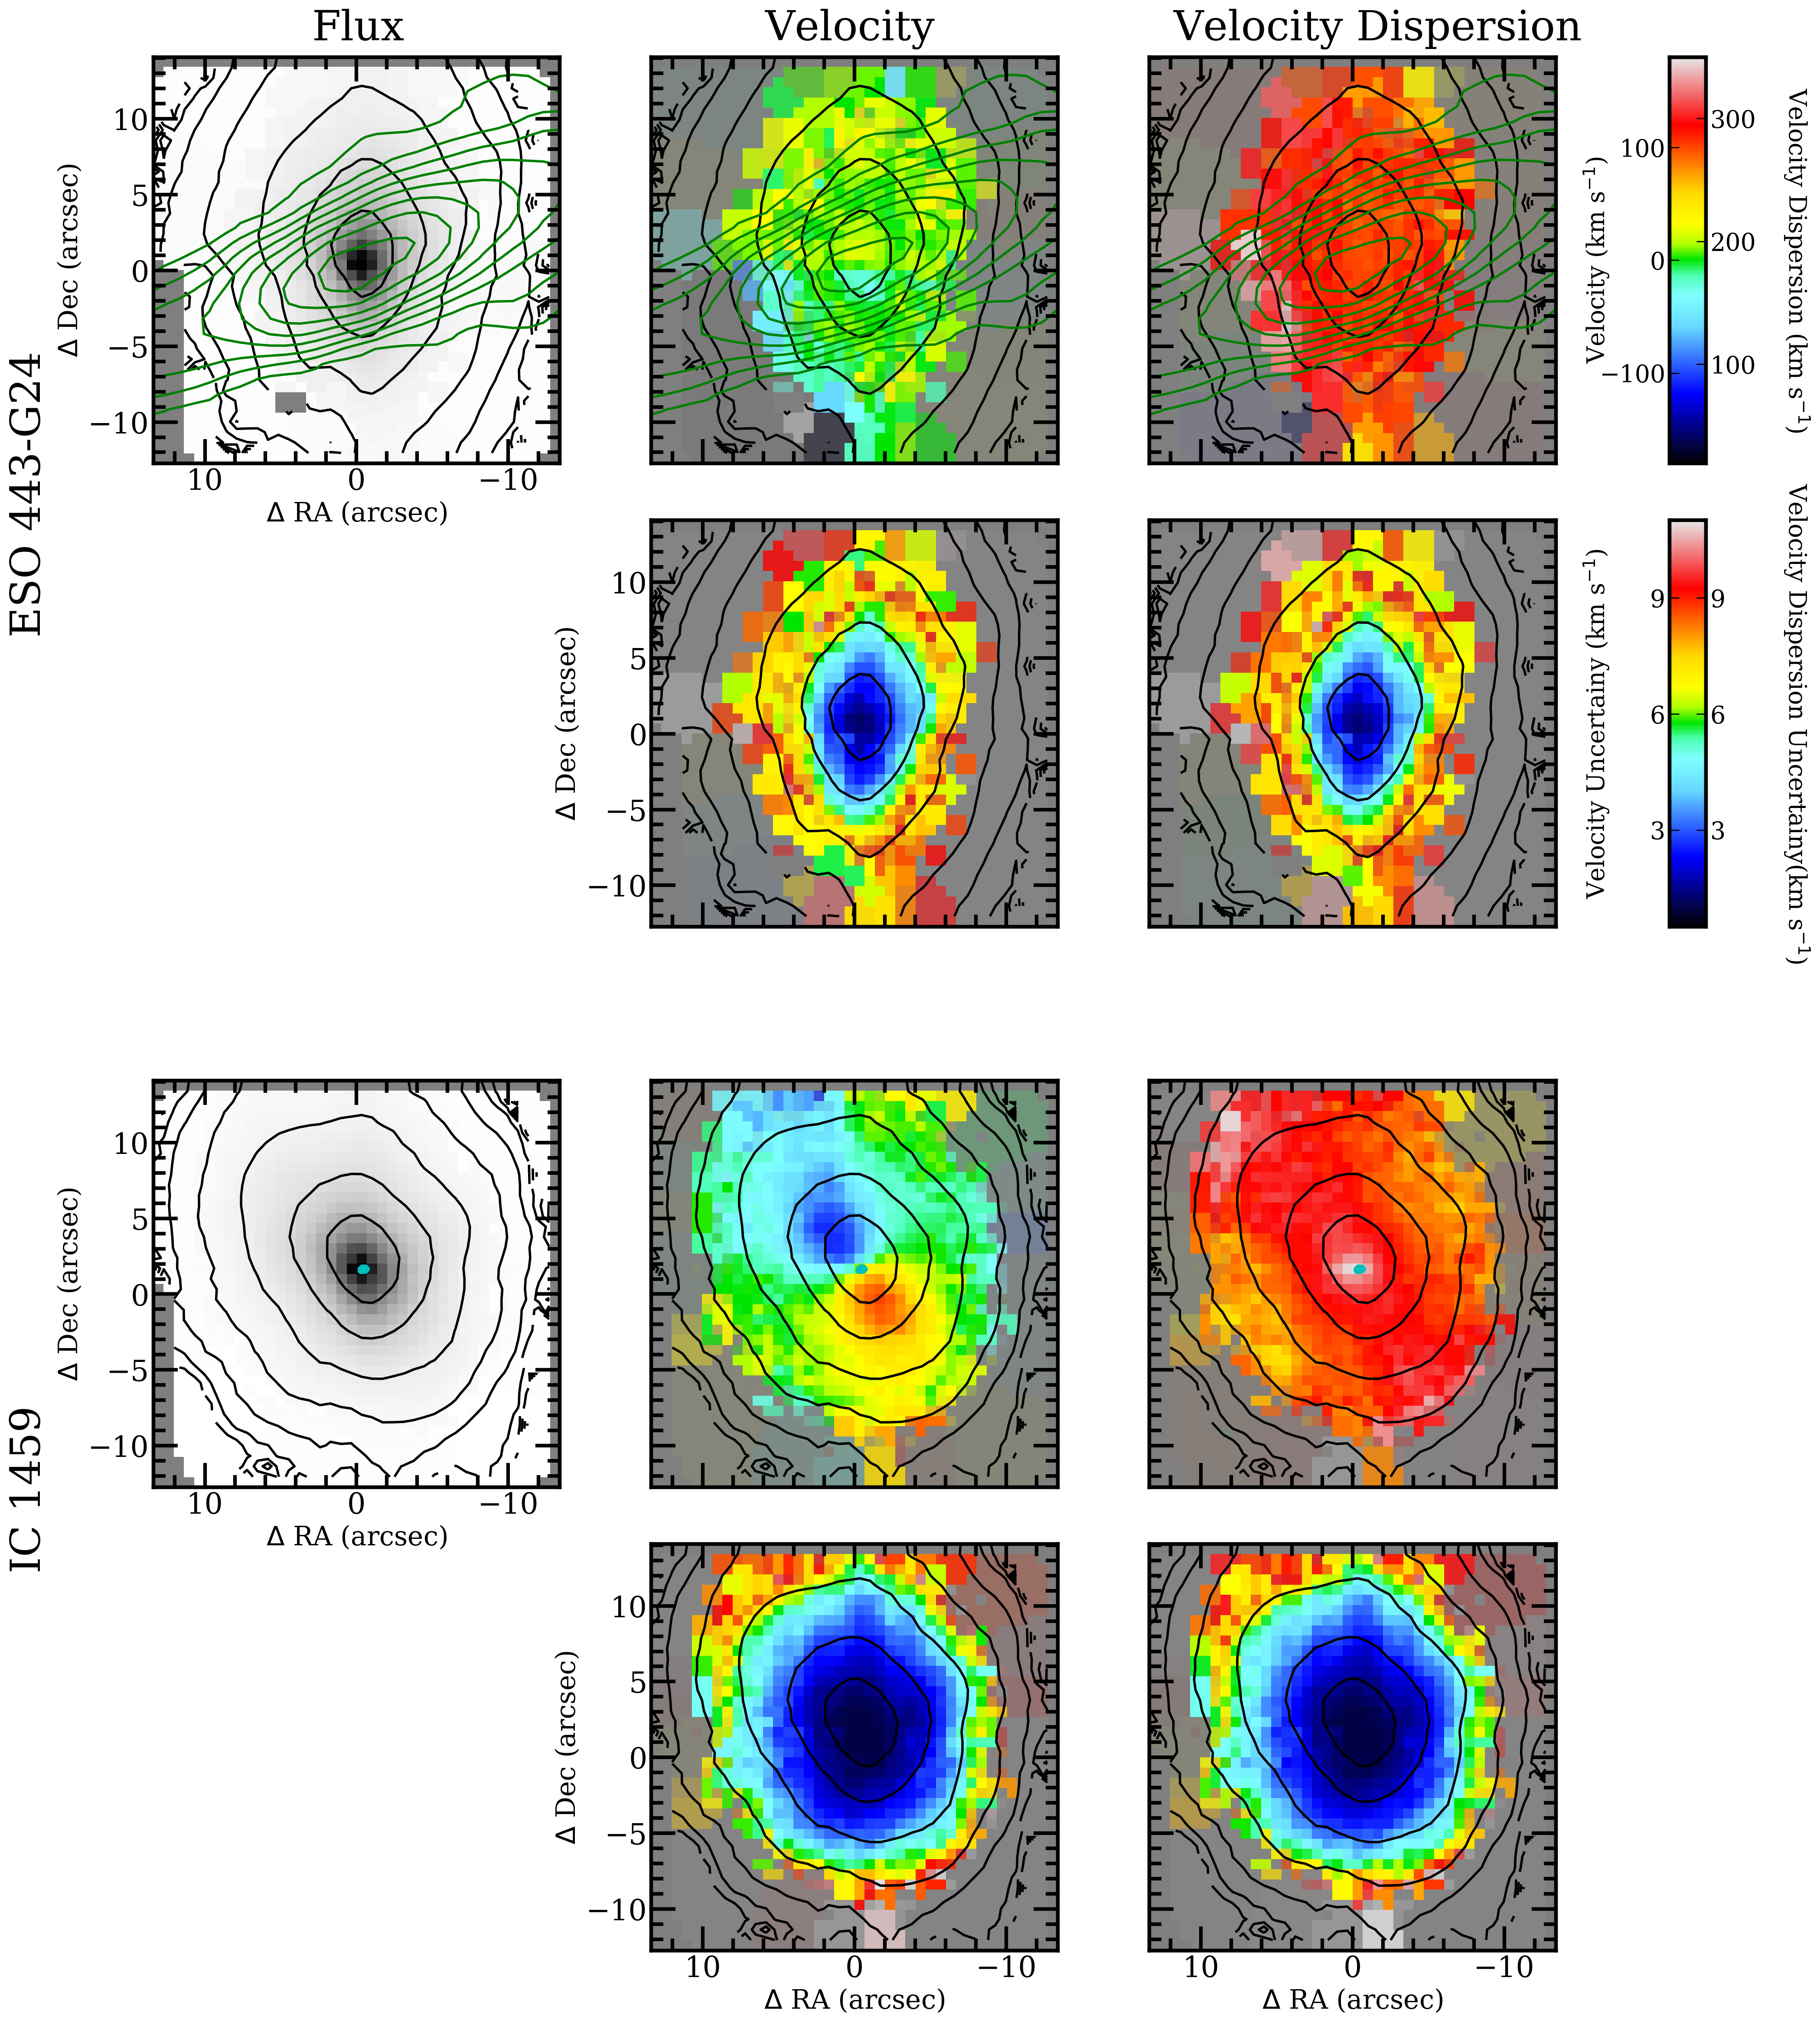
\includegraphics[height=0.62\textheight]{chapter4/vimos/kin1.png}
			\caption[VIMOS stellar kinematic maps]{VIMOS stellar kinematic maps. Left to right: flux (image), mean velocity and velocity dispersion. Top to bottom: ESO 443-G24 and IC 1459. Alternate rows show a given parameter its associated uncertainty. Flux contours (isophotes) are shown in black, \ce{^{12}CO(2-1)} contours from ALMA in cyan and radio continuum contours from VLA in green. The radio band displayed depends on the data available in the archive and which images had a similar resolution and scales. Limits on the colour scale are: mean velocity maps -180 to 180\,$\mathrm{km \, s^{-1}}$, mean velocity uncertainty 1 to 11\,$\mathrm{km \, s^{-1}}$, velocity dispersion 35 to 350\,$\mathrm{km \, s^{-1}}$ and velocity dispersion uncertainty 1 to 11\,$\mathrm{km \, s^{-1}}$.} 
			\label{fig:VIMOS_stellar}
		\end{figure}
		\begin{figure}
			\centering
			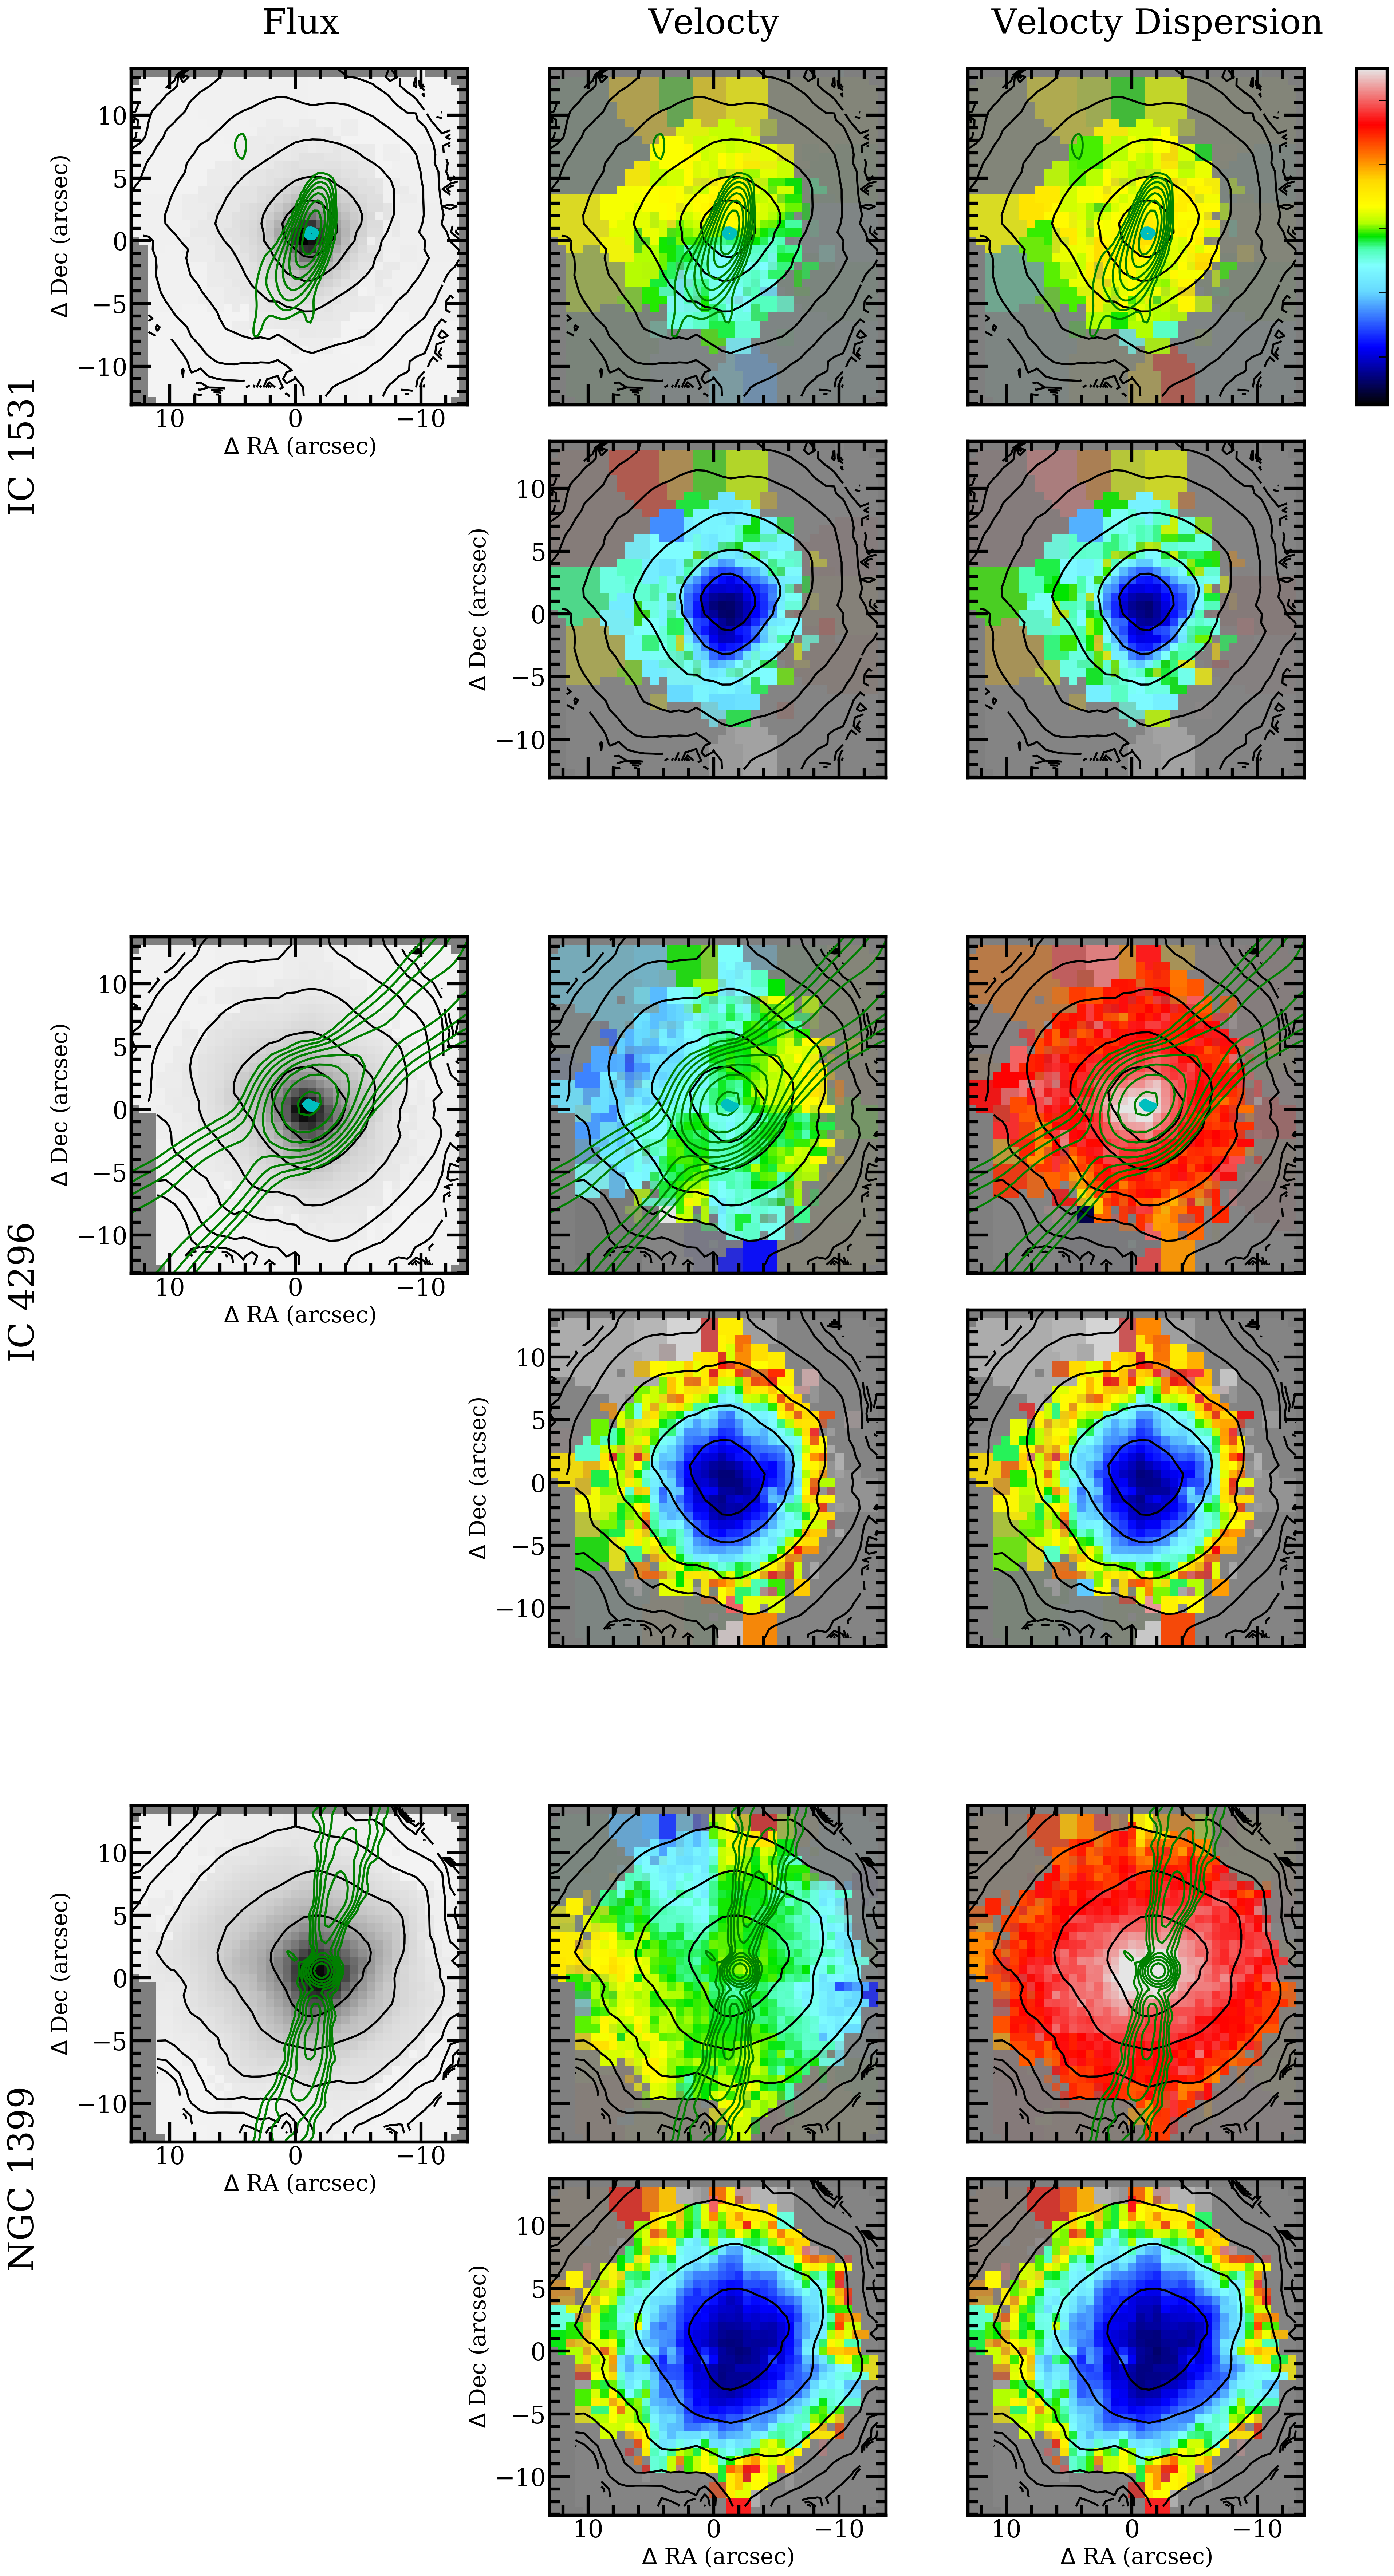
\includegraphics[height=0.94\textheight]{chapter4/vimos/kin2.png}
			\contcaption{\textit{Continued.}}
		\end{figure}
		\begin{figure}
			\centering
			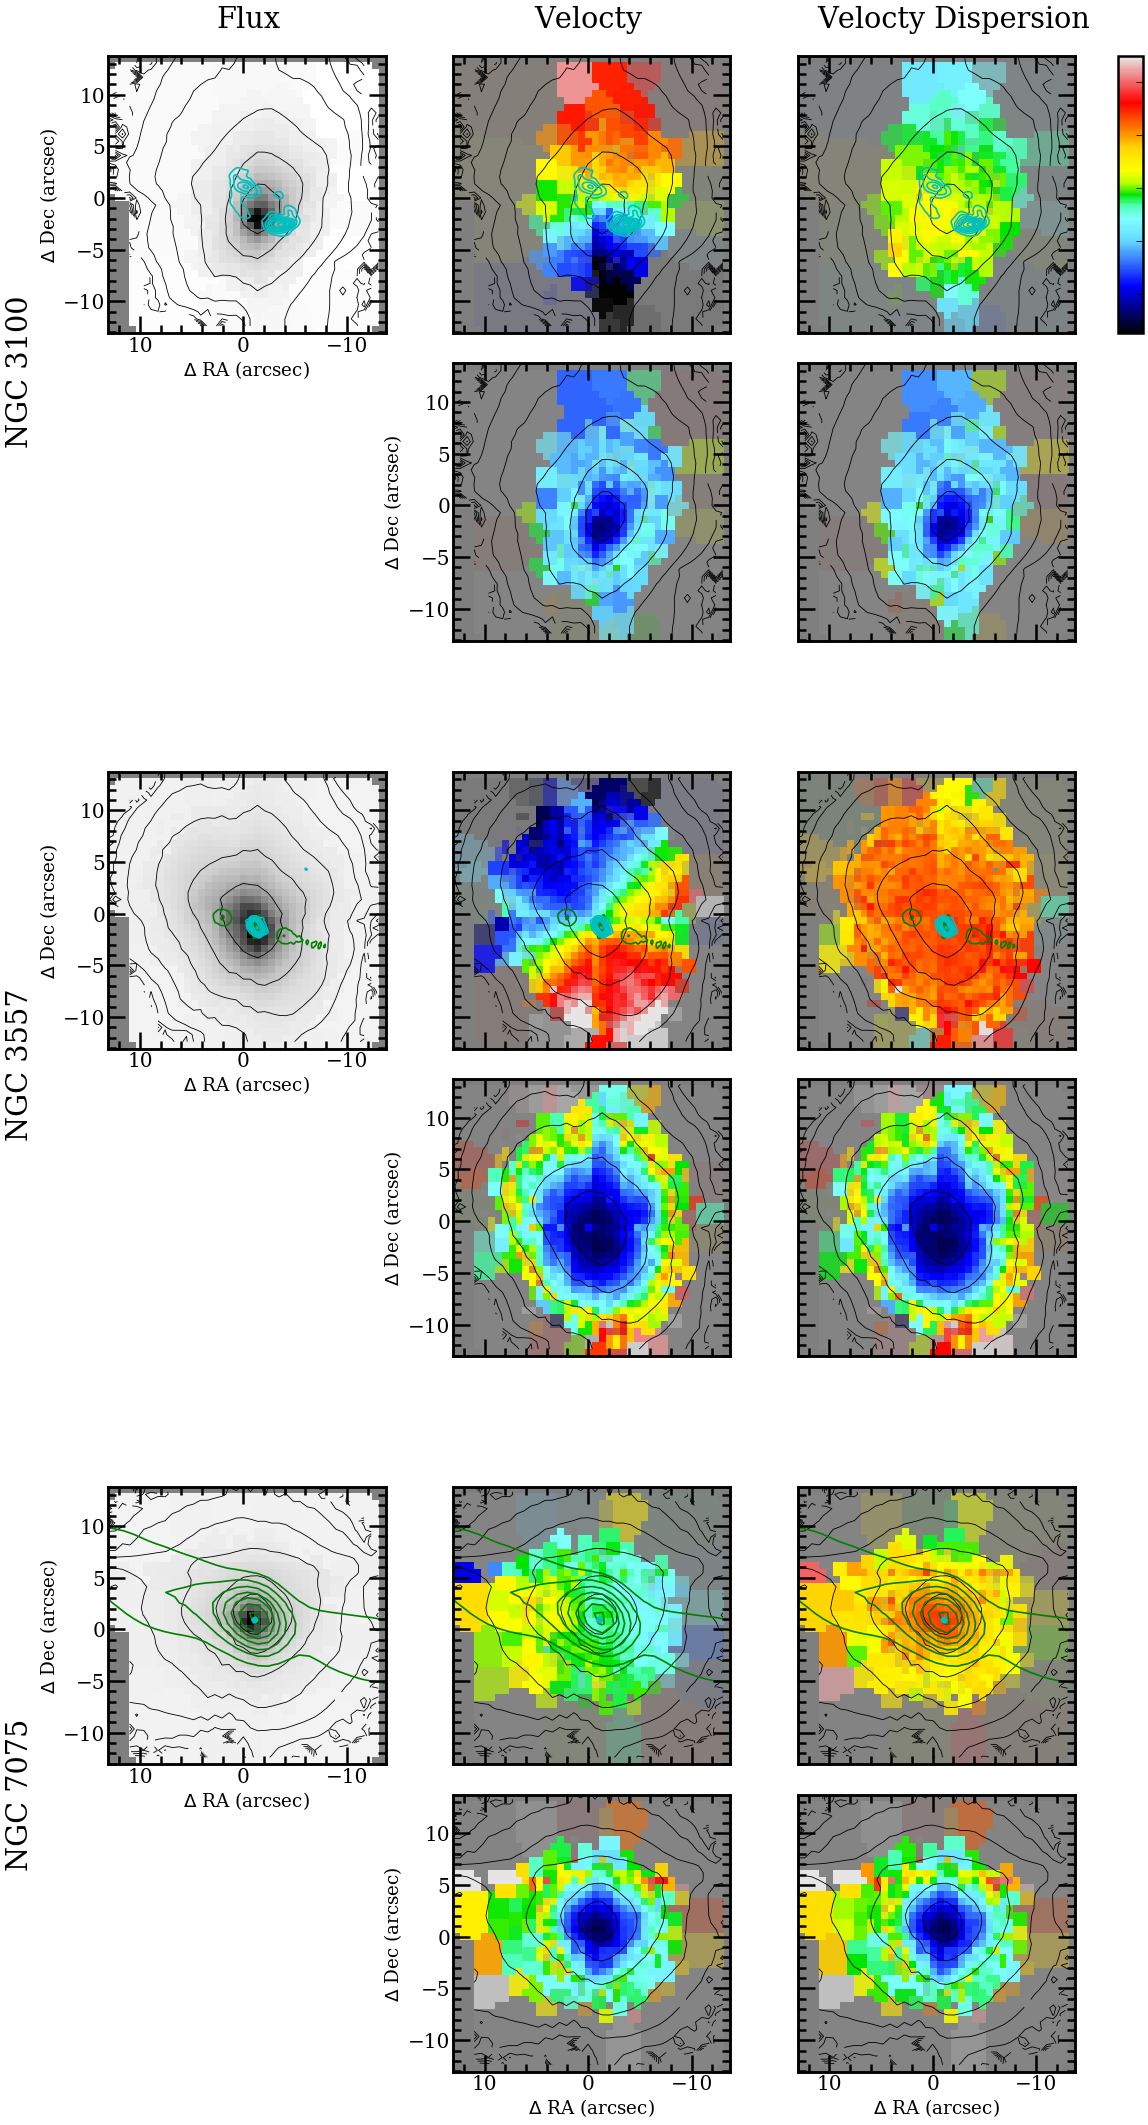
\includegraphics[height=0.94\textheight]{chapter4/vimos/kin3.png}
			\contcaption{\textit{Continued.}}
		\end{figure}
		\begin{figure}
			\centering
			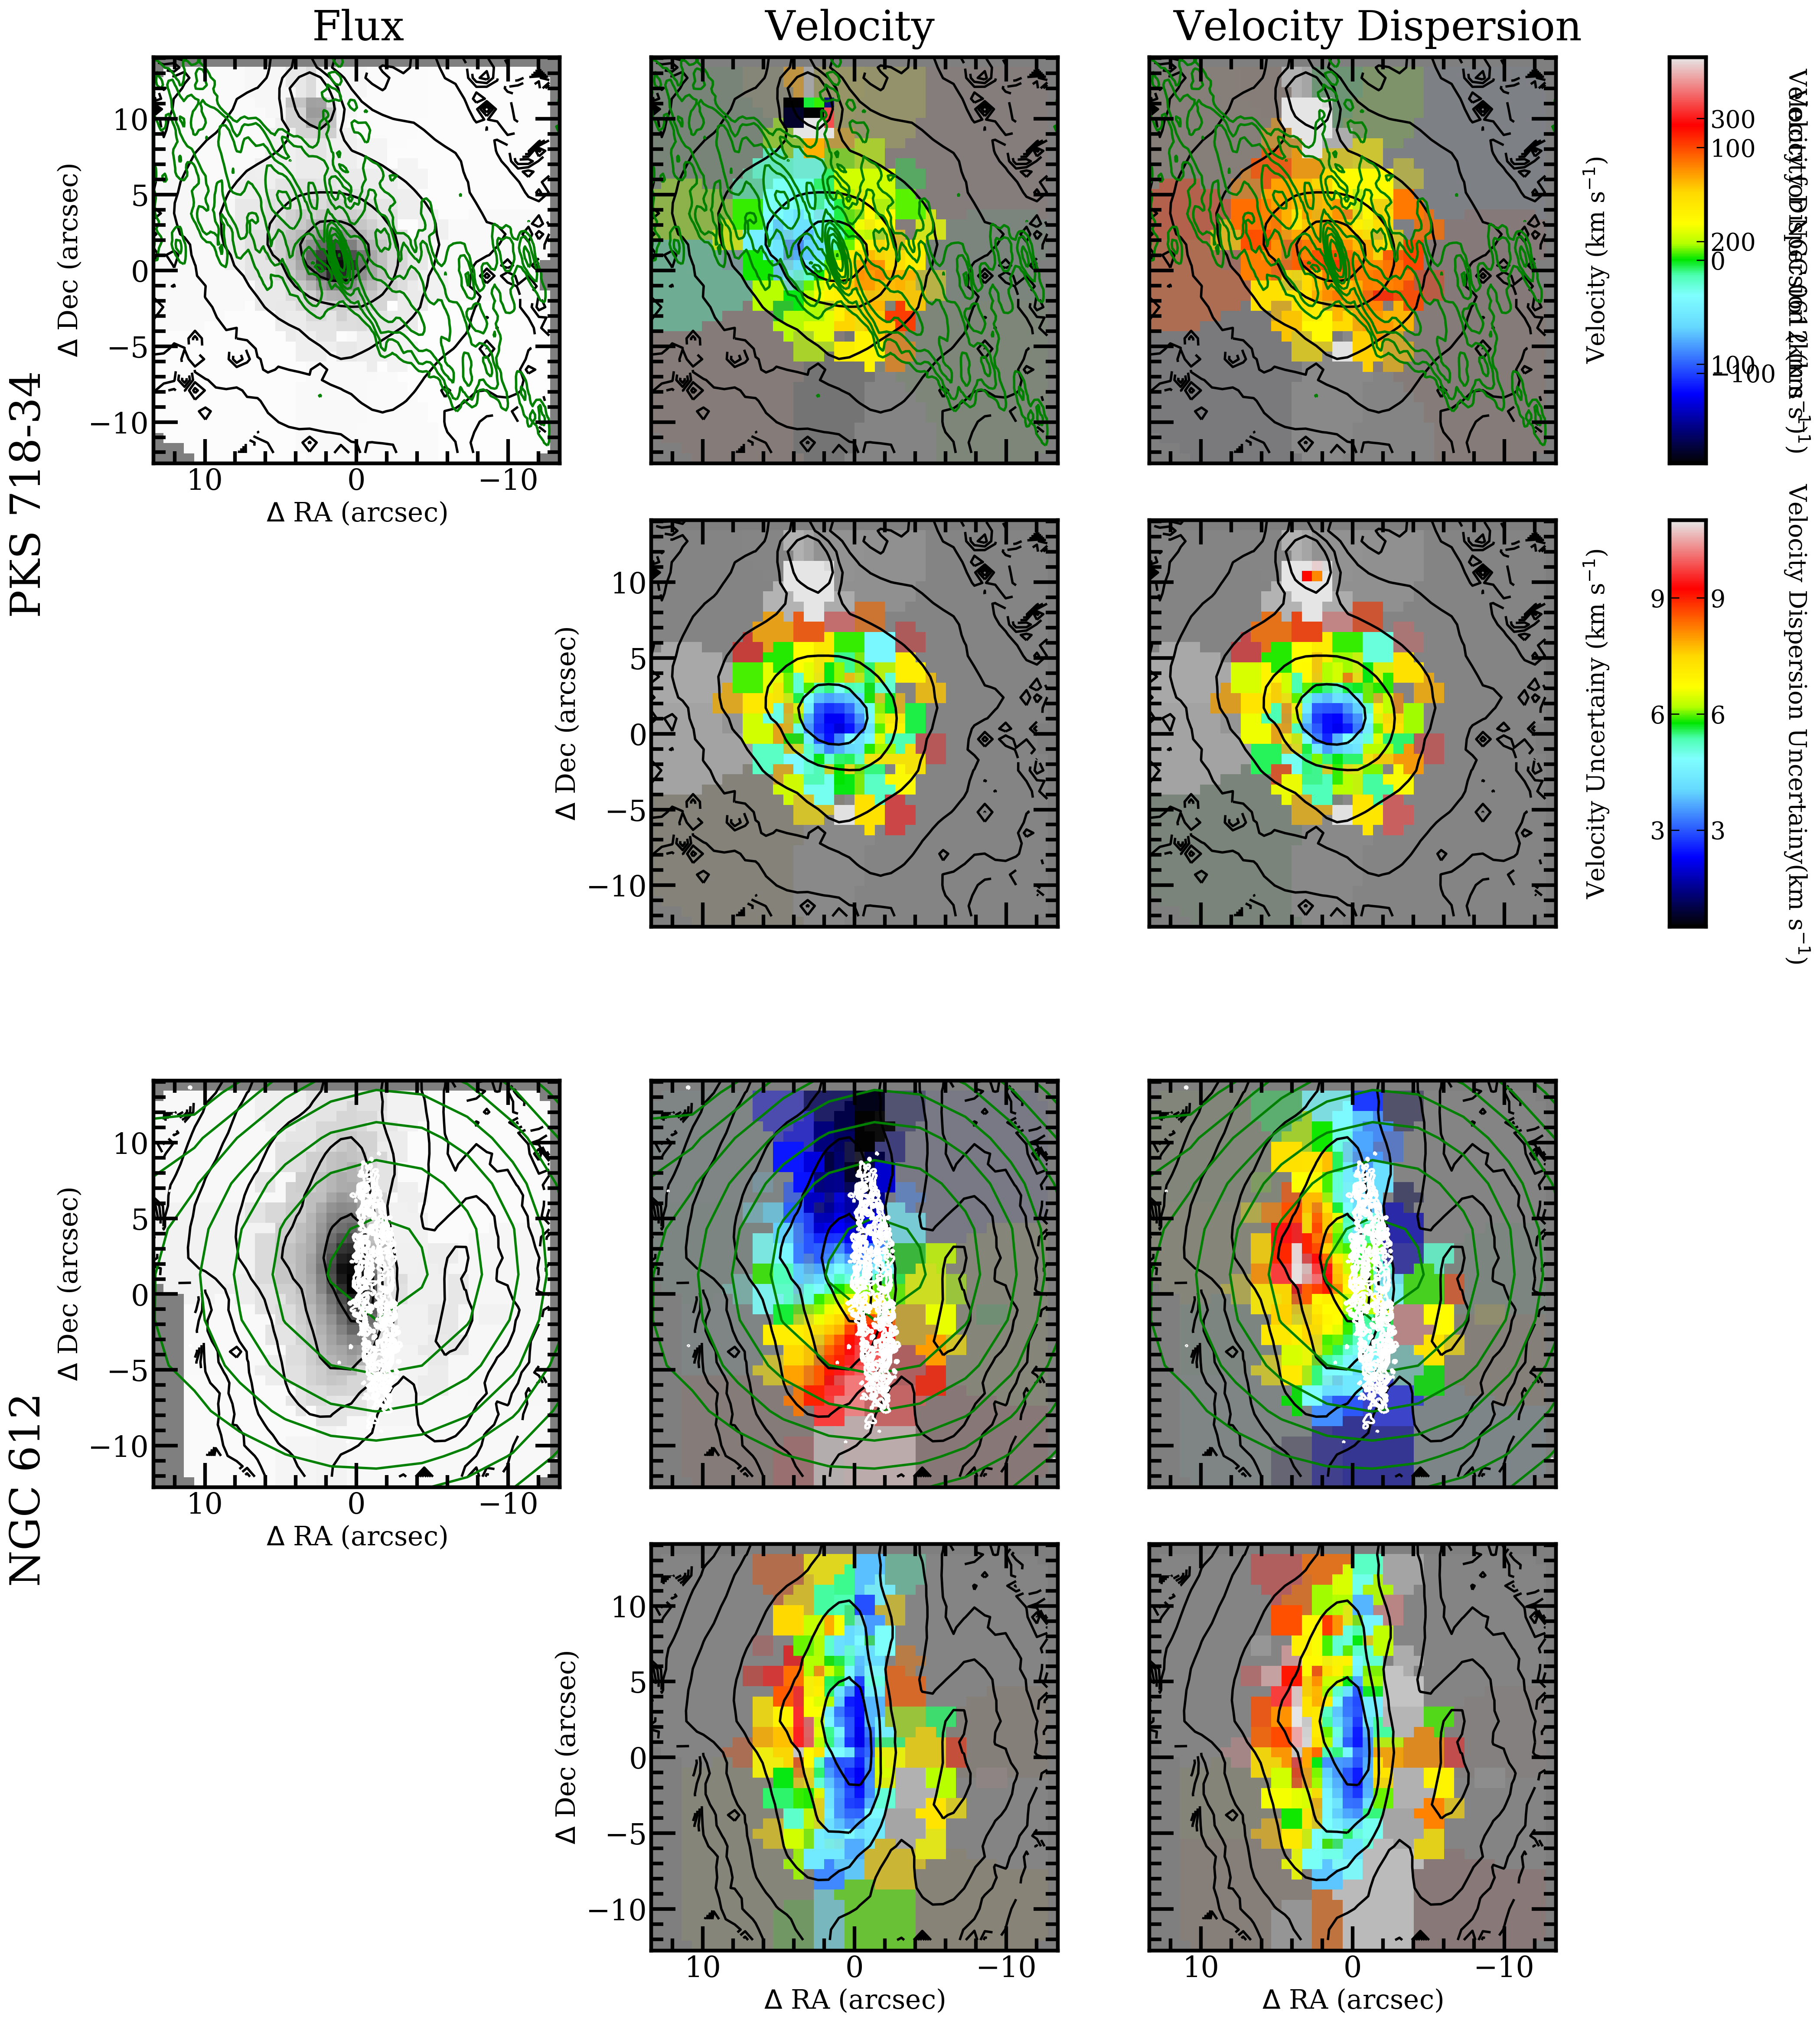
\includegraphics[height=0.62\textheight]{chapter4/vimos/kin4.png}
			\contcaption{\textit{Continued.} The colour scale for the mean velocity map of NGC 612 only is $-322$ to $322 \, \mathrm{km \, s^{-1}}$.}
		\end{figure}

		\begin{figure}
			\centering
			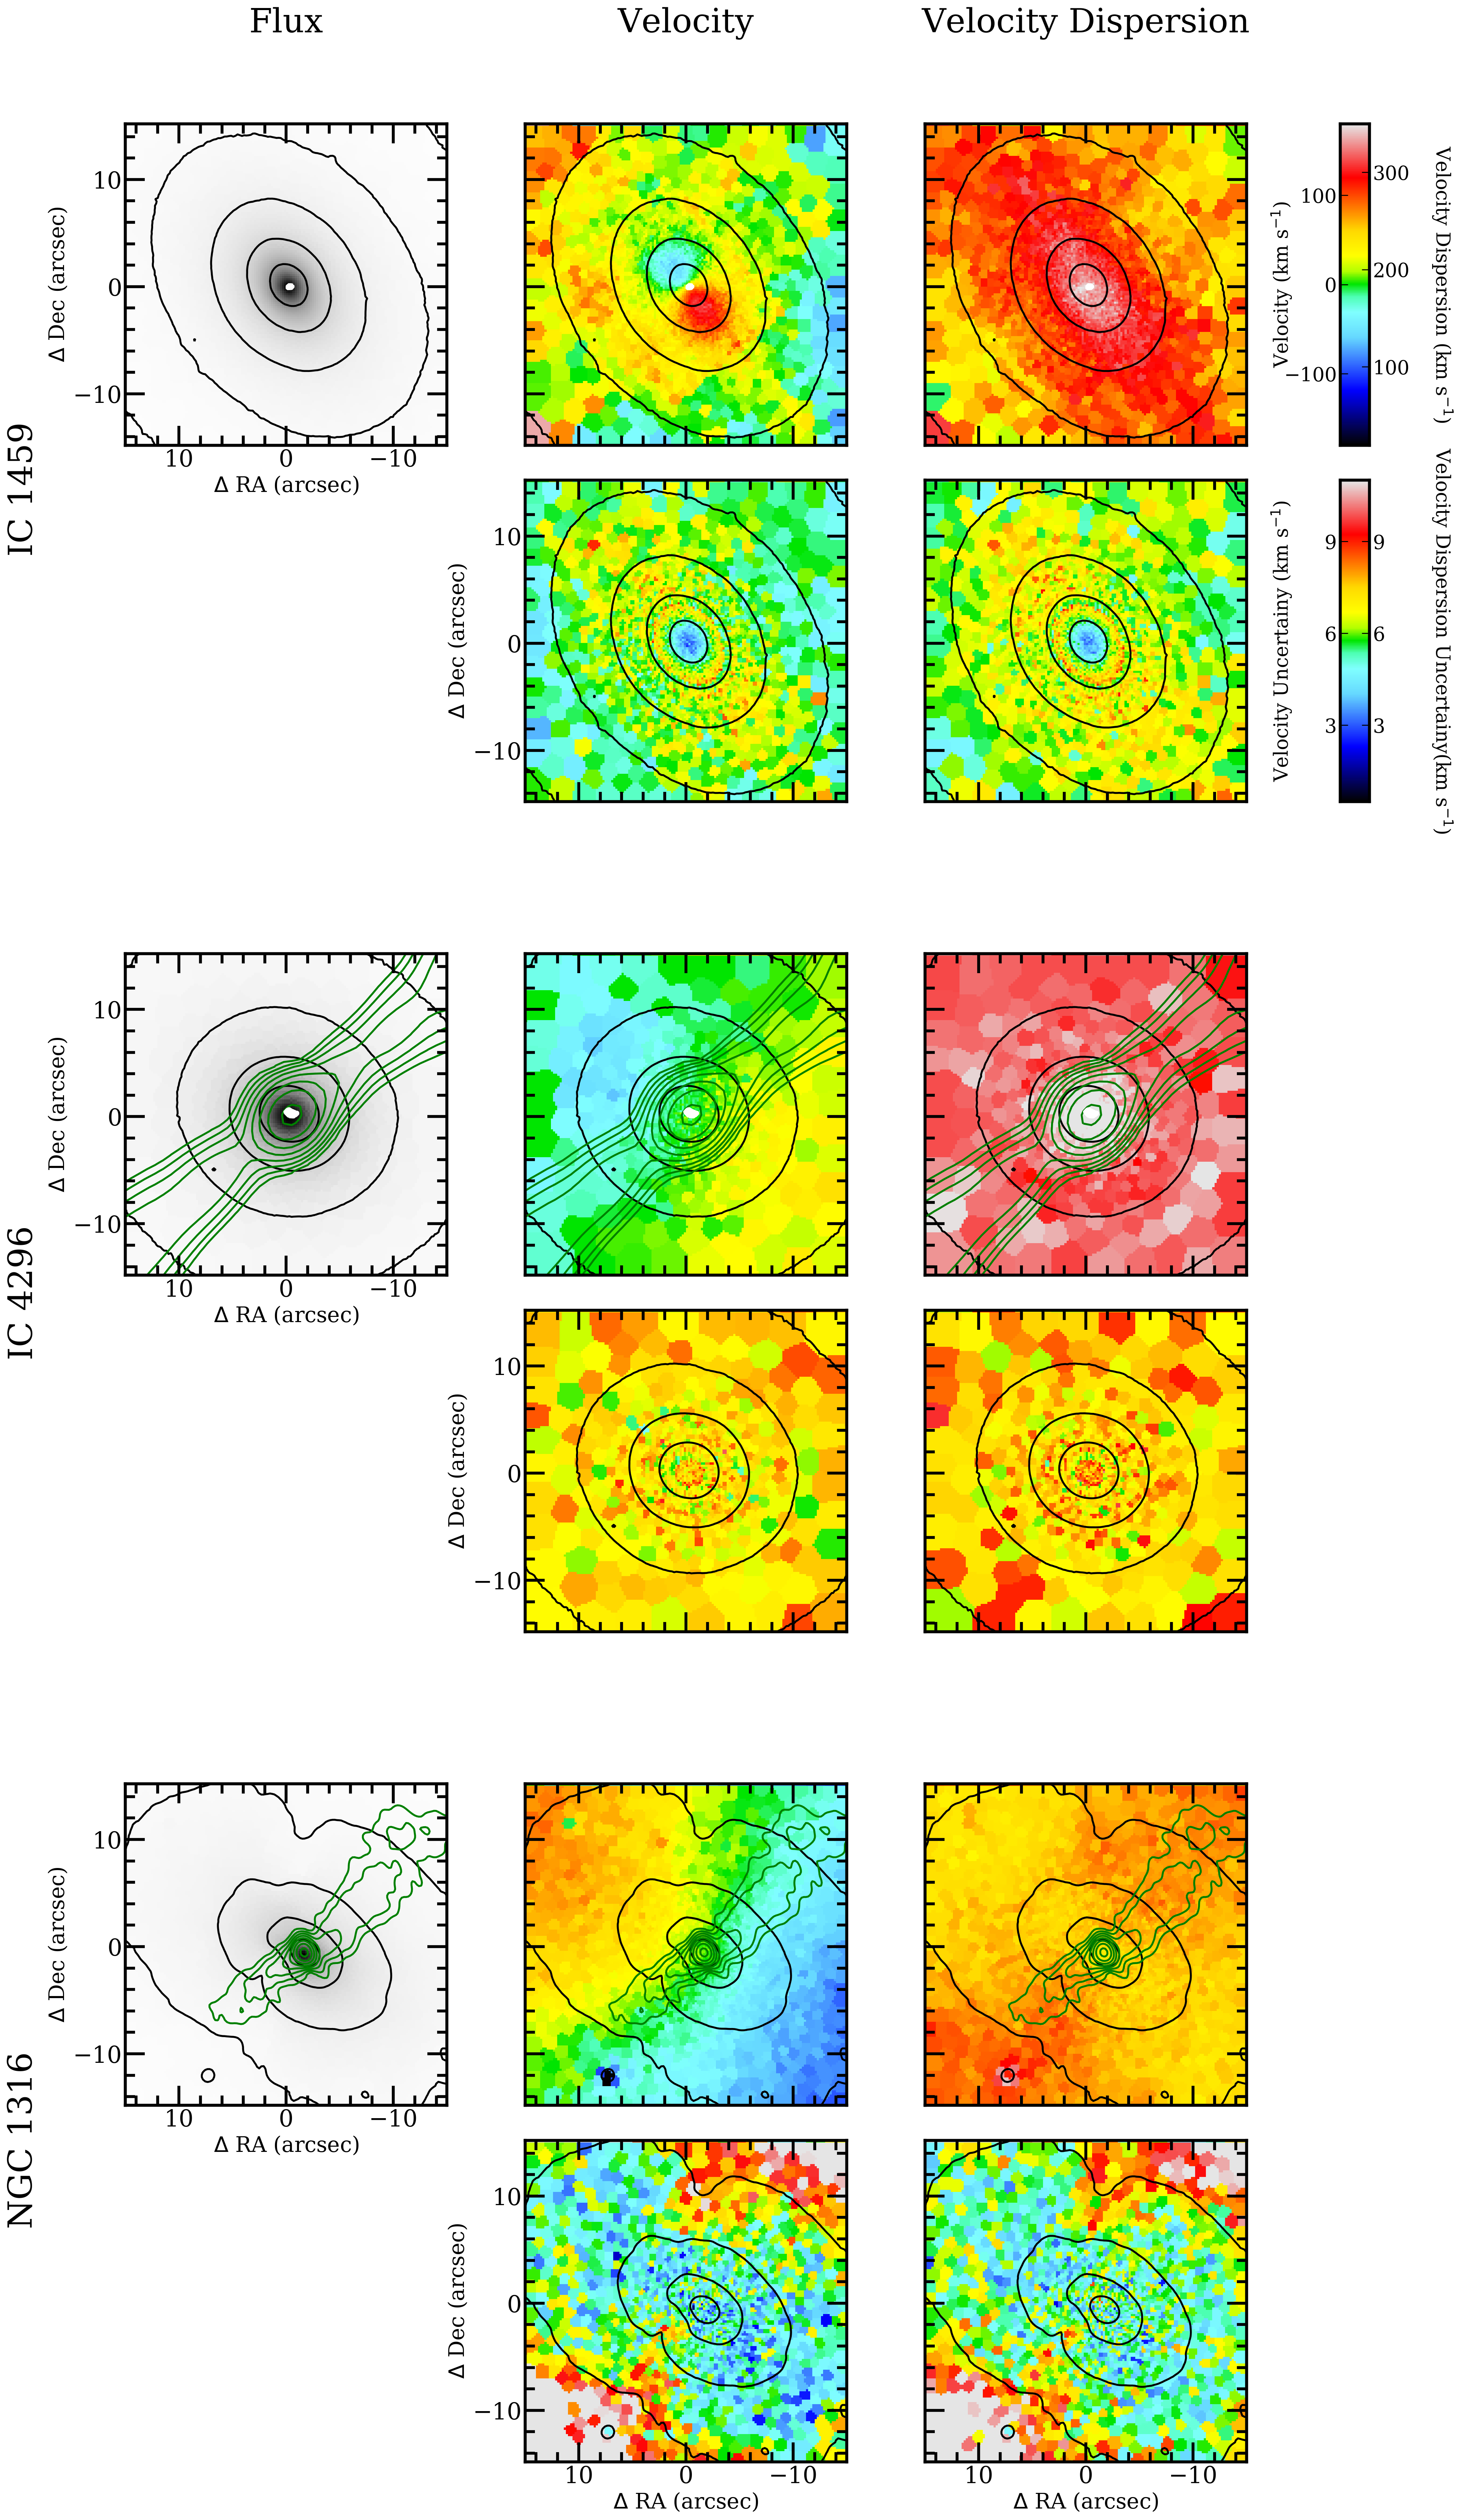
\includegraphics[height=0.62\textheight]{chapter4/muse/kin1.png}
			\caption[MUSE stellar kinematic maps]{As in Figure \ref{fig:VIMOS_stellar} but for the MUSE stellar kinematic maps.}
			\label{fig:MUSE_stellar}
		\end{figure}
		\begin{figure}
			\centering
			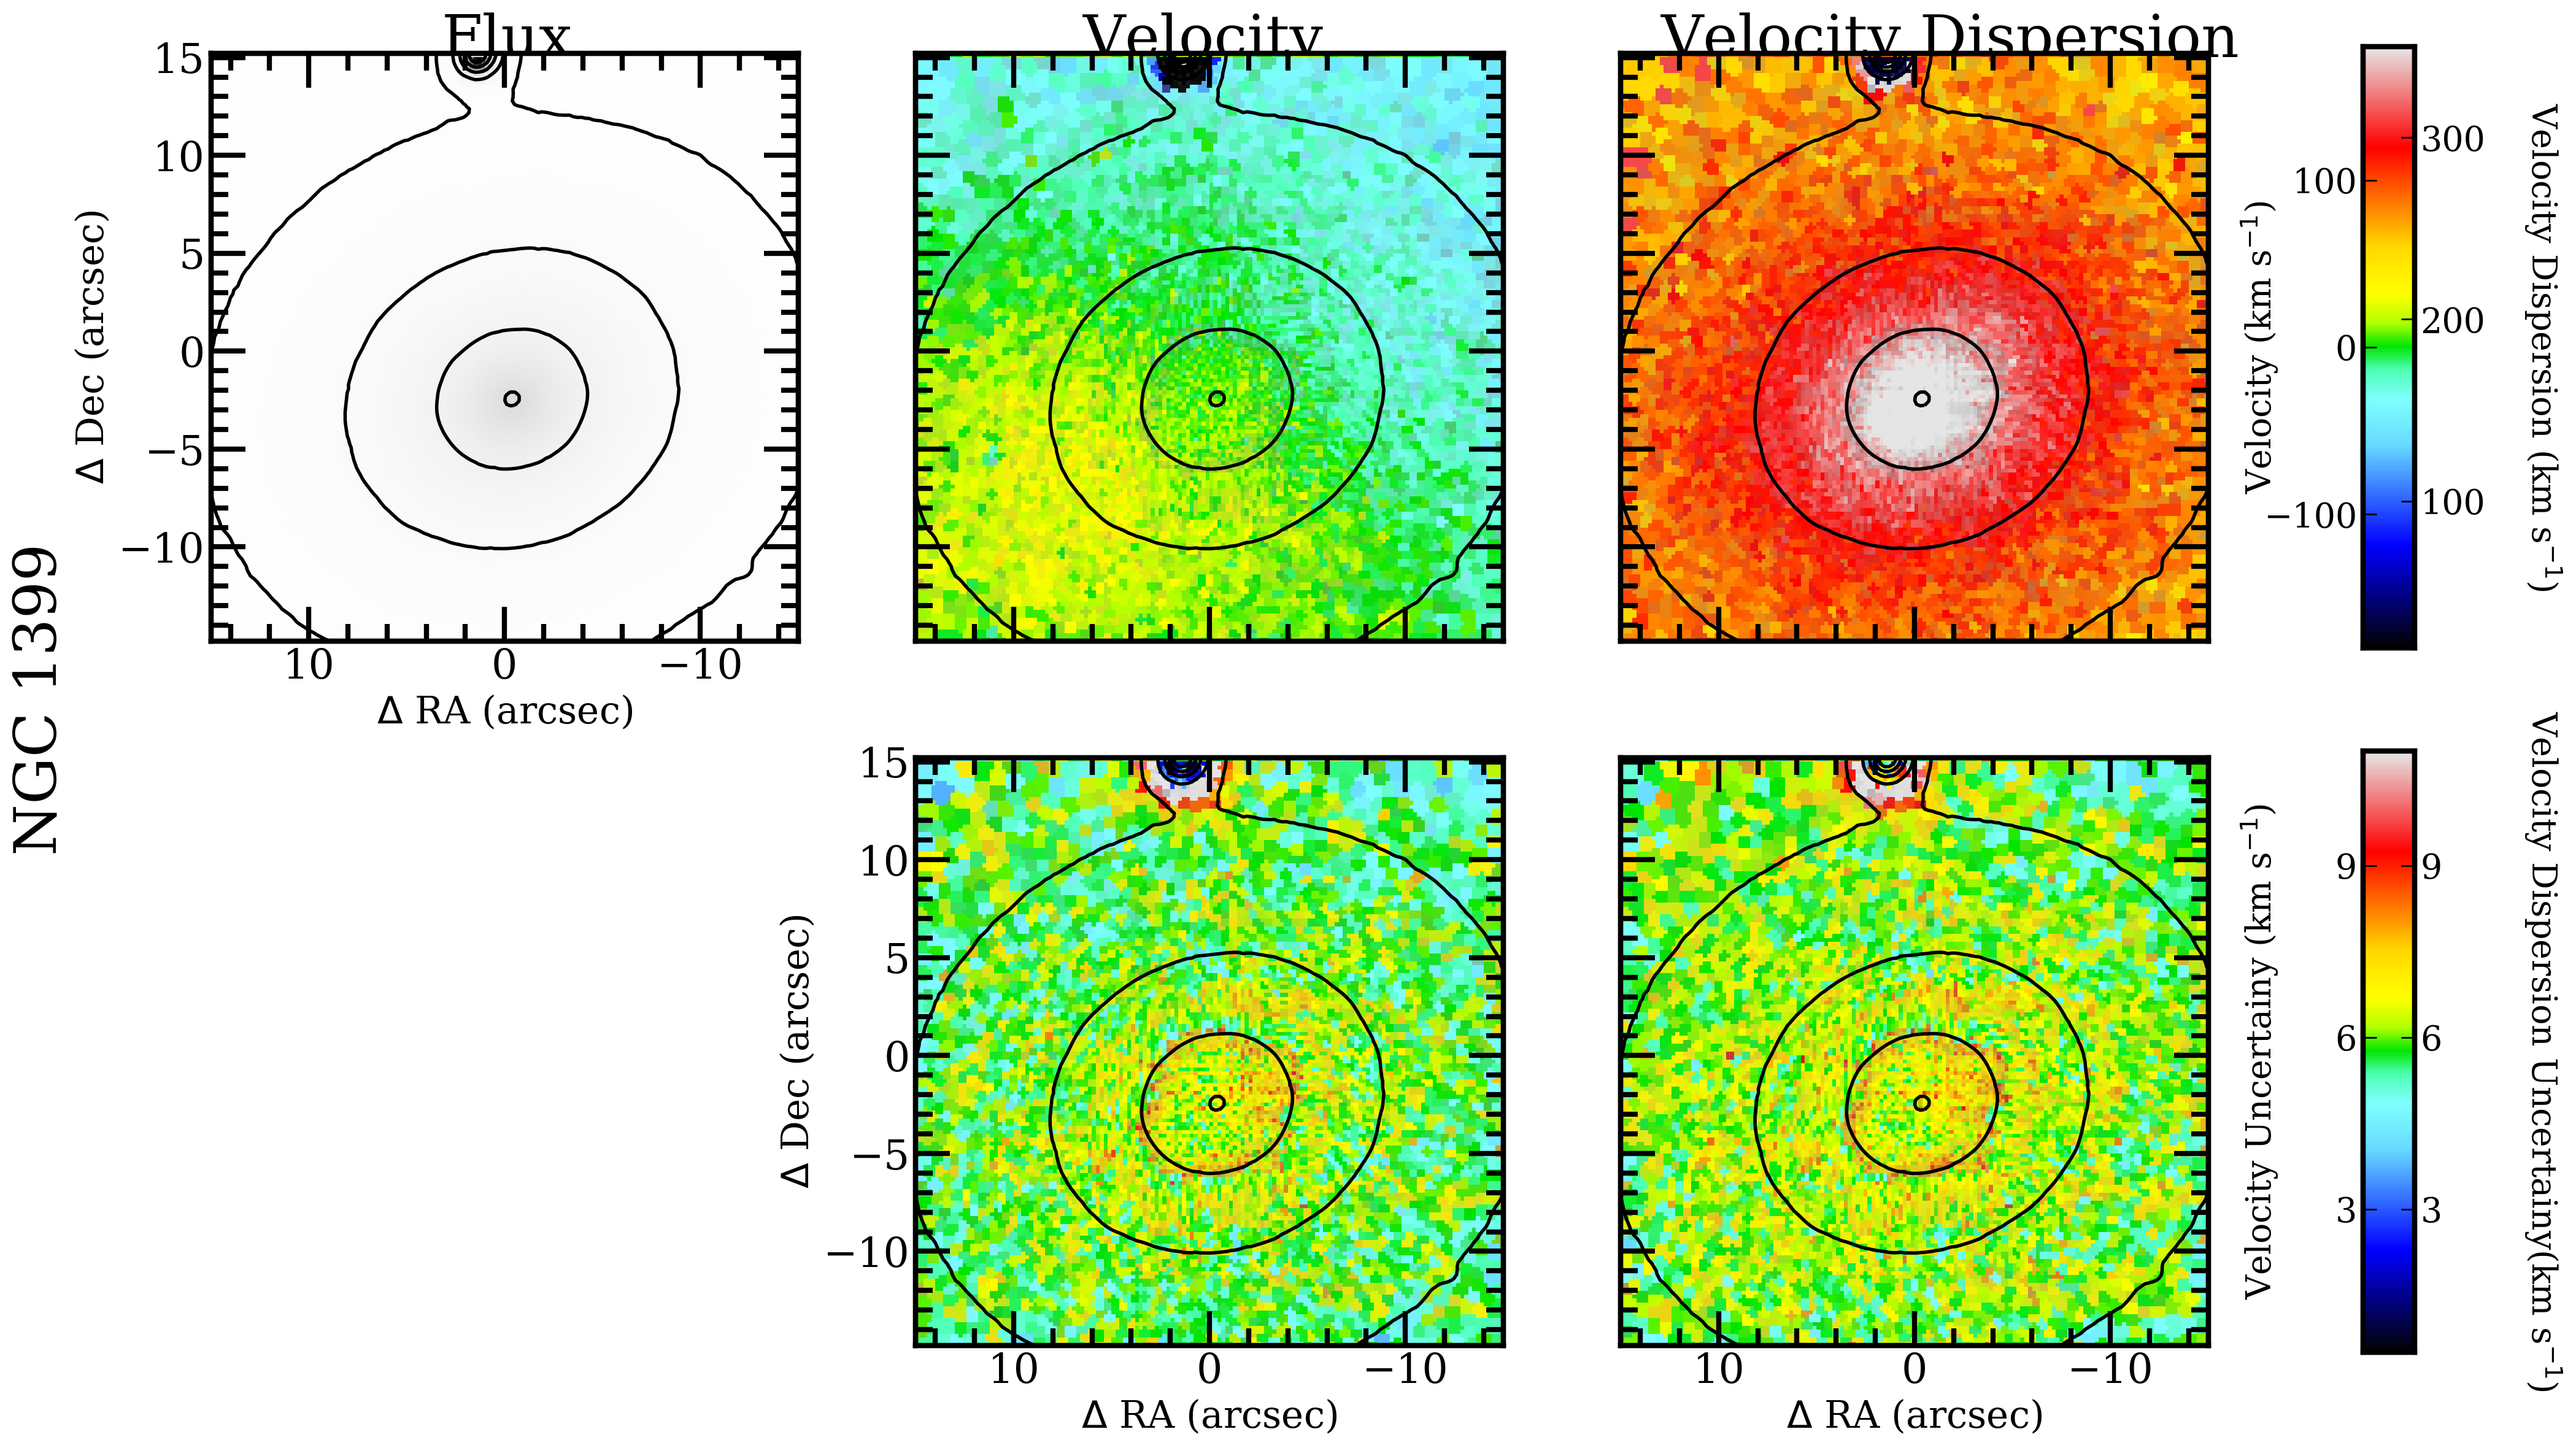
\includegraphics[height=0.62\textheight]{chapter4/muse/kin2.png}
			\contcaption{\textit{Continued.}}
		\end{figure}



		\begin{table}
			\centering
		\begin{threeparttable}
			\caption{Kinematic classifications}
			\label{tab:classify}
			\begin{tabular}{l c c c c c c c}
				\hline
				\hline
				Galaxy		& $\lambda_\mathrm{R_e}$ & $\epsilon_\mathrm{e}$  & $\Gamma_\text{kin}$ (deg) & FR/SR 	& RR/NRR 	& Feature & Group 	\\
				\hline 
				ESO 443-G024 & 0.048 & 0.35 & $-18\pm\leavevmode\phantom{0}2$	& SR & NRR & KDC & c \\
				IC 1459 	& 0.125 & 0.24 & \leavevmode\phantom{0}$-3\pm\leavevmode\phantom{0}1$ & SR & NRR & KDC & c \\
				IC 1531 	& 0.101 & 0.08 & $-54\pm25$	& FR & NRR & LV & a \\
				IC 4296		& 0.034 & 0.03 & \leavevmode\phantom{$-0$}$8\pm12$ & SR &\leavevmode\phantom{N}RR & -- & e \\
				NGC 612 	& 0.655 & 0.36 & \leavevmode\phantom{$-$}$12\pm\leavevmode\phantom{0}6$	& FR &\leavevmode\phantom{N}RR & -- & e \\
				NGC 1316 	& 0.100 & 0.39 & \leavevmode\phantom{$-0$}$6\pm\leavevmode\phantom{0}2$ & FR & NRR & -- & f \\
				NGC 1399 	& 0.090 & 0.12 & $-74\pm\leavevmode\phantom{0}5$ & SR & NRR & LV & a \\
				NGC 3100 	& 0.354 & 0.24 & \leavevmode\phantom{0}$-8\pm\leavevmode\phantom{0}2$ & FR &\leavevmode\phantom{N}RR & -- & e \\
				NGC 3557 	& 0.312 & 0.20 & \leavevmode\phantom{$-$}$16\pm\leavevmode\phantom{0}5$ & FR &\leavevmode\phantom{N}RR & -- & e\\
				NGC 7075 	& 0.068 & 0.04 & \leavevmode\phantom{$-$}$36\pm50$ & SR & NRR & -- & b \\
				PKS 718-34  & 0.159 & 0.17 & \leavevmode\phantom{$-$}$15\pm25$ & FR & NRR & KDC$^\text{a}$ & b\\
				\hline
				\hline
			\end{tabular}
			\begin{tablenotes}
			\footnotesize
			\note $^\text{a}$ tentative classification. A higher signal-to-noise ratio (S/N) in the outer regions of the field of view is required for confirmation.
			\item Col.\,1: Galaxy name; col.\,2: $\lambda_\mathrm{R}$ evaluated at $R_\mathrm{e}$; col.\,3: Ellipticity at $R_\mathrm{e}$; col.\,4: Misalignment between the kinematic and photometric position angles; col.\,5: Fast-/slow-rotator (FR/SR) classification; col.\,6: Regular-rotator (RR) or non-regular-rotator (NRR); col.\,7: Kinematic features; col.\,8: Kinematic group.
			\end{tablenotes}
		\end{threeparttable}
		\end{table}

		The stellar kinematics of the sample galaxies are classified according to the regular rotator/non-regular rotator (RR/NRR) categories of \citet{Krajnovic2011}, with the results listed in Col.\,6 of Table \ref{tab:classify}. Here and hereafter, where MUSE datacubes exist their derived properties are quoted. Otherwise the values are derived from the VIMOS datacubes. We find 4/11 of our sample galaxies are regular rotators.

		In addition to this, we attempt to identify the kinematic features defined by \citet{Krajnovic2011} in an algorithmic way. However, the artifacts from the VIMOS quadrants (see Section \ref{subsec:VIMOSartifacts}) confuse ellipse fitting algorithms so only maps derived from the MUSE data are classified in this way; kinematic features in maps derived from the VIMOS data are identified by eye. These classification are listed in Col.\,7 of Table \ref{tab:classify} and corresponding kinematic group (see Table \ref{tab:KinGroups} and Fig.\,\ref{fig:EgSubstructure} for group definitions and examples) that a given galaxy belongs to is given is Col.\,8. We see 3 KDCs (although PKS 718-34 is only a tentative classification). 
% Comparisons. ^^^^


		\subsection{Ellipticity}
			\label{subsec:Ellipticity}
			Ellipticity is measured as the ellipticity of the best-fitting ellipse to the surface-brightness map with an mean radius, $R_\mathrm{m}$, of 1 effective radius, $R_\mathrm{e}$. Firstly the centre of the galaxy is found as the luminosity weighted centre using the \textsc{python} routine \textsc{find\_galaxy}, which is part of the \textsc{mge} package\footnote{http://www-astro.physics.ox.ac.uk/\~mxc/software/} by \citet{Cappellari2002}. This is then used as an input for the \textsc{IDL} routine \textsc{kinemetry}\footnote{http://davor.krajnovic.org/idl/} by \citet{krajnovic2006} which finds the best-fitting ellipses at a range of evenly spaced semi-major axes. This is achieved by performing harmonic expansion of maps along ellipses with a given semi-major axis and, when used for even moments (e.g. surface brightness, velocity dispersion, h$_4$ etc.), minimising the amplitude of the first and second harmonics. The results include the ellipticity, $epsilon$ and position angle $PA_\text{phot}$ of the best-fitting ellipse for each semi-major axis. The fit is repeated for increasing semi-major axis until $<$75\% of the ellipse is not contained within the field of view. 

			In reality, the VIMOS field of view does not always contain 1 $R_\mathrm{e}$. Where this is the case, we follow the method by \citet{Emsellem2007}, were $R_\mathrm{m}$ is redefined as $R_\mathrm{m} \equiv \sqrt{A_\mathrm{s}/\pi}$, where $A_\mathrm{s}$ is the area of the ellipse contained within the field of view. For a given galaxy, we fit ellipses as described above, up to $R_\mathrm{m} = R_\mathrm{max}$, where $A_\mathrm{s}$ reaches a maximum difference if 15\% to the area of the fitted ellipse, $A_\text{ellipse}$. The value $\epsilon_\mathrm{e}$, the ellipticity at 1 $R_\mathrm{e}$ or the $R_\text{max}$, whichever is smallest, is given in Table \ref{tab:classify}. 

		\subsection{Fast-/Slow-Rotator Classification}
			\label{subsec:FSRot}
			The specific angular momentum parameter $\lambda_R$ is evaluated at 1 $R_\mathrm{e}$ or $R_\text{max}$, whichever is smaller (as described for ellipticity in Section \ref{subsec:Ellipticity}), and is given in Table \ref{tab:classify}. This is plotted against the ellipticity, $\epsilon_\mathrm{e}$ (see Section \ref{subsec:Ellipticity}) in Fig.\,\ref{fig:lambdaR_ellip}. This plot shows the classification scheme of \citet{Cappellari2016} for the fast-/slow-rotator (FR/SR) categories (originally defined by \citealt{Emsellem2011}, but later refined by \citealt{Cappellari2016}; see Section \ref{sec:ETG}). This classification is given in Col.\,5 of Table \ref{tab:classify}.


			\begin{figure}
				\centering
				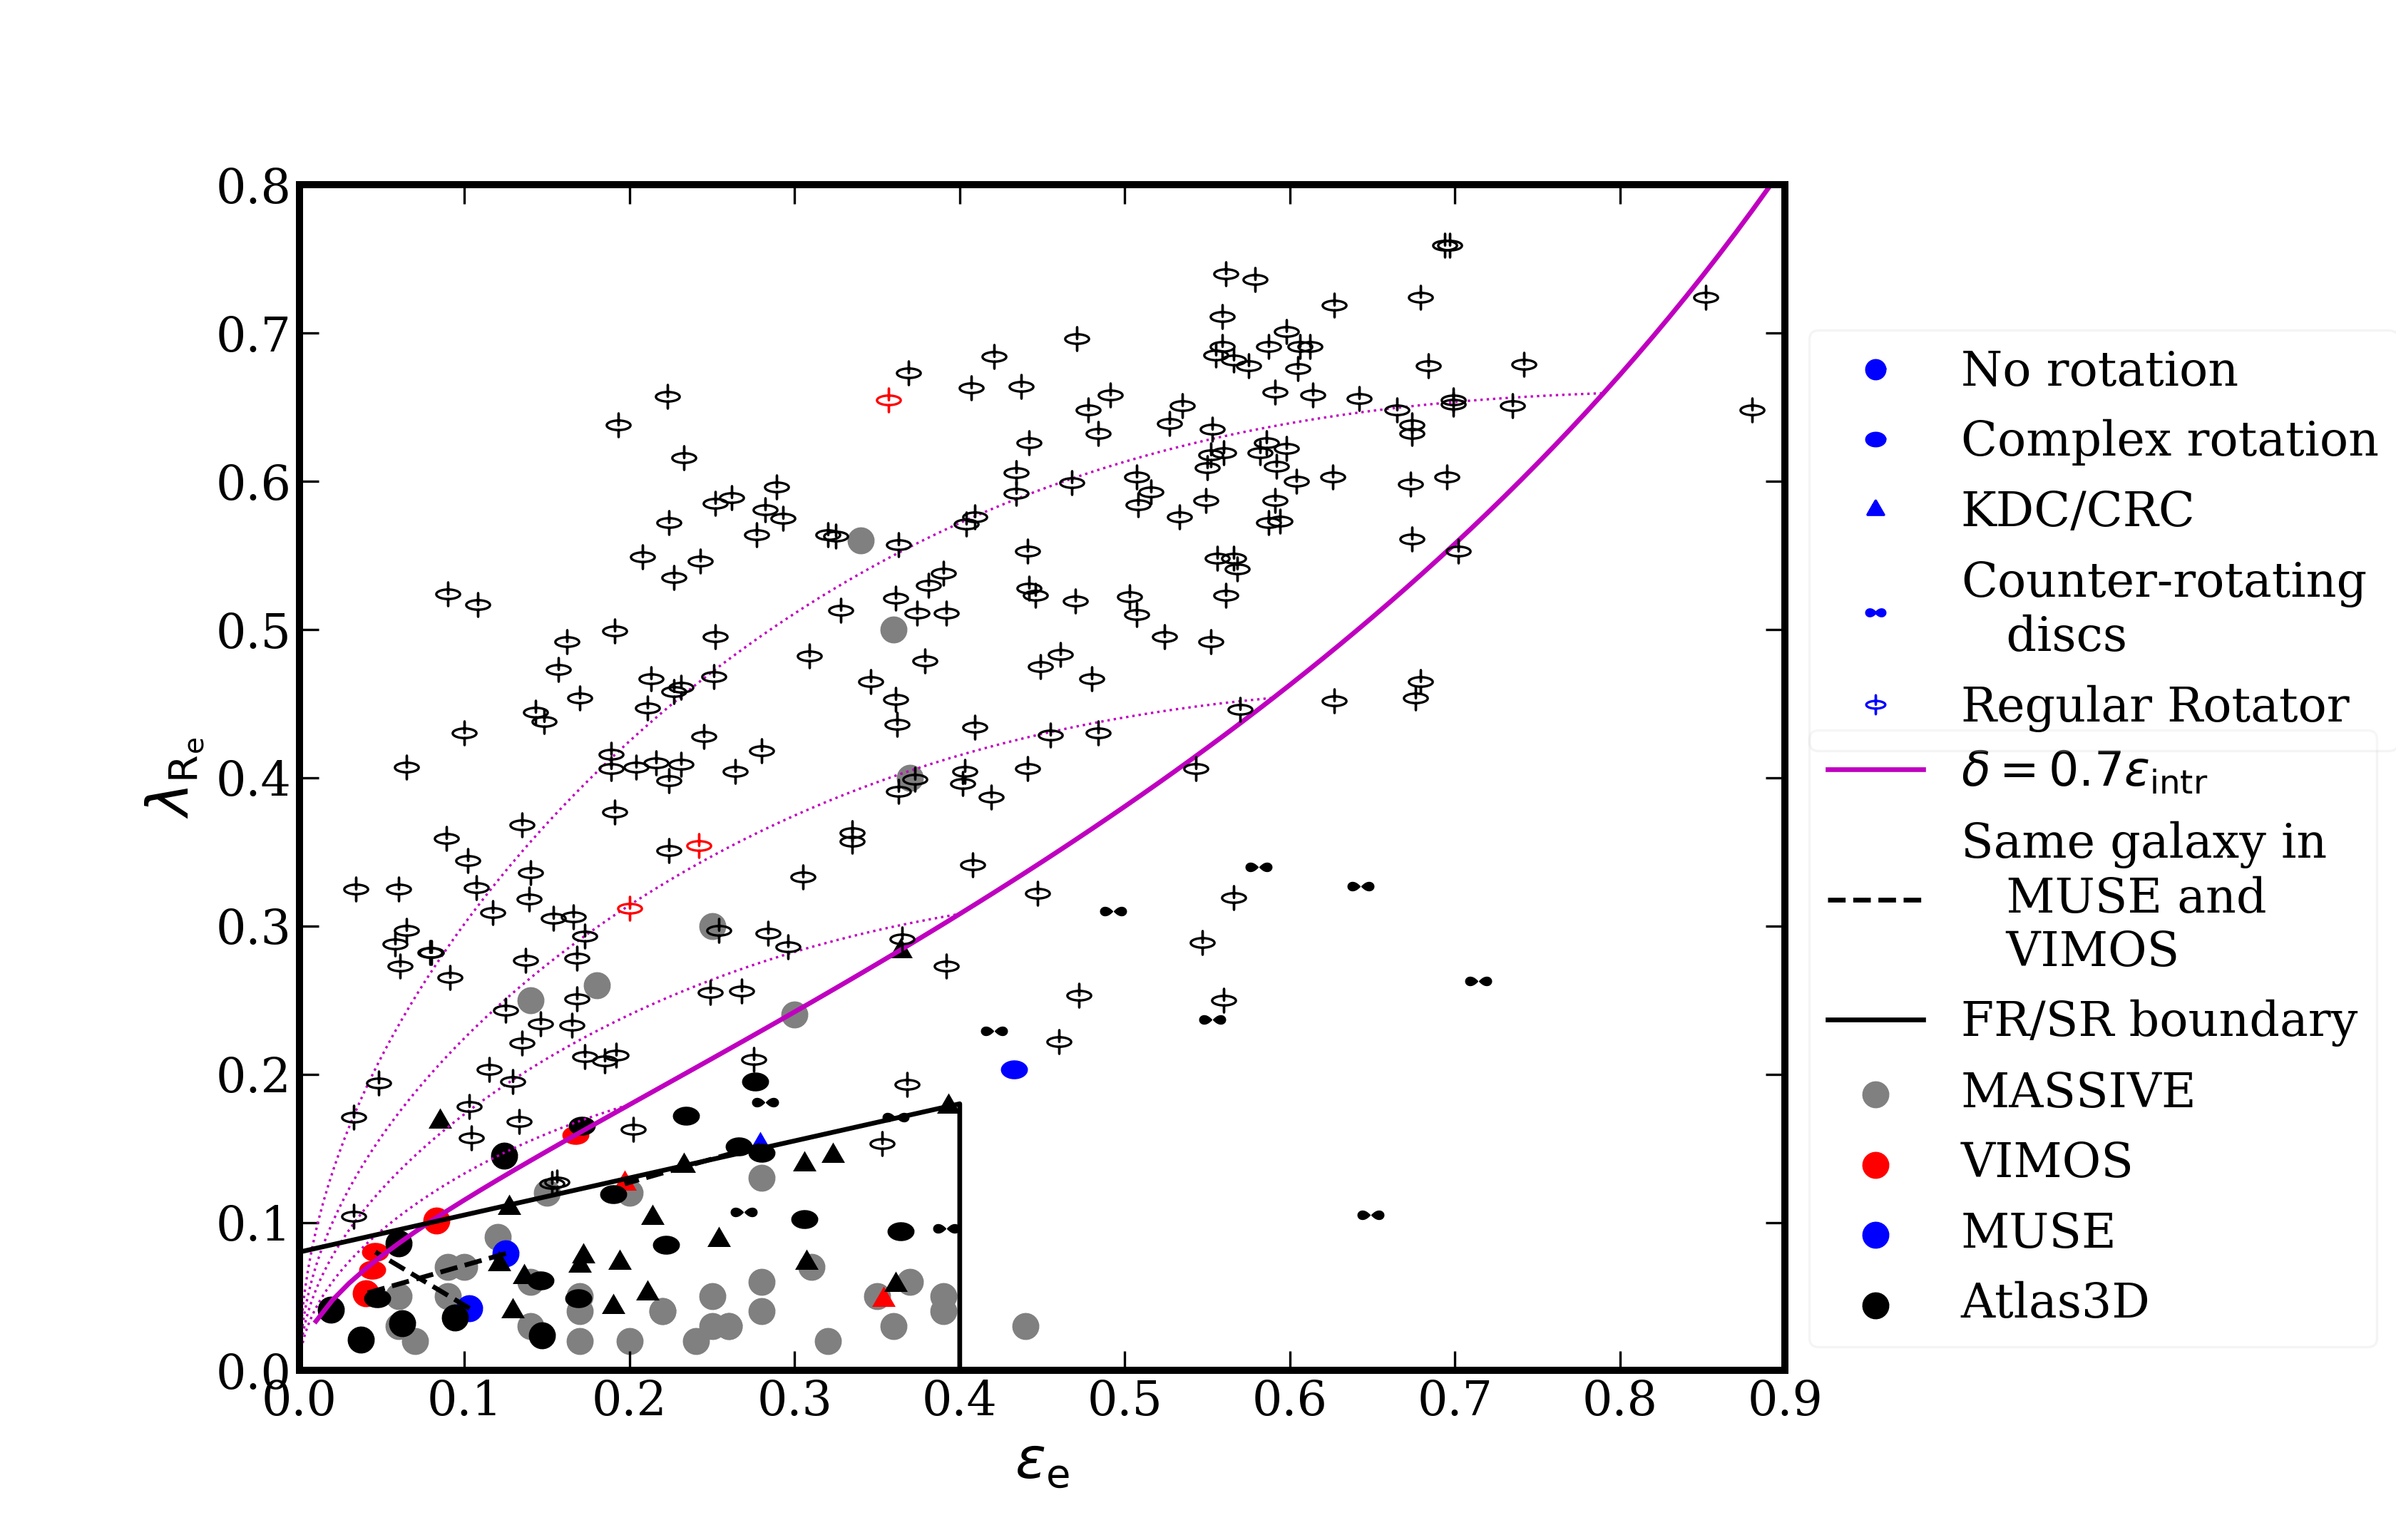
\includegraphics[width=0.85\textwidth]{chapter4/lambda_R_ellipticity.png}
				\caption[$\lambda_\mathrm{R_e}$ -- ellipticity diagram]{$\lambda_\mathrm{R_e}$ -- ellipticity diagram. VIMOS and MUSE measurements are shown in red and blue, respectively. For comparison, Atlas$^\text{3D}$ galaxies \citep{Emsellem2011} are shown in black and MASSIVE galaxies \citep{Veale2017} in grey. The theoretical limit (edge-on systems) of disc-dominated galaxies is shown in solid magenta, with lines of constant intrinsic angular momentum but varying inclination in dotted magenta. The black solid lines show the limits of the fast-/slow-rotator classes. The MASSIVE survey does not report substructure, so the MASSIVE sample galaxies are shown with filled circles.}
				\label{fig:lambdaR_ellip}
			\end{figure}
			We find that 5 out of 11 galaxies, or $(45\pm13)$\%, are slow rotators. This very different to that of the Atlas$^\text{3D}$ and MASSIVE samples, which find 13.1\% and 77.5\%, respectively. However, slow rotators are more likely to be found in higher mass galaxies and the three samples (Atlas$^\text{3D}$, MASSIVE and our Southern sample) have very different mass distributions (see upper panel of Fig.\,\ref{fig:SRmassFraction}).

			In order to account for the difference in mass distribution, we find the expected fraction of slow rotators in the Southern sample, $f'$, corrected to the mass distribution of the combined Atlas$^\text{3D}$ and MASSIVE samples (hereafter the A+M sample), as
			\begin{equation}
				f' = \sum_{i=0}^N N^\mathrm{SS}_i f^\mathrm{CS}_i \, , 
			\end{equation}
			where $N^\mathrm{SS}_i$ is the number of Southern sample galaxies in the $i^\mathrm{th}$ mass bin, $N^\mathrm{CS}_i$ is the fraction of slow rotators in the $i^\mathrm{th}$ mass bin in the A+M combined sample and $N$ is the total number of mass bins. In our case we use the $K$-band absolute magnitude ($M_K$) as a proxy for stellar mass, with bins of 0.5 mag. This gives $f' = 0.64 \pm 0.06$, consistent with our finding of $(45\pm13)$\% of the Southern sample galaxies being slow rotators, particularly considering the low number statistics of the Southern sample. There is, therefore, no discernible difference in the fraction of galaxies that are slow-rotators between our radio-selected Southern sample and the optically-selected A+M sample, once differences in the mass distributions are taken into account. 

			\begin{figure}
				\centering
				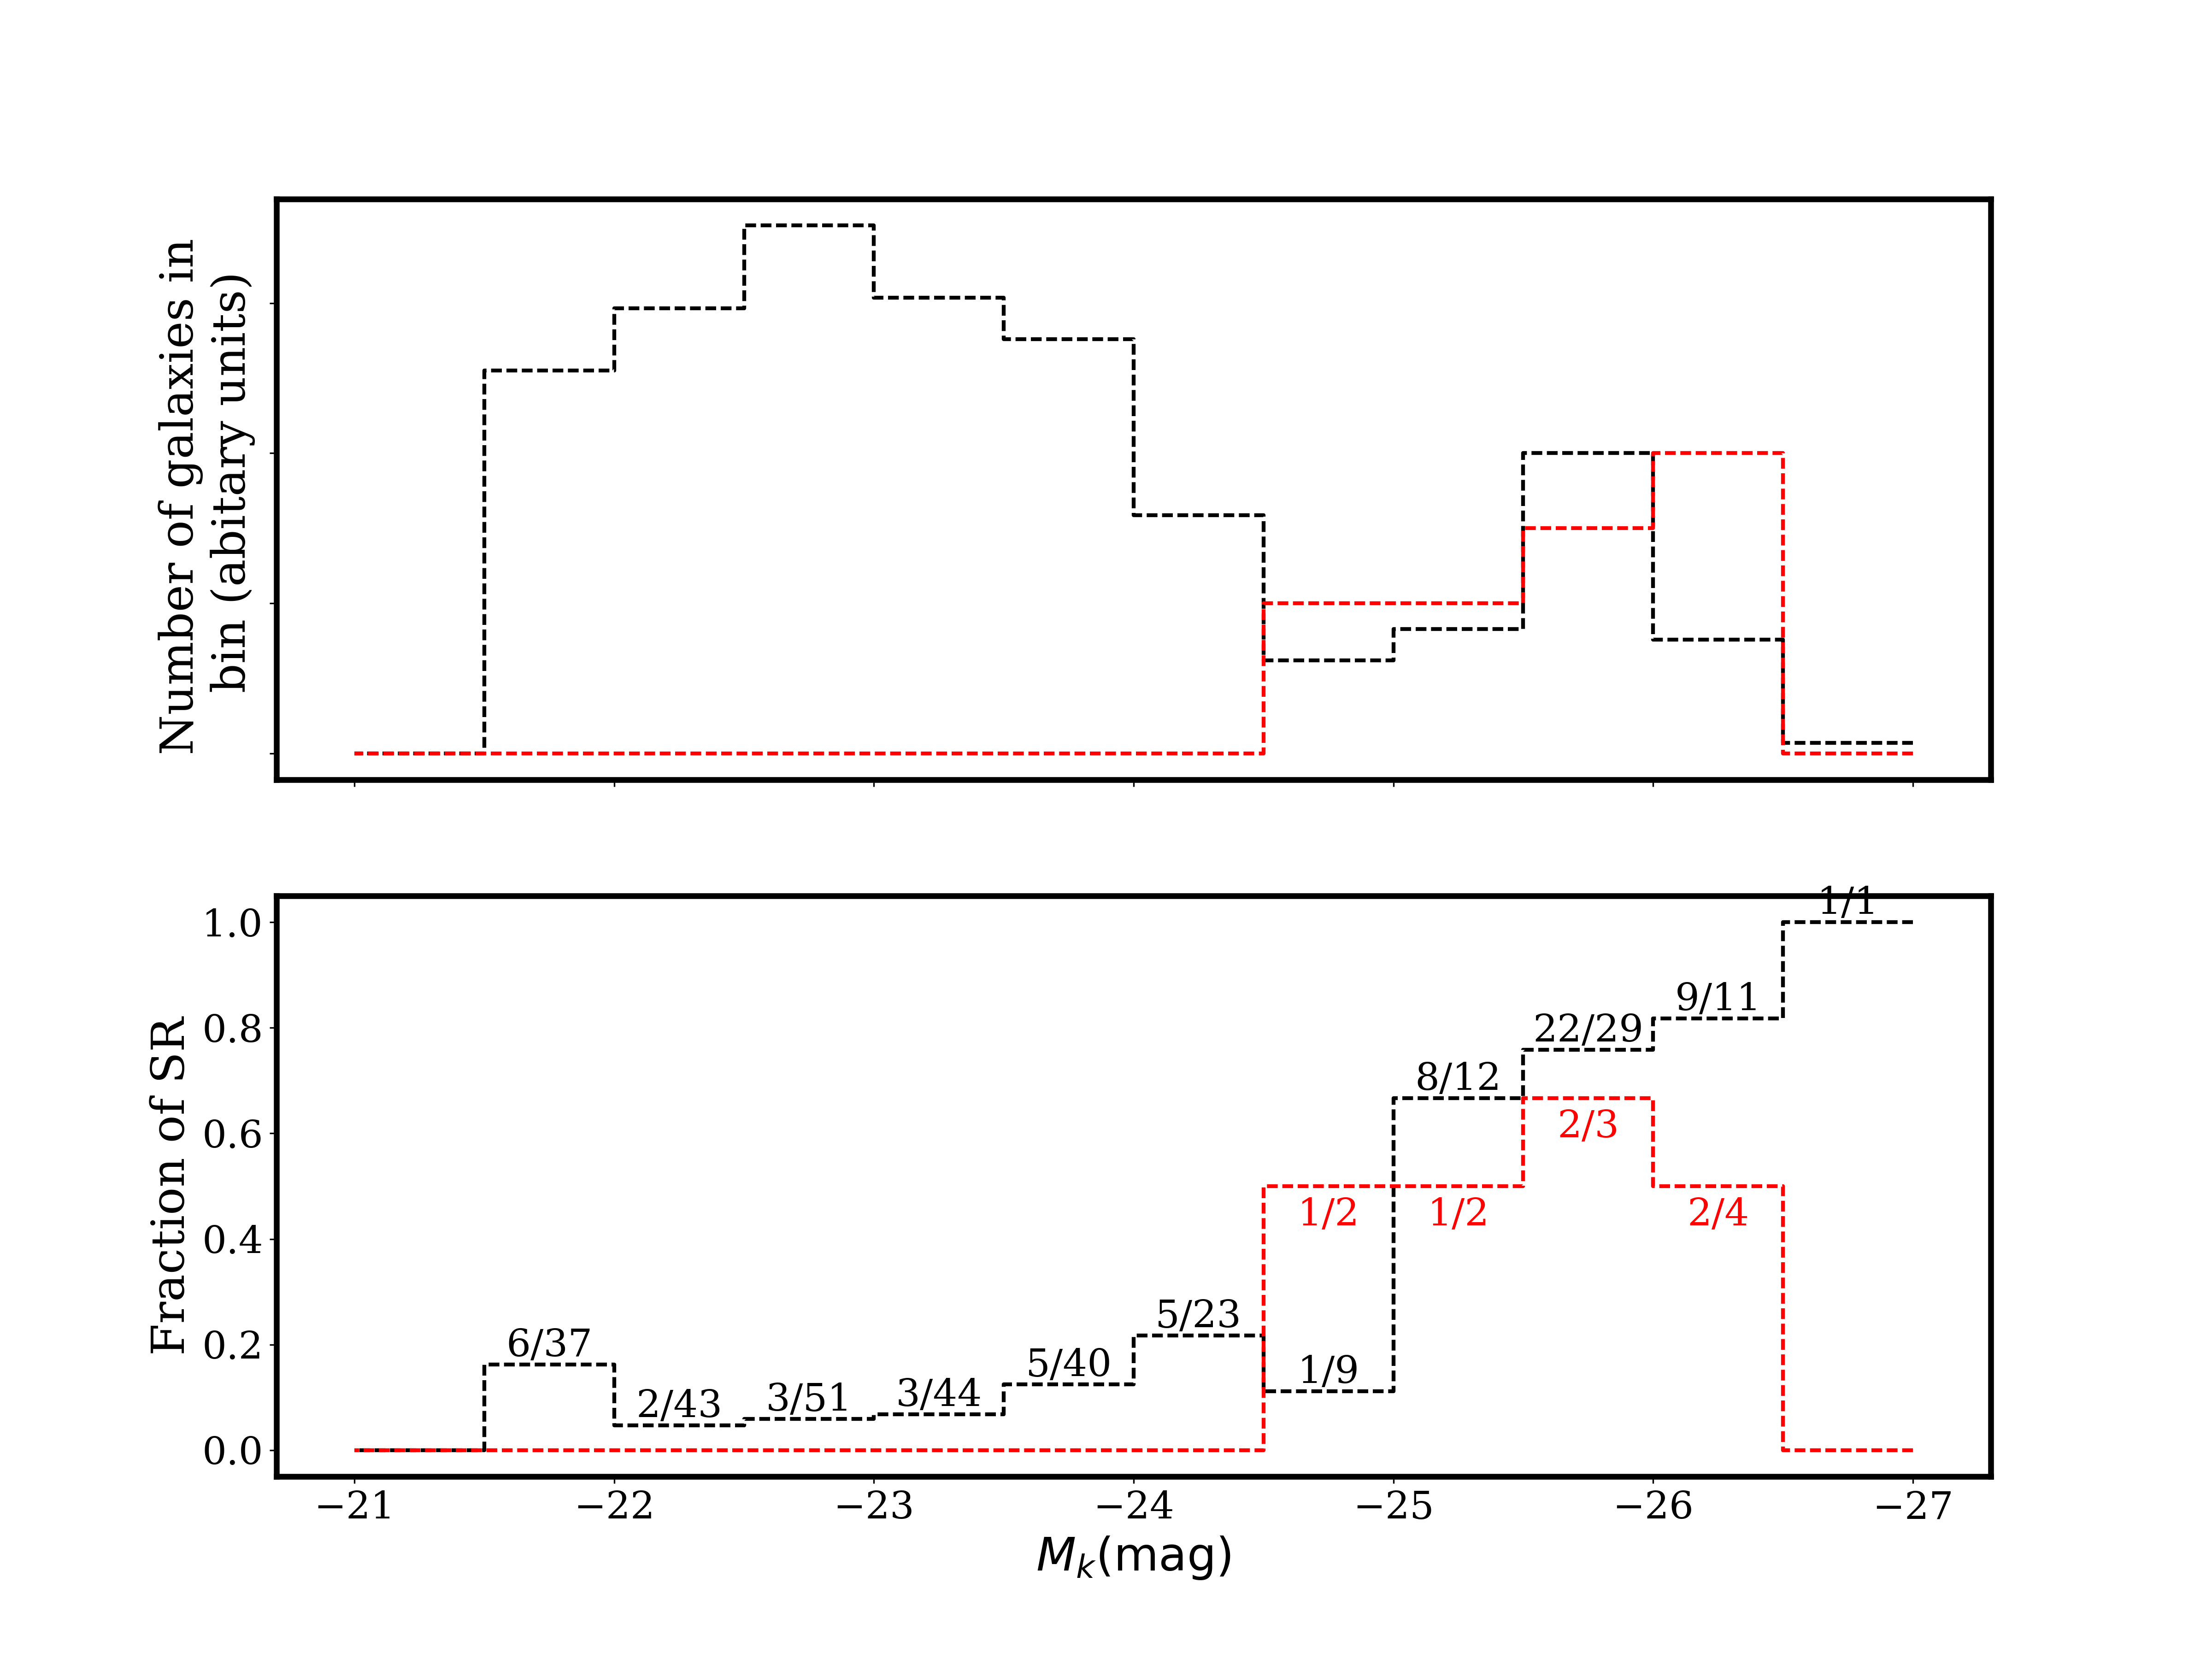
\includegraphics[width=0.8\textwidth]{chapter4/M_k_binned.png}
				\caption[Mass matching global kinematics]{Upper panel: mass distribution of the A+M sample (black) and of our Southern sample (red). Lower panel: fraction of slow rotators within each mass bin. The labels list the number of slow rotators and total number of galaxies in each bin.}
				\label{fig:SRmassFraction}
			\end{figure}

		\subsection{Radial Angular Momentum Profile}
			\label{subsec:ResolvedLambda_R}
			The radial $\lambda_R$ profiles (i.e. $\lambda_R$ as a function of aperture radius) are shown in Fig.\,\ref{fig:lambdaR_profile}. We see, with the exception of IC 1531, a disc with very low inclination, fast and slow rotators are separated by $\approx 0.3\,\mathrm{R_\odot}$. We also see that most of the fast rotators of our Southern sample have a rapidly rising $\lambda_R$ profile, which flatten out by $\approx 0.5\,\mathrm{R_\odot}$. This is consistent with the SAURON surveys findings \citep[e.g.][Fig.\,2]{Emsellem2007}. 

			\begin{figure}
				\centering
				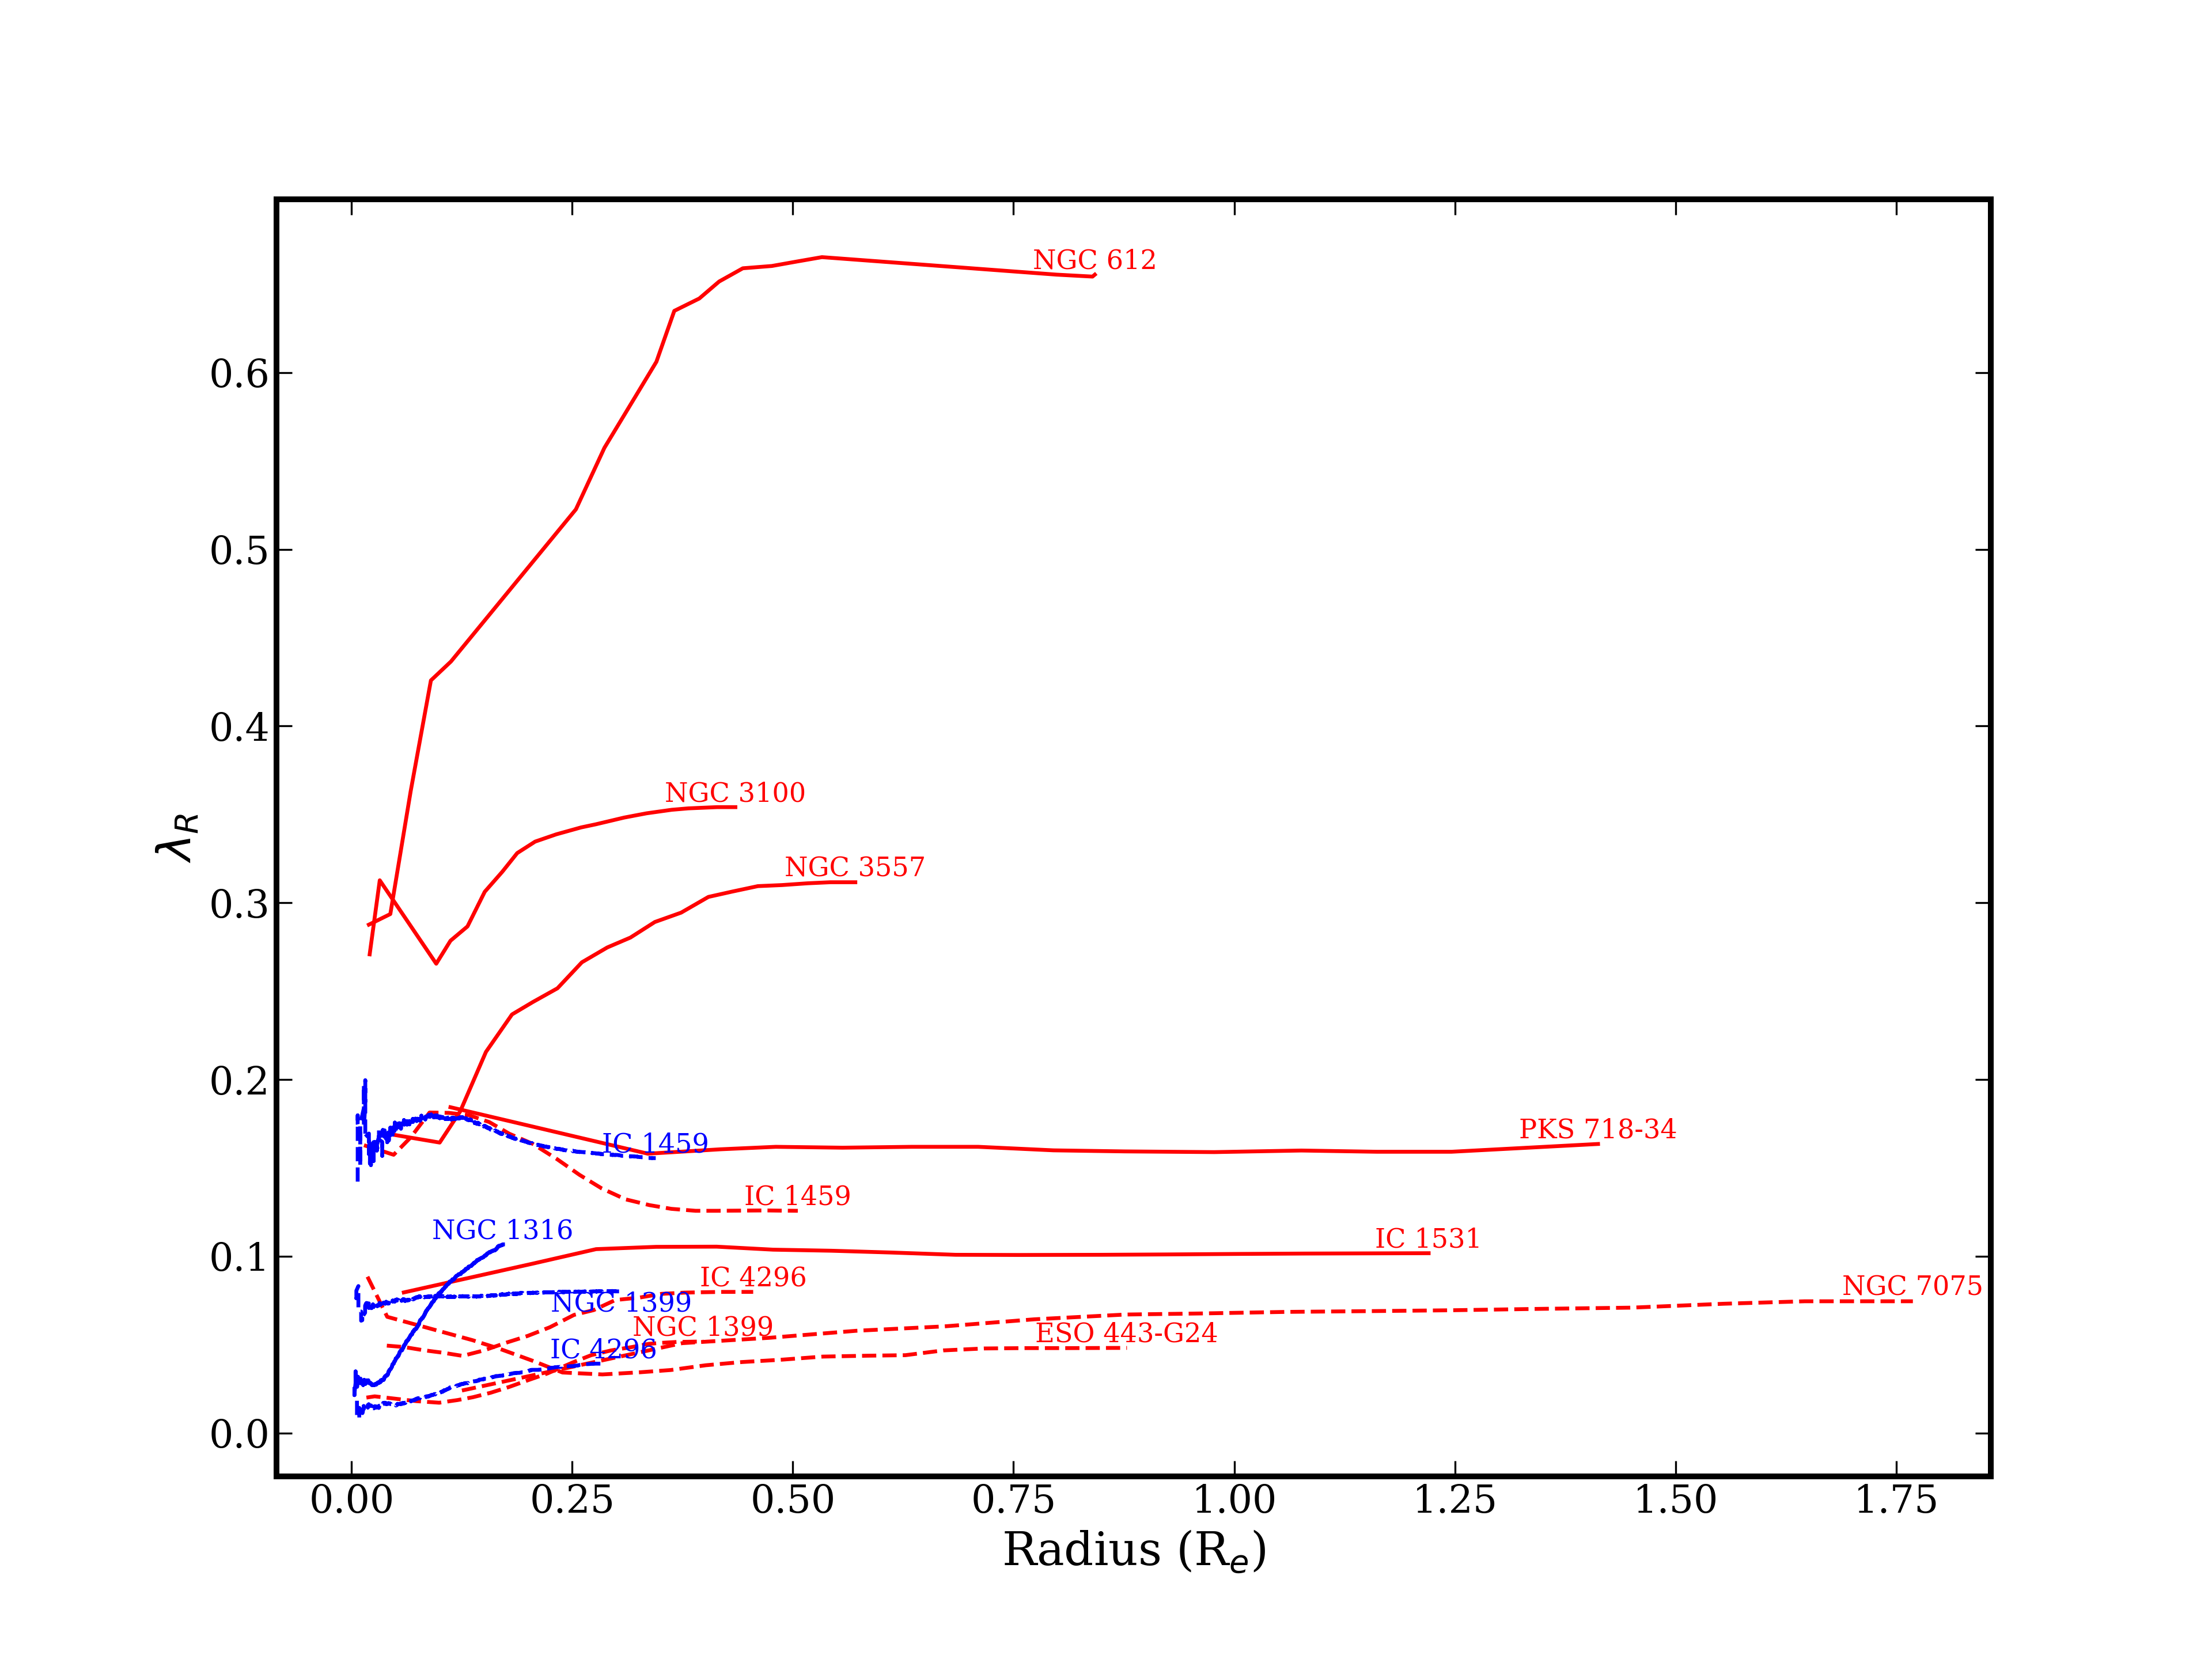
\includegraphics[width=.7\textwidth]{chapter4/lambda_R.png}
				\caption[$\lambda_{R}$ radial profiles]{Radial $\lambda_{R}$ profiles. Profiles derived from VIMOS data are in blue, while those derived from MUSE data are in red. Solid lines represent fast rotators; dashed lines, slow rotators.}
				\label{fig:lambdaR_profile}
			\end{figure}

		
% Change to intrinsic shape? - discuss ellipticity
		\subsection{Intrinsic Shape}
			\label{subsec:Misalignment}

			The photometric position angle, $PA_\text{phot}$, is defined as the angle westwards from North of semi-major axis of the largest best-fitting ellipse as found in Section \ref{fig:Ellipticity}.  

			The kinematic position angle, $PA_\text{kin}$, is defined as the angle of the axis perpendicular to the apparent angular momentum vector westwards from North. A global value of $PA_\text{kin}$ is found using the \textsc{python} routine \textsc{fit\_kinematic\_pa}\footnote{http://www-astro.physics.ox.ac.uk/\~mxc/software/\#pa\_kin} as described in appendix C of \citet{krajnovic2006}. This routine finds a symmetric (about $PA_\text{kin}$) velocity field, by replacing the mean velocity, $V$, in each bin with
			\begin{equation}
				V'(x, y) = \frac{V(x,y) + V(x, -y) - V(-x,y) - V(-x,-y))}{4} \,,
			\end{equation}
			where $x$ and $y$ are the centroid coordinates of a given bin, with the origin at the centre of the galaxy and the x axis aligned along $PA_\text{kin}$. Linear interpolation is used where necessary.

			Column 4 in Table \ref{tab:classify} lists the misalignments between the photometric and kinematic position angles, $\Gamma_\text{kin} \equiv \arcsin\sin\left( PA_\text{phot} - PA_\text{kin} \right)$. As described in Section \ref{sec:ETG}, while is cannot be used to describe the intrinsic shape of an individual galaxy, it can be used in a statistical way. We find all the regular rotators in our Southern sample, are consistent with having aligned photometry and kinematic position angles to within 11\degree, while non-regular rotators have a large range of values of $\Gamma_\text{kin}$. IC 1531, NGC7075 and PKS 718-34 all have very large uncertainties in the value of $PA_\text{phot}$ due to the VIMOS quadrant artifacts causing the fitting routine of \textsc{kinemetry} to become unreliable. 


			






			\citet{Cappellari2007}, \citet{Krajnovic2011} and \citet{Fogarty2015} all showed that regular rotators almost always have aligned photometric and kinematic axes (with a scatter of 4$\degree$). 

% CHeck numbers here - issue with uncertainty from KINEMETRY
			Regular rotators with a significant misalignment are either very round, interacting or strongly barred (see Fig.\,\ref{fig:Misalignment}). Taking into account the lower quality of our data, our results are consistent with this. Of the 4 regular rotators in our Southern sample, 2 are misaligned by less than 8$\degree$ (NGC 612 and NGC 3557) and the other 2 are round ($\epsilon < 0.3$; IC 4296 and NGC 3100). As noted in \citet{Cappellari2016}, this result requires that regular rotators are axisymmetric.

			Misalignments between the photometric and kinematic position angles are routinely observed for non-regular rotators. This generally implies a more triaxial intrinsic shape, although large misalignments are extremely rarely observed in galaxies with $\epsilon > 0.4$, suggesting that non-regular rotators are more spherical in shape. This is the reason for the $\epsilon < 0.4$ requirement in the definition of slow rotators. The non-regular rotators in our sample indeed all have $\epsilon < 0.4$.


\section{Stellar Population}
	\label{sec:pop}
	As described in Section \ref{subsec:PopFit}, in order to find the best-fitting stellar populations for our Southern sample, we must first measure the absorption line strengths of the indices in Table \ref{tab:tab:abIndex}. We first present maps of the strength of each index (Section \ref{subsec:absorption}), before examining the Mg -- $\sigma$ relation (Section \ref{subsubssec:Mgsigma}), comparing the measured line strengths to the literature (Section \ref{{subsubsec:Lit}}) and finally presenting maps of the stellar populations (Section \ref{subsec:ssp}).

	\subsection{Absorption Line Strengths}
		\label{subsec:absorption}

		Figs.\,\ref{fig:VIMOS_absorption} and \ref{fig:MUSE_absorption} show the spatially-resolved absorption line strengths of our Southern sample galaxies. For the VIMOS datacubes, we measure the G4300, Fe4383, Ca4455, Fe4531, H\,$\beta$, Fe5015 and Mg\,b indices, as defined in Table \ref{tab:abIndex}. For the most distant galaxies (NGC 612 and PKS 718-34), the red continuum band of the Mg\,b is redshifted beyond the spectral range of the VIMOS spectrograph. In these cases we have not attempted to adjust the definition of the Mg\,b index bandpass (as \citealt{Kuntschner2006} did with defining Fe5270s to use instead of Fe5270), but have simply not included Mg\,b in any future analysis of these galaxies. For the MUSE datacubes, we measure the H\,$\beta$, Fe5015, Mg\,b, Fe5270, Fe5335, Fe5406, Fe5709, Fe5782, NaD, TiO1 and TiO2 indices, also defined in Table \ref{tab:abIndex}.

		\begin{figure}
			\centering
			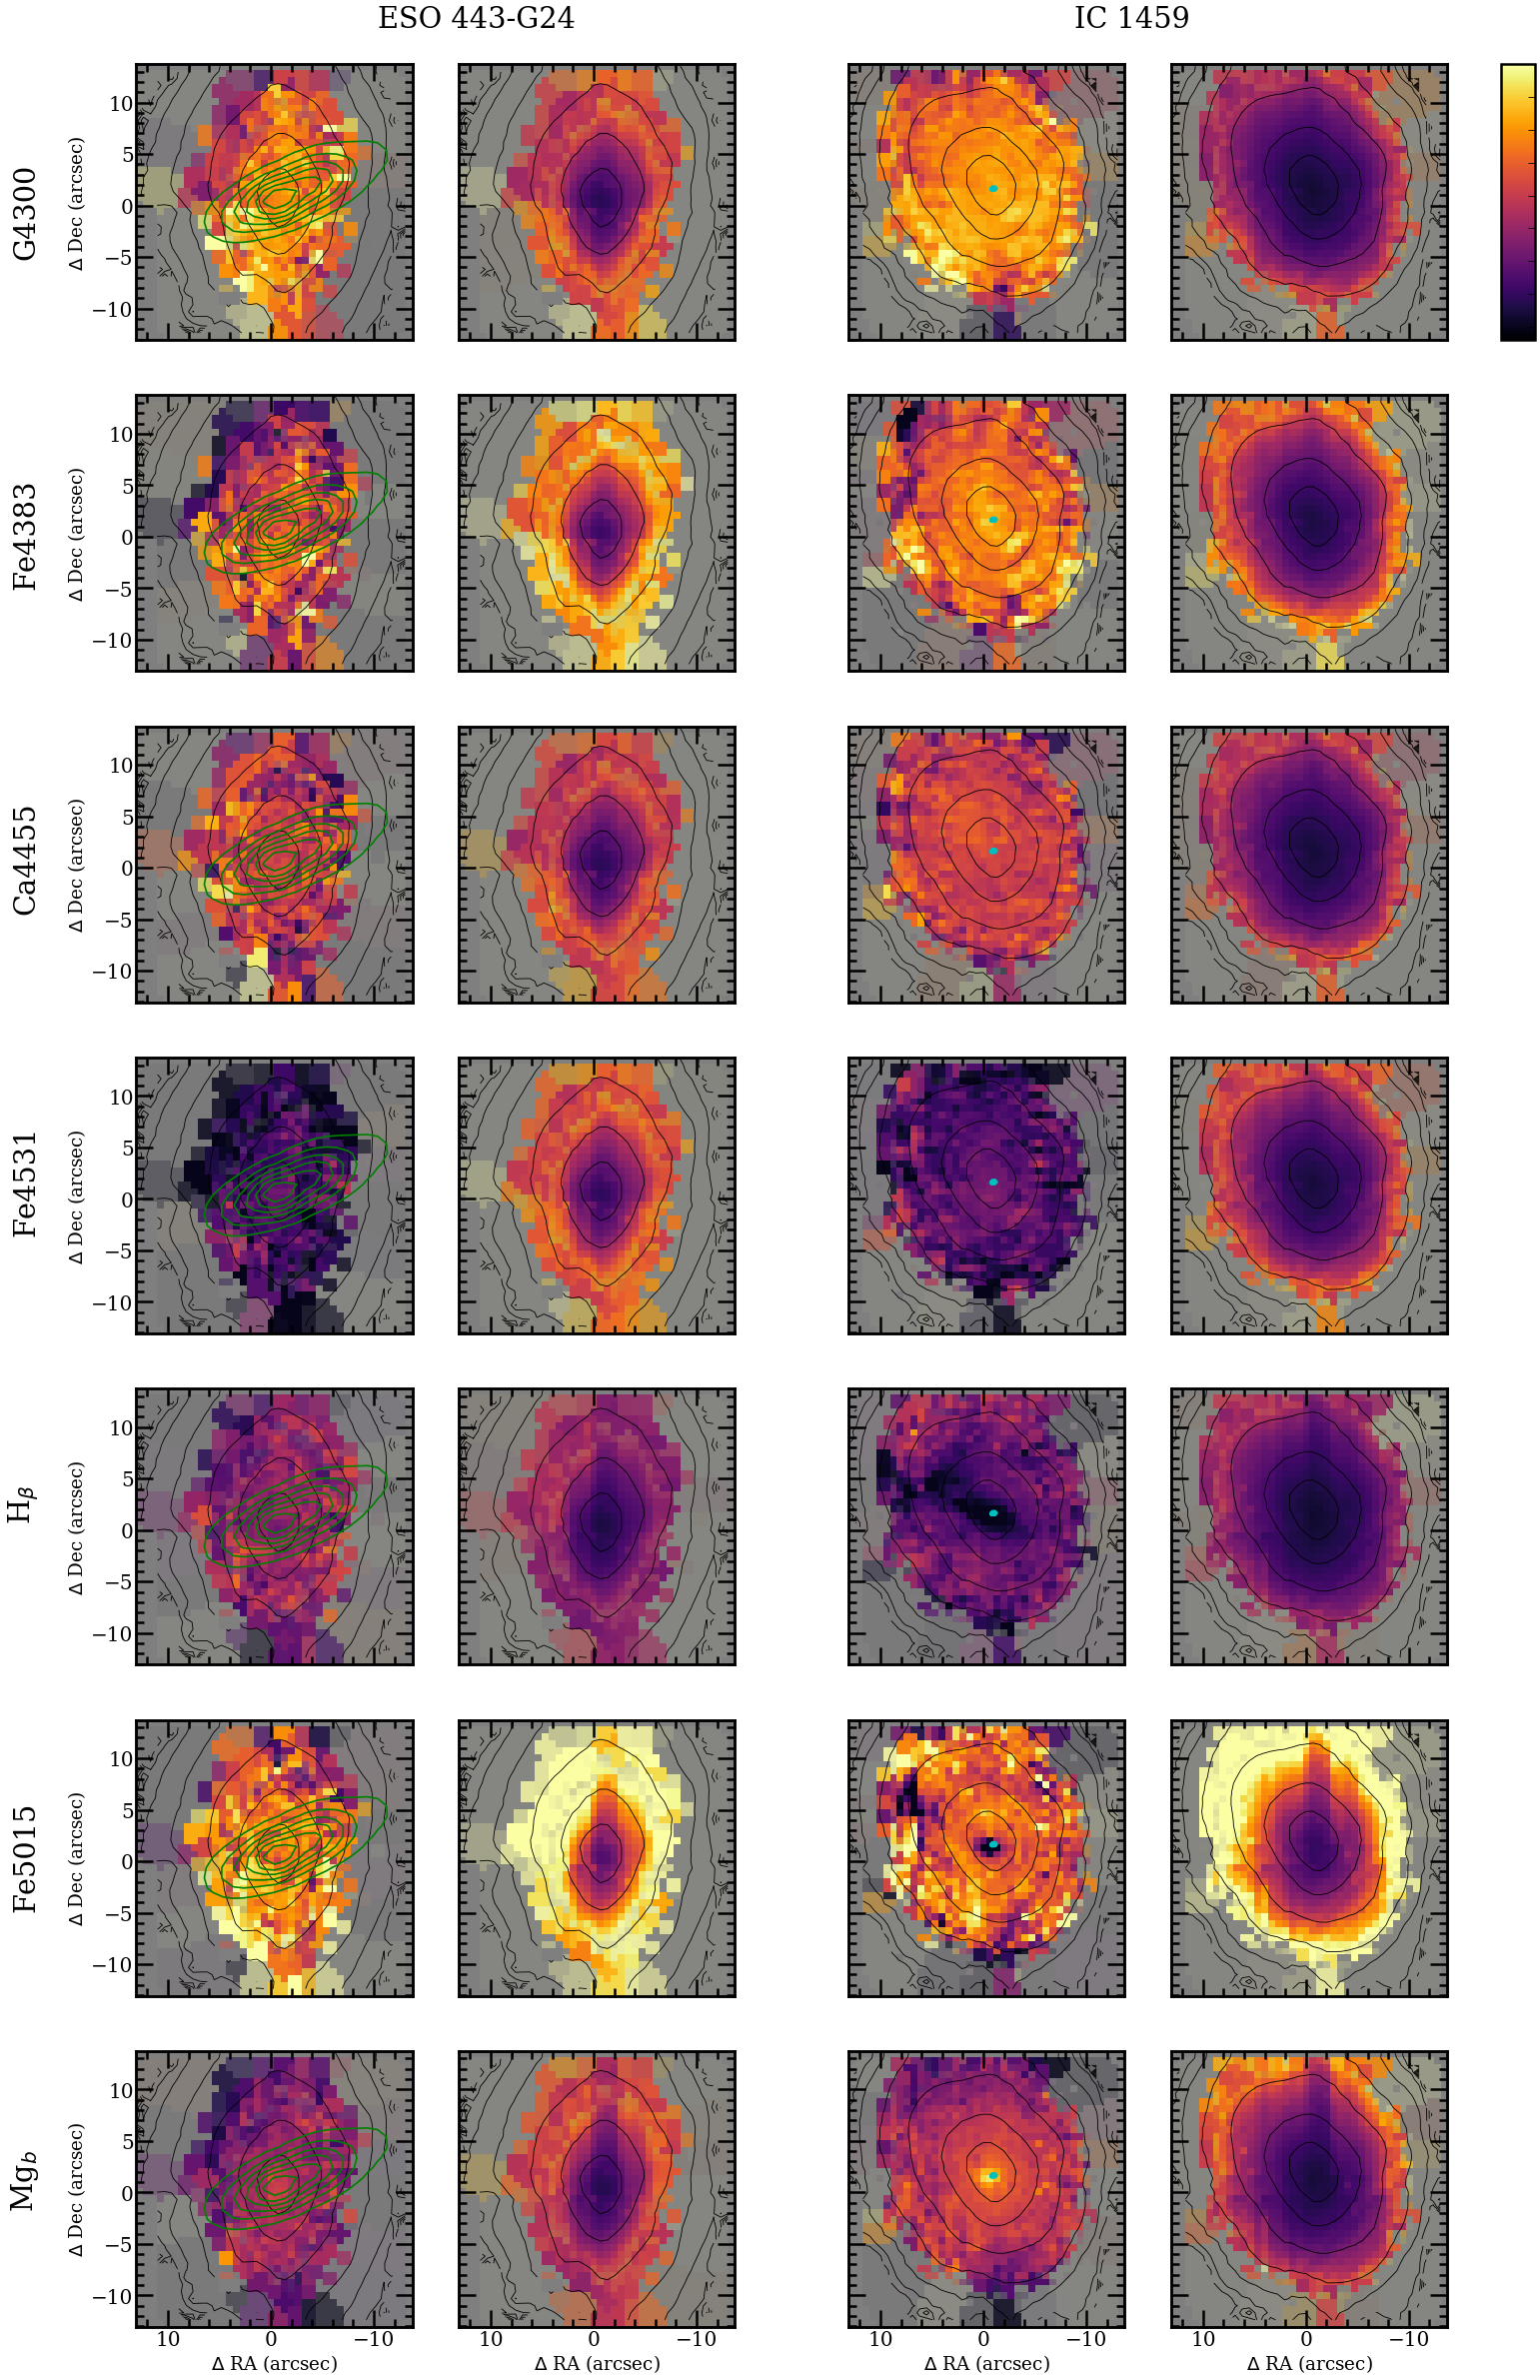
\includegraphics[height=0.94\textheight]{chapter4/vimos/abs1.png}
			\caption[VIMOS absorption line strength maps]{VIMOS absorption line strength maps. Left to right: ESO 443-G24 line index and associated uncertainties, IC 1459 line index and associated uncertainties. Top to bottom: G4300, Fe4383, Ca4455, Fe4531, H\,$\beta$, Fe5015 and Mg\,b index. Contours are as in Fig.\,\ref{fig:VIMOS_stellar}. Limits on the colour scales are 0.5--3.5\,\AA\ for H\,$\beta$ and Ca4455 line strengths, 3--7\,\AA\ for all other line strengths and 0--0.5\,\AA\ for the associated uncertainties.}
			\label{fig:VIMOS_absorption}
		\end{figure}
		\begin{figure}
			\centering
			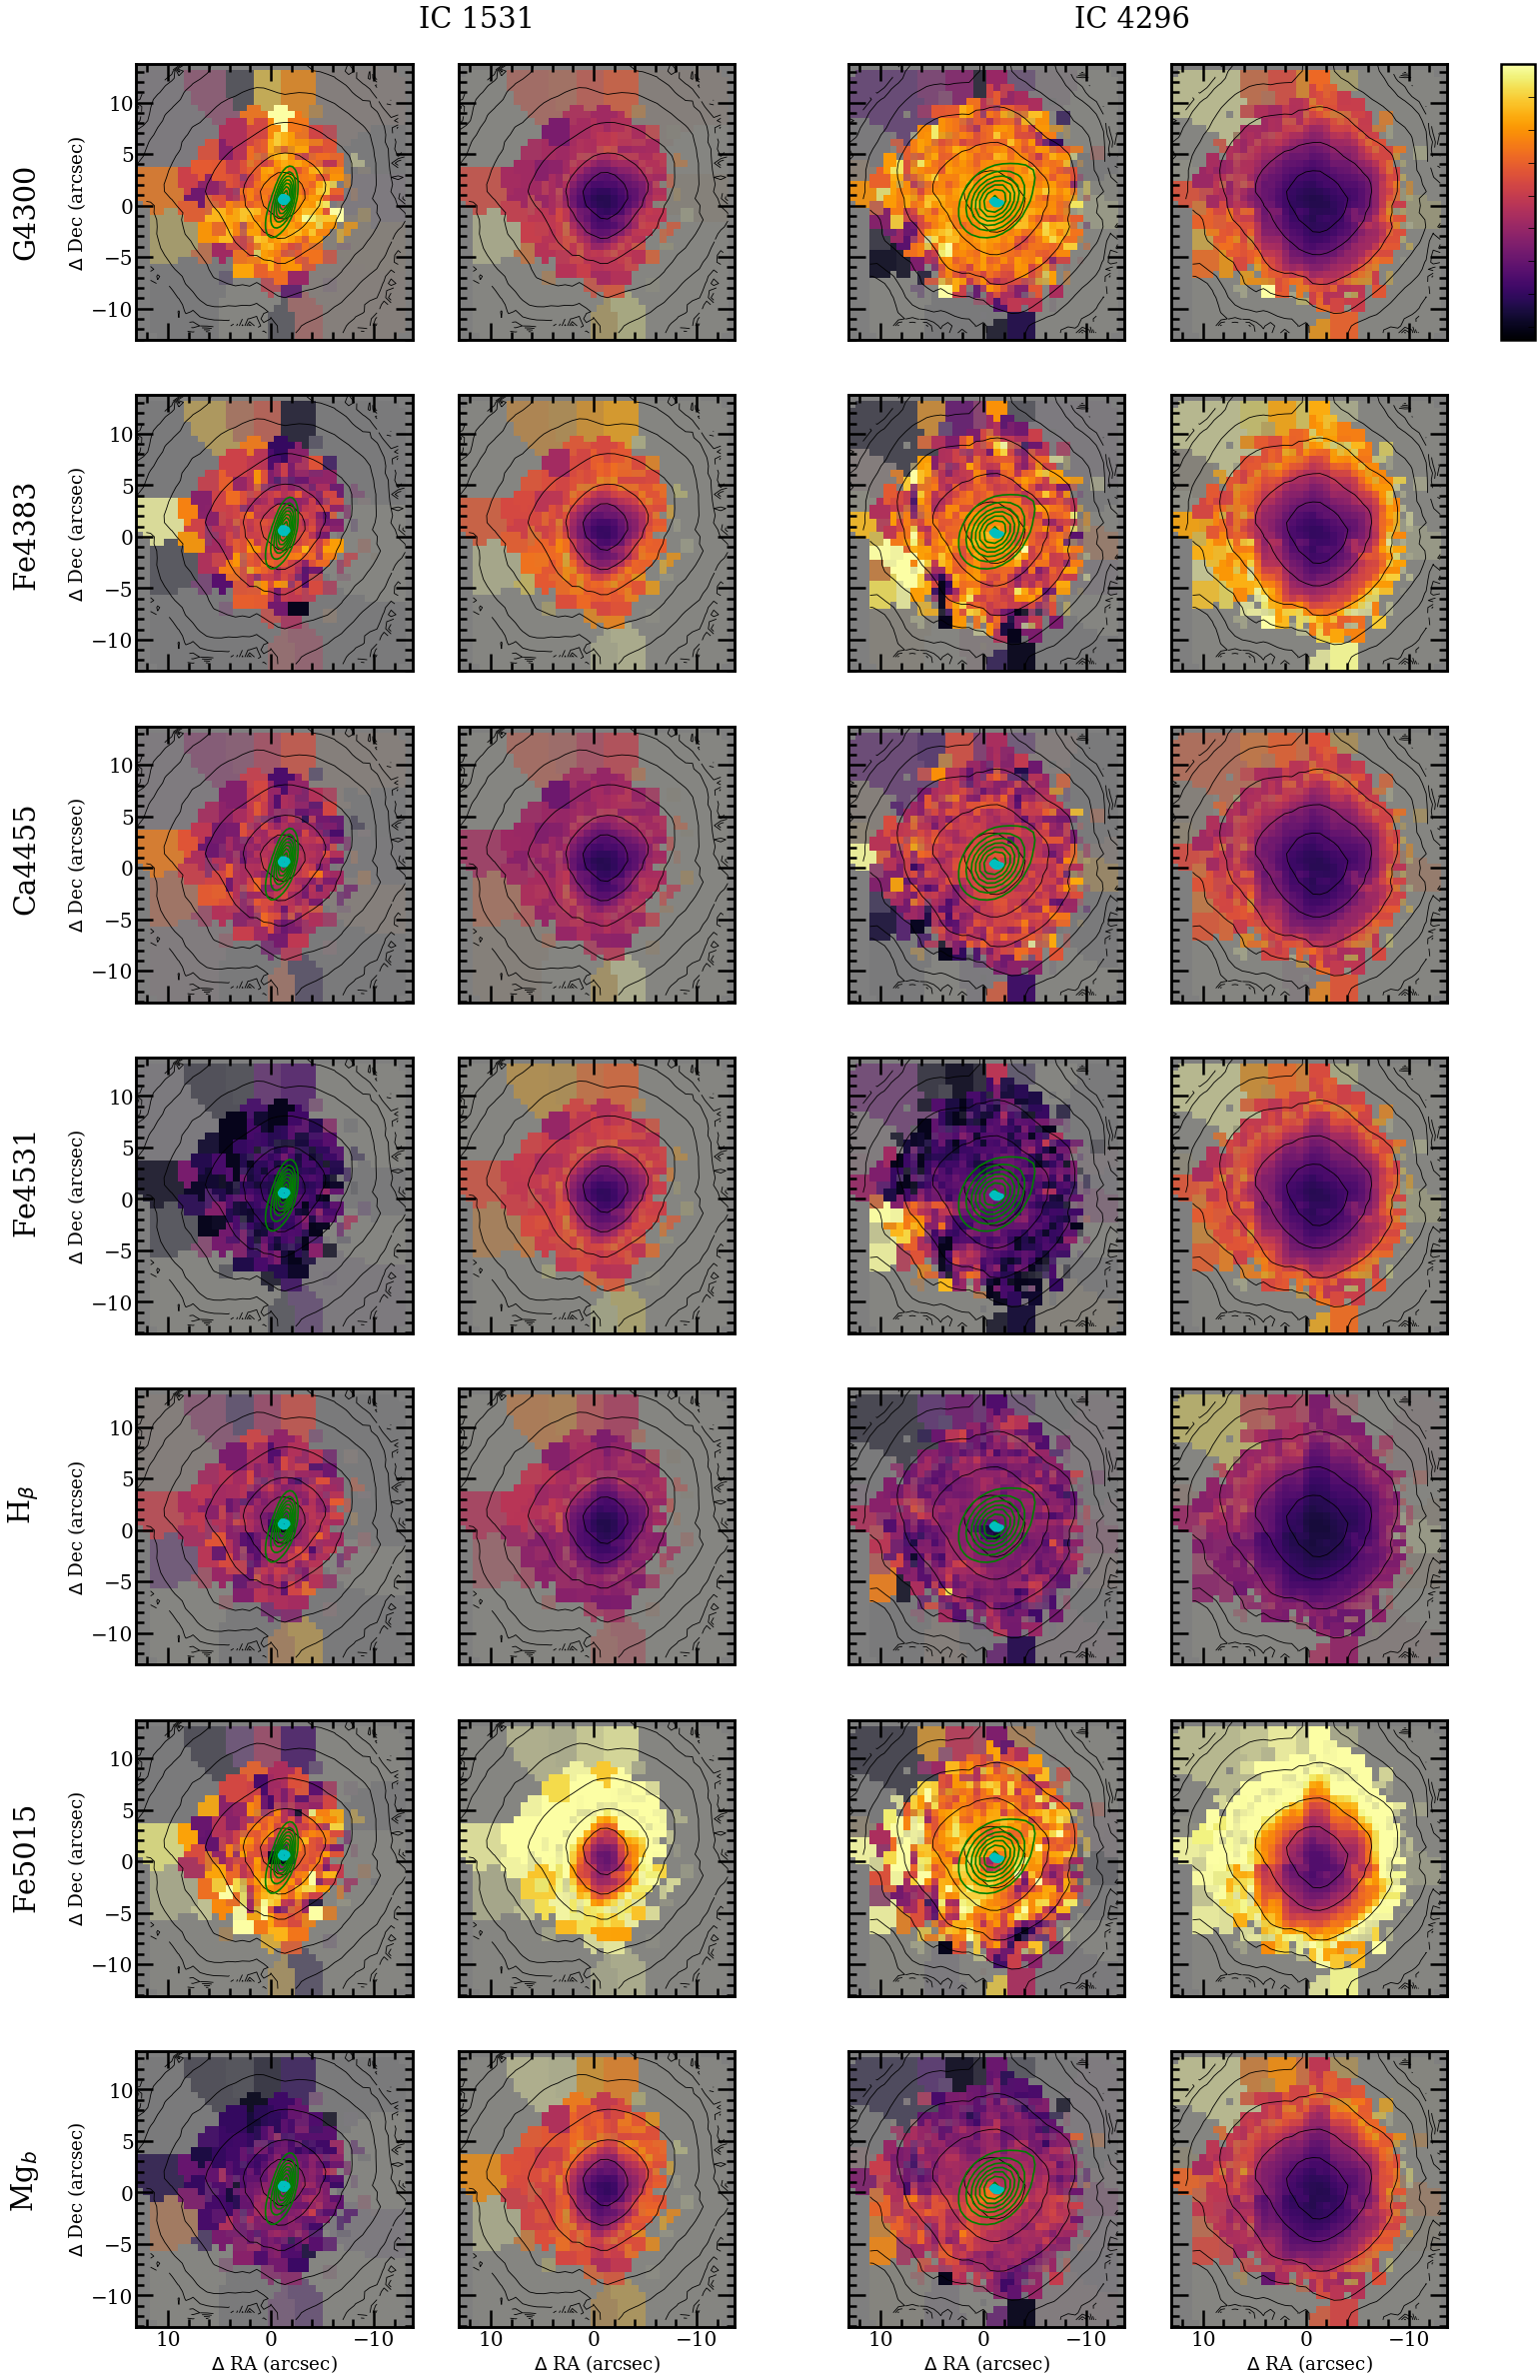
\includegraphics[height=0.94\textheight]{chapter4/vimos/abs2.png}
			\contcaption{\textit{Continued.}}% for IC 1531 and IC 4296.}
		\end{figure}
		\begin{figure}
			\centering
			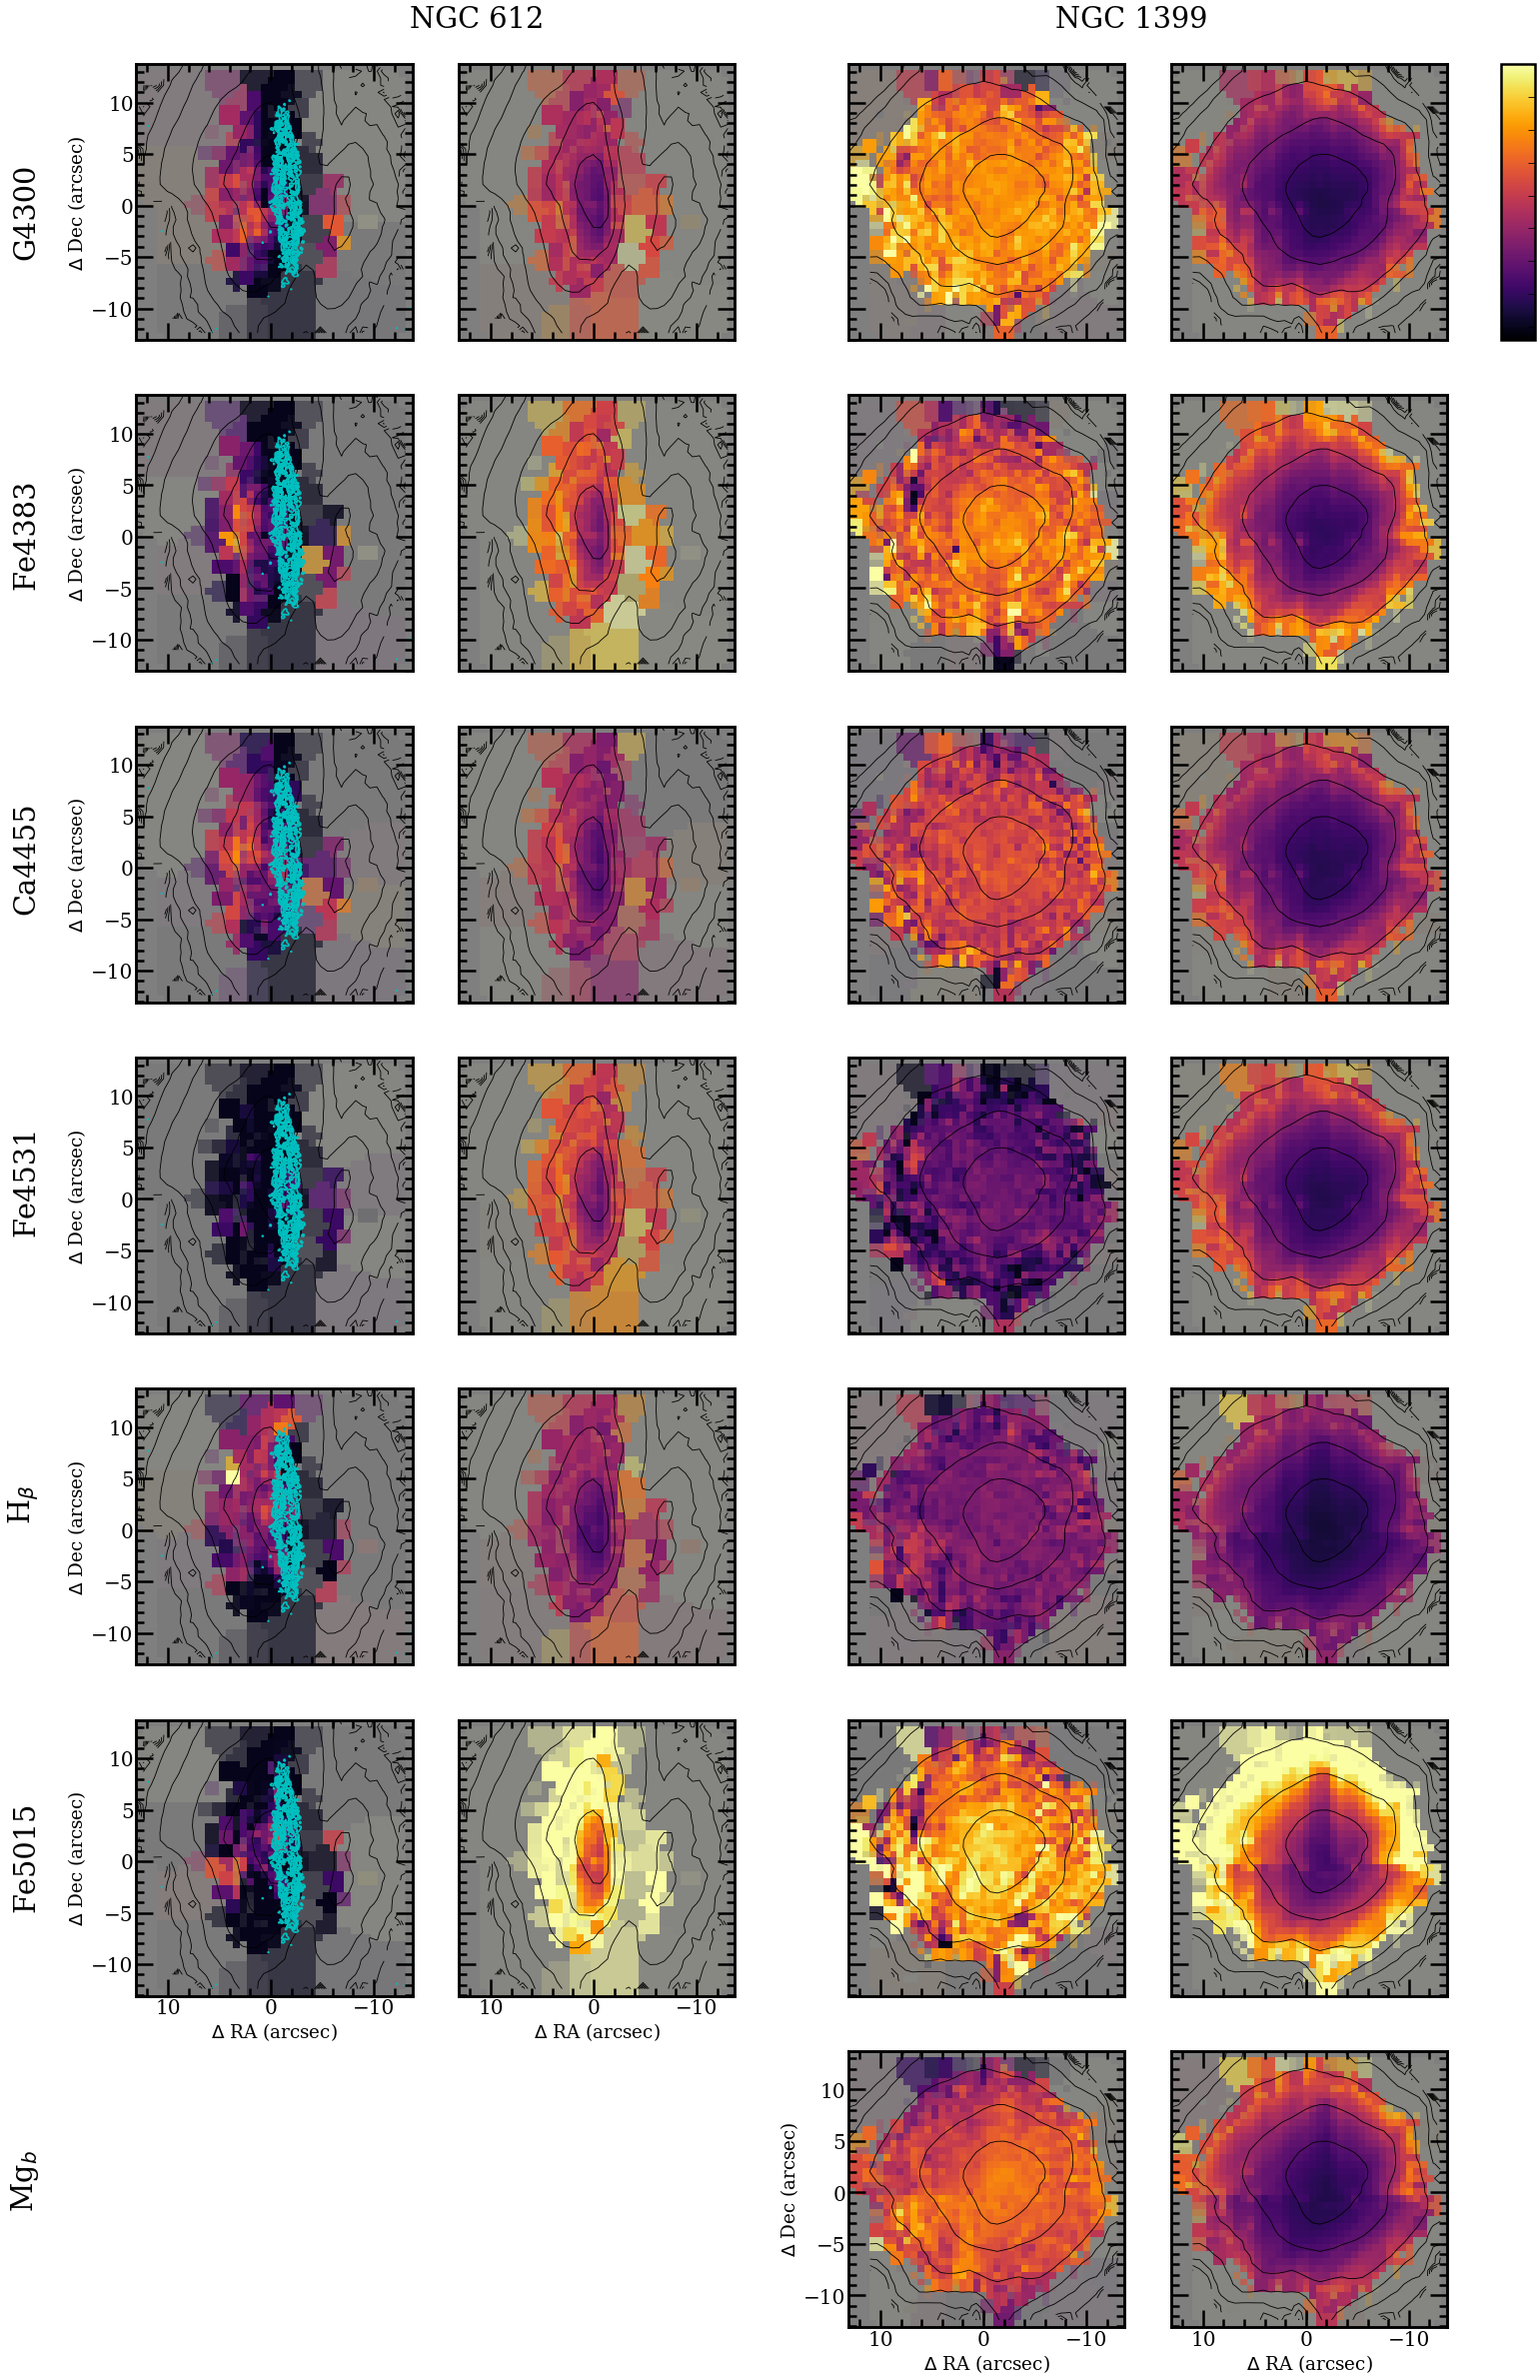
\includegraphics[height=0.94\textheight]{chapter4/vimos/abs3.png}
			\contcaption{\textit{Continued.}}% for NGC 612 and NGC 1399}
		\end{figure}
		\begin{figure}
			\centering
			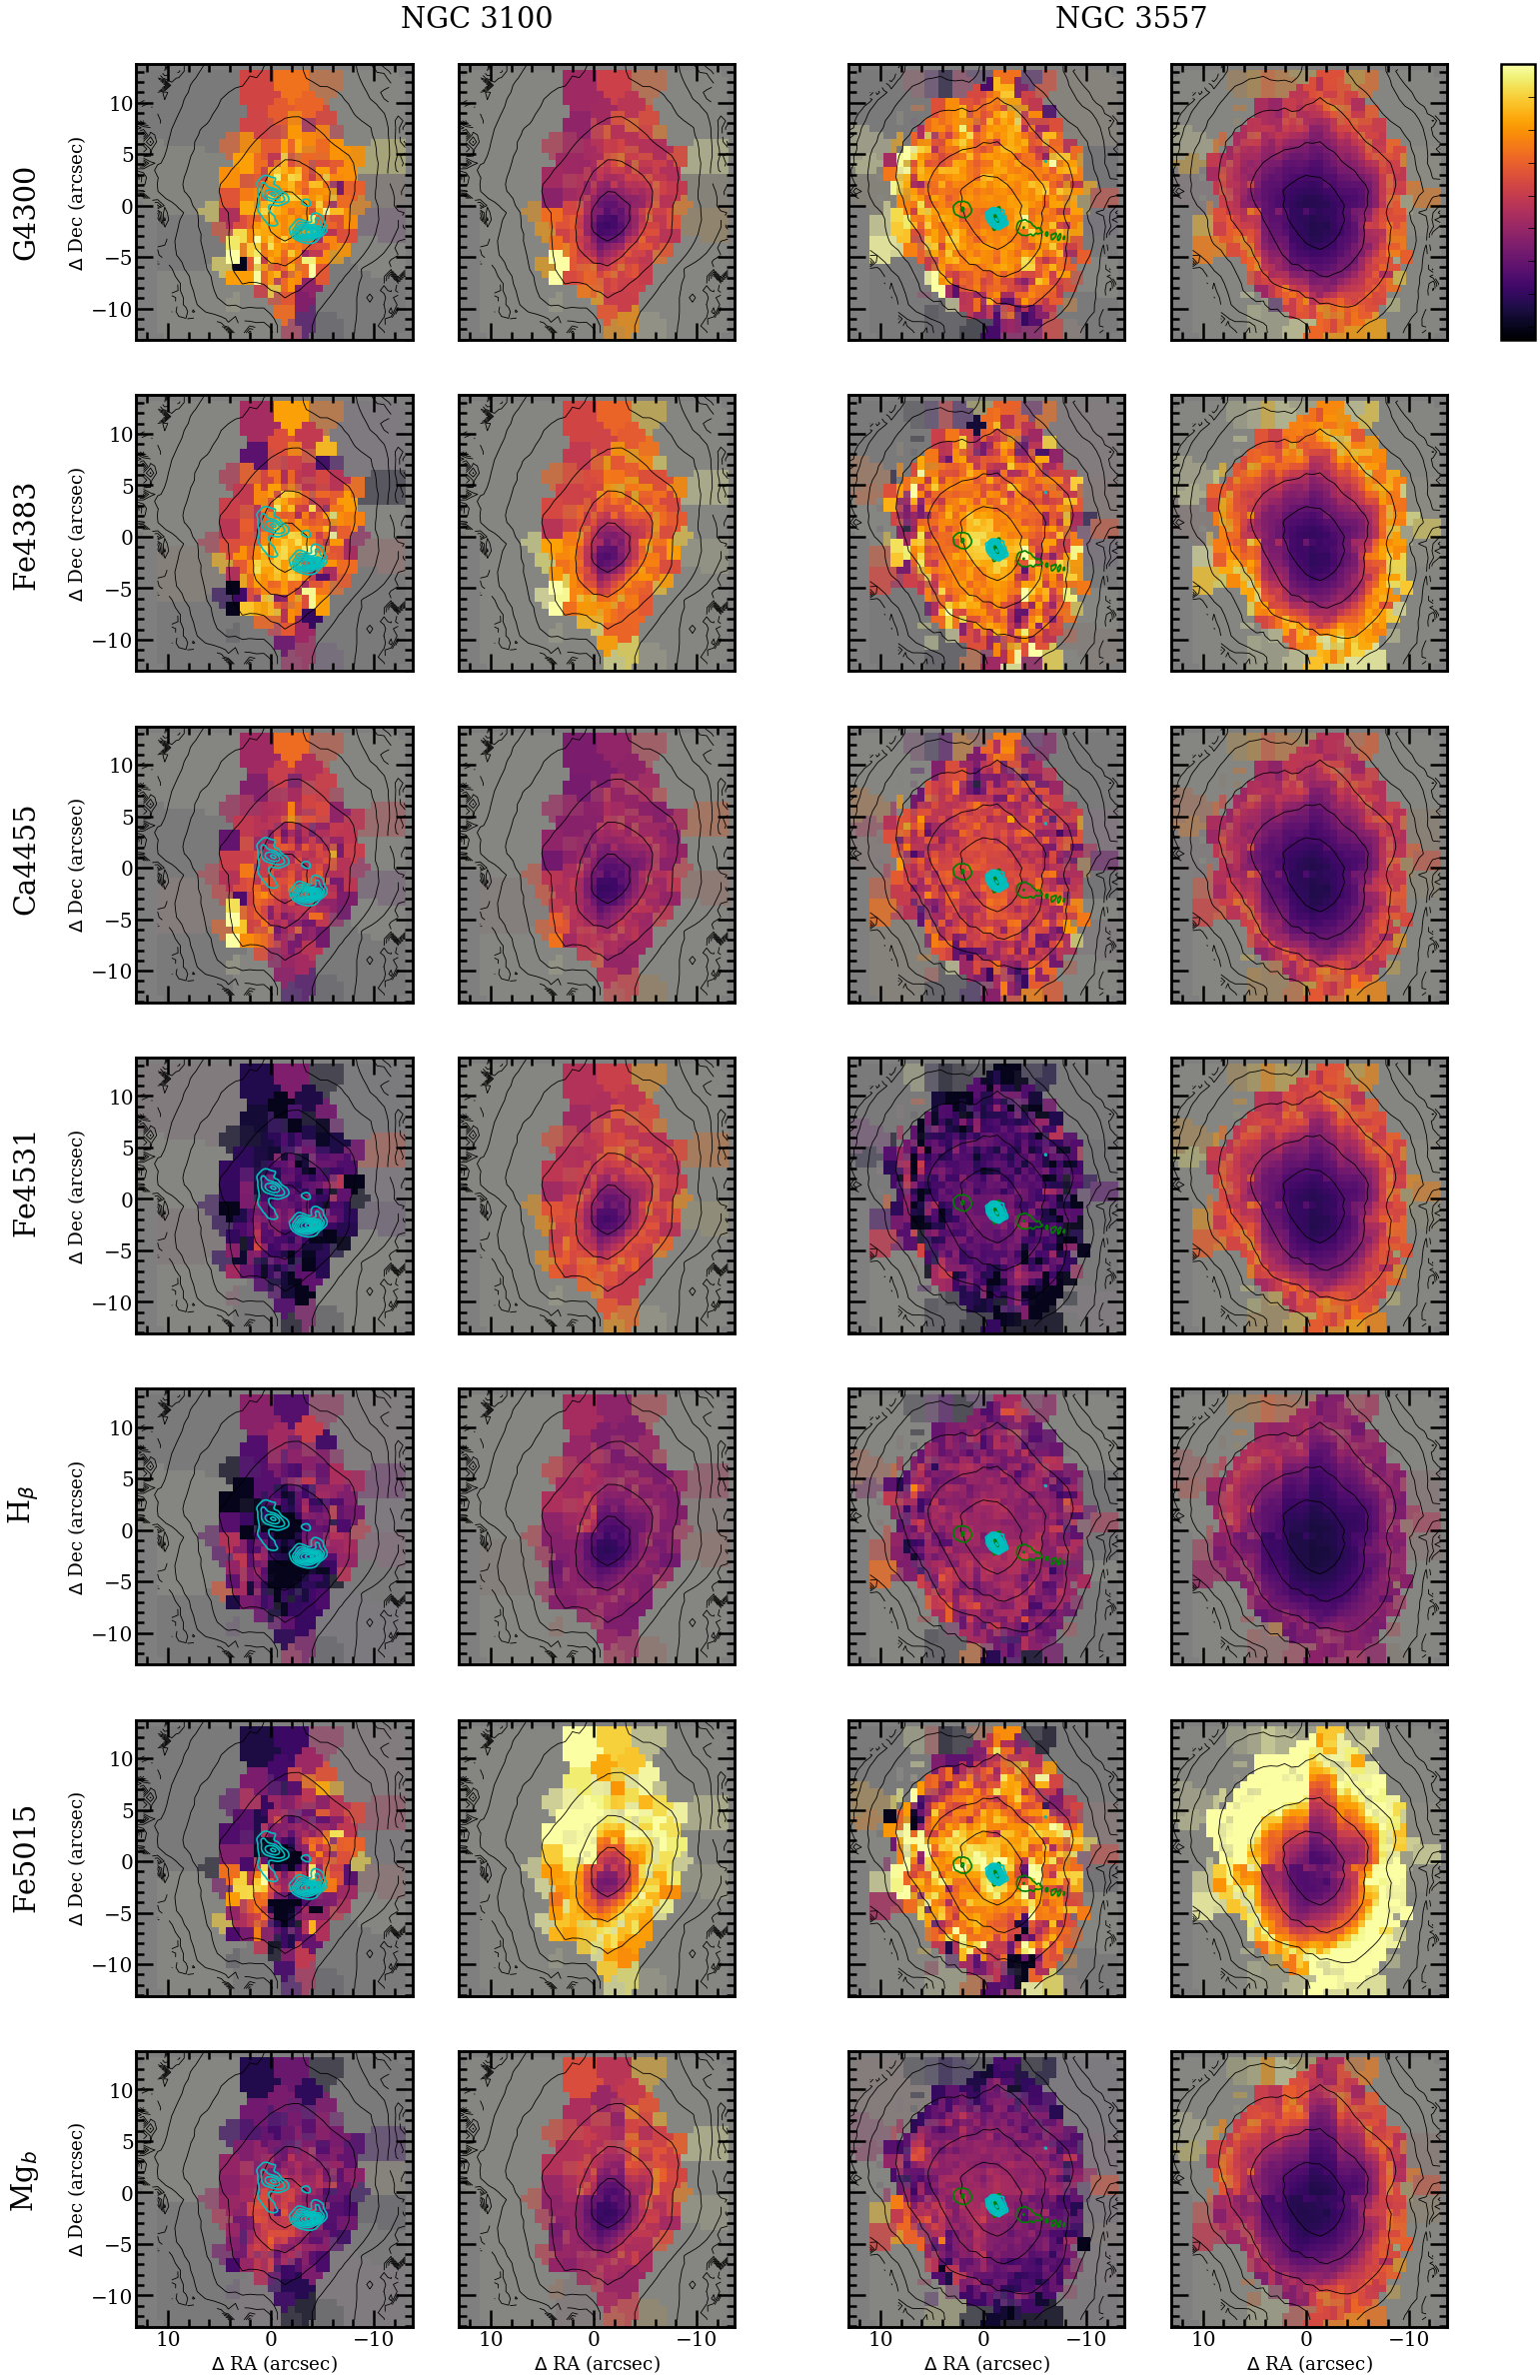
\includegraphics[height=0.94\textheight]{chapter4/vimos/abs4.png}
			\contcaption{\textit{Continued.}}% for NGC 3100 and NGC 3557}
		\end{figure}
		\begin{figure}
			\centering
			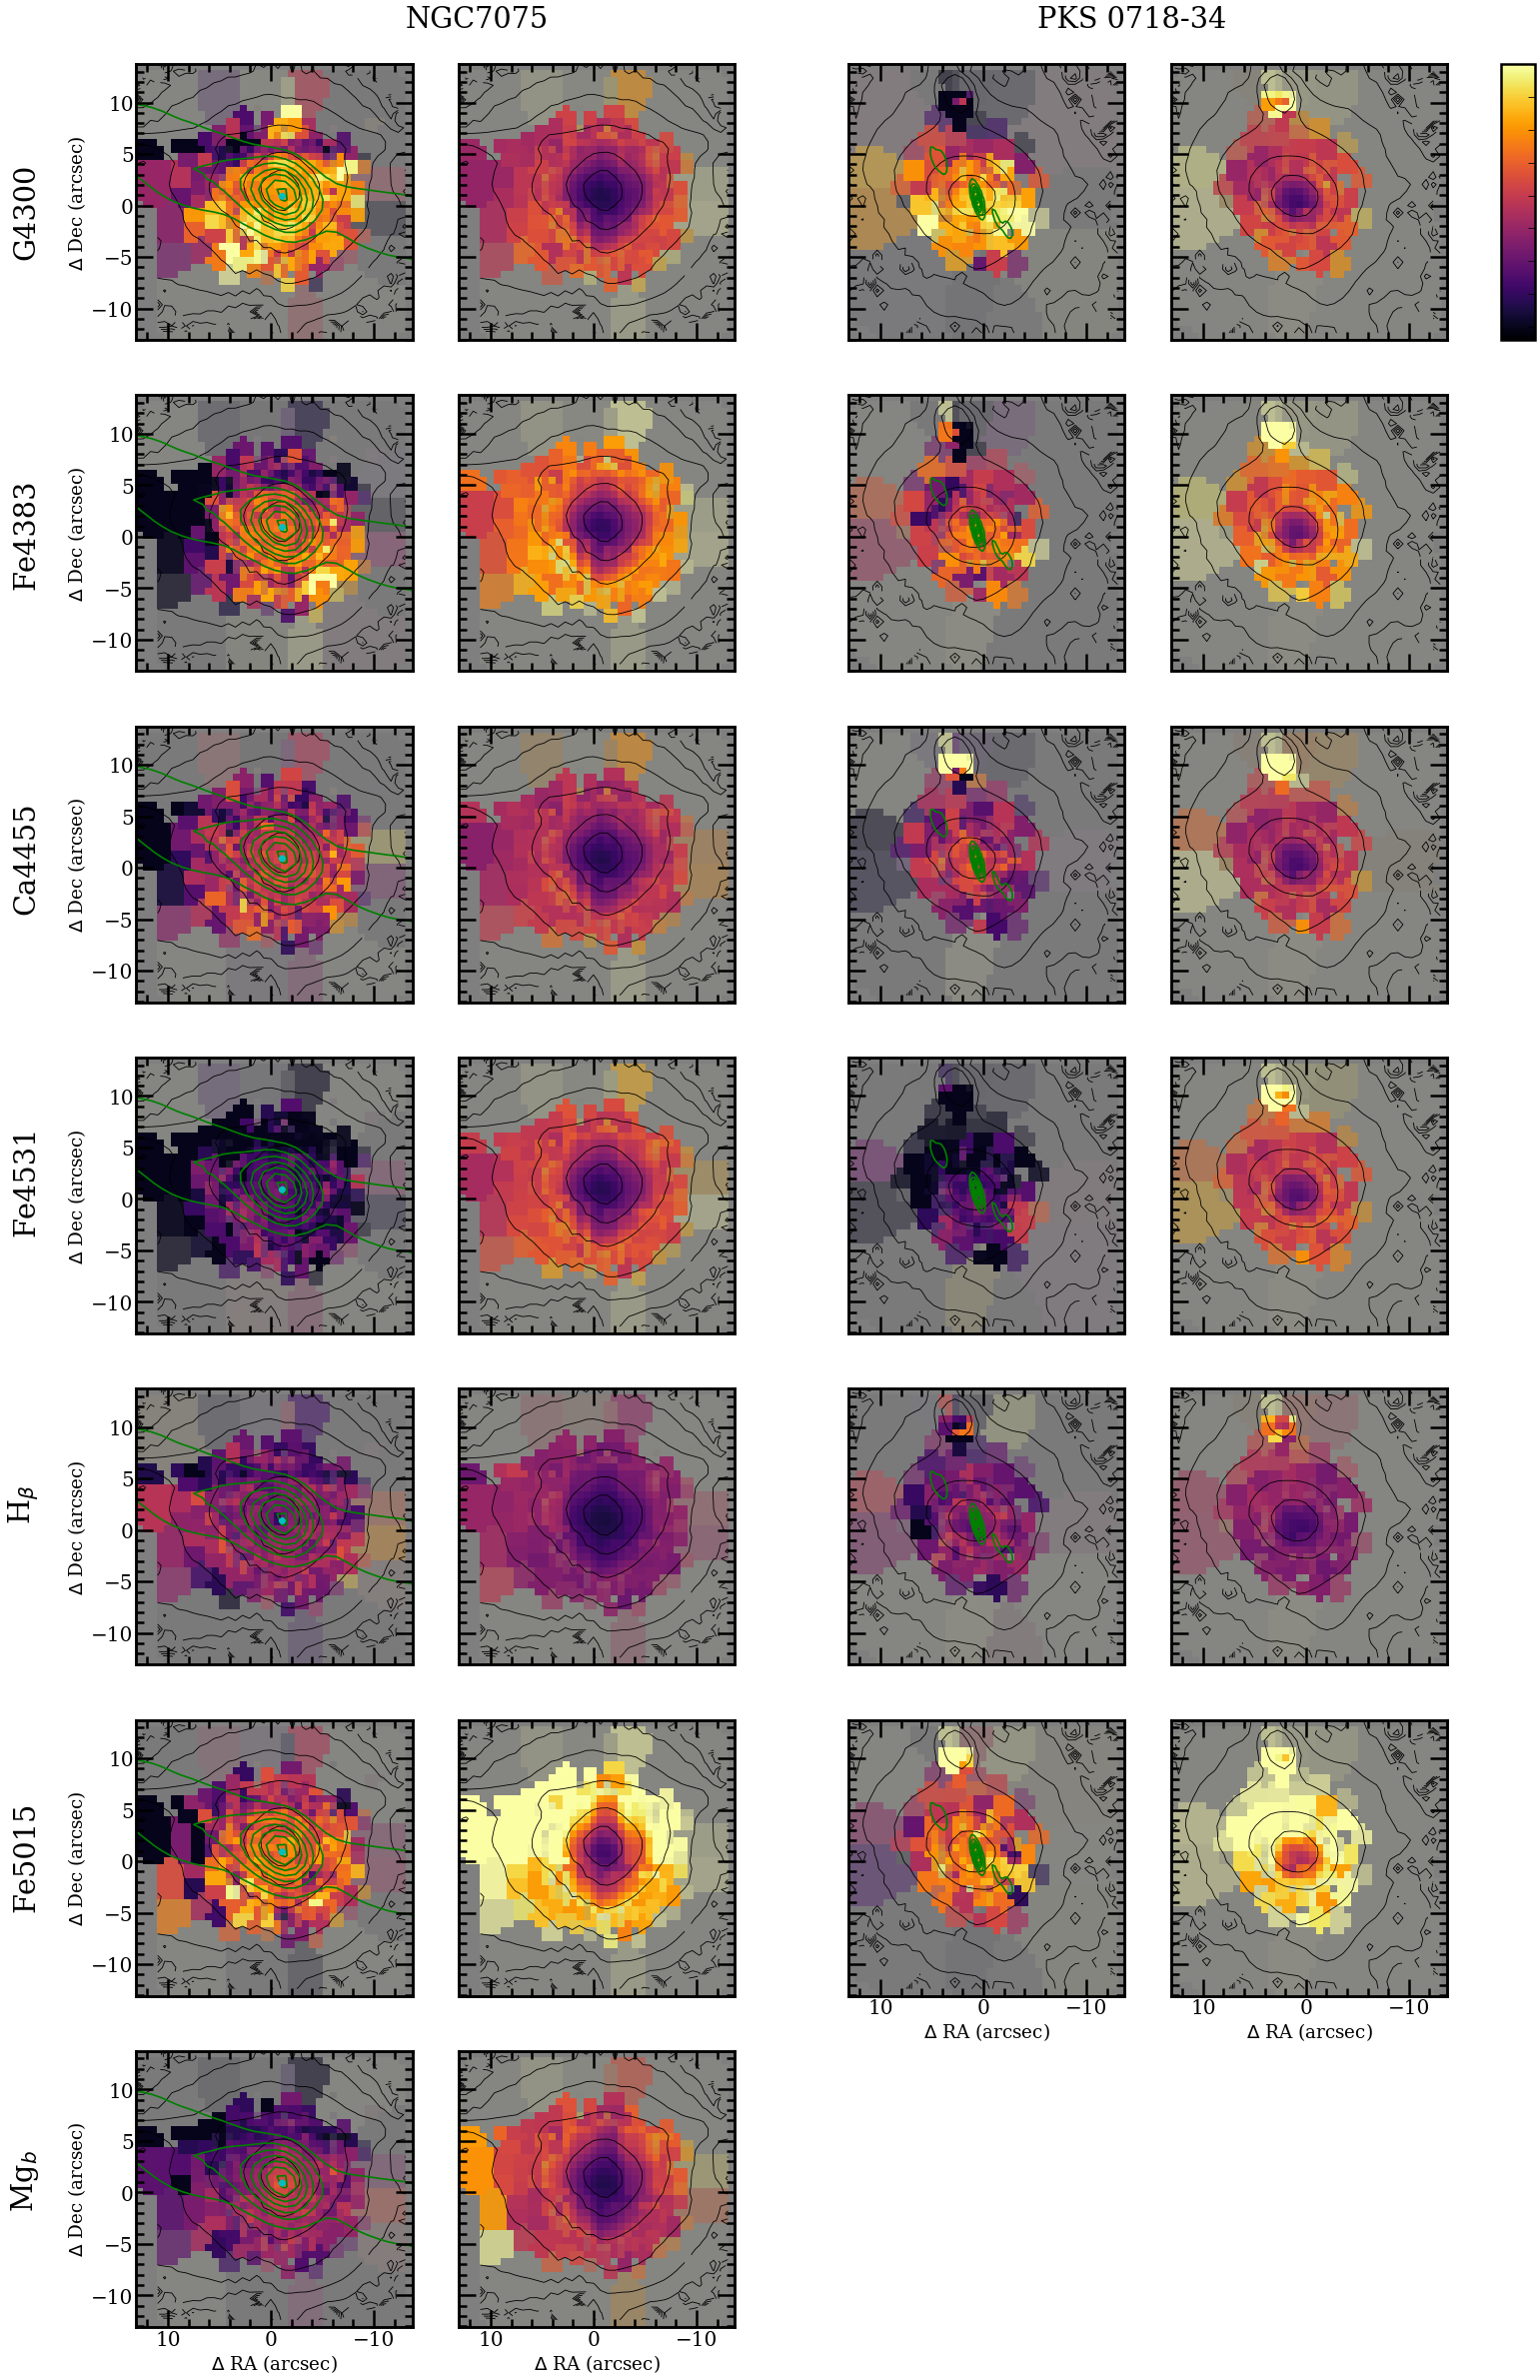
\includegraphics[height=0.94\textheight]{chapter4/vimos/abs5.png}
			\contcaption{\textit{Continued.}}% for NGC 7075 and PKS 718-34}
		\end{figure}

		\begin{figure}
			\centering
			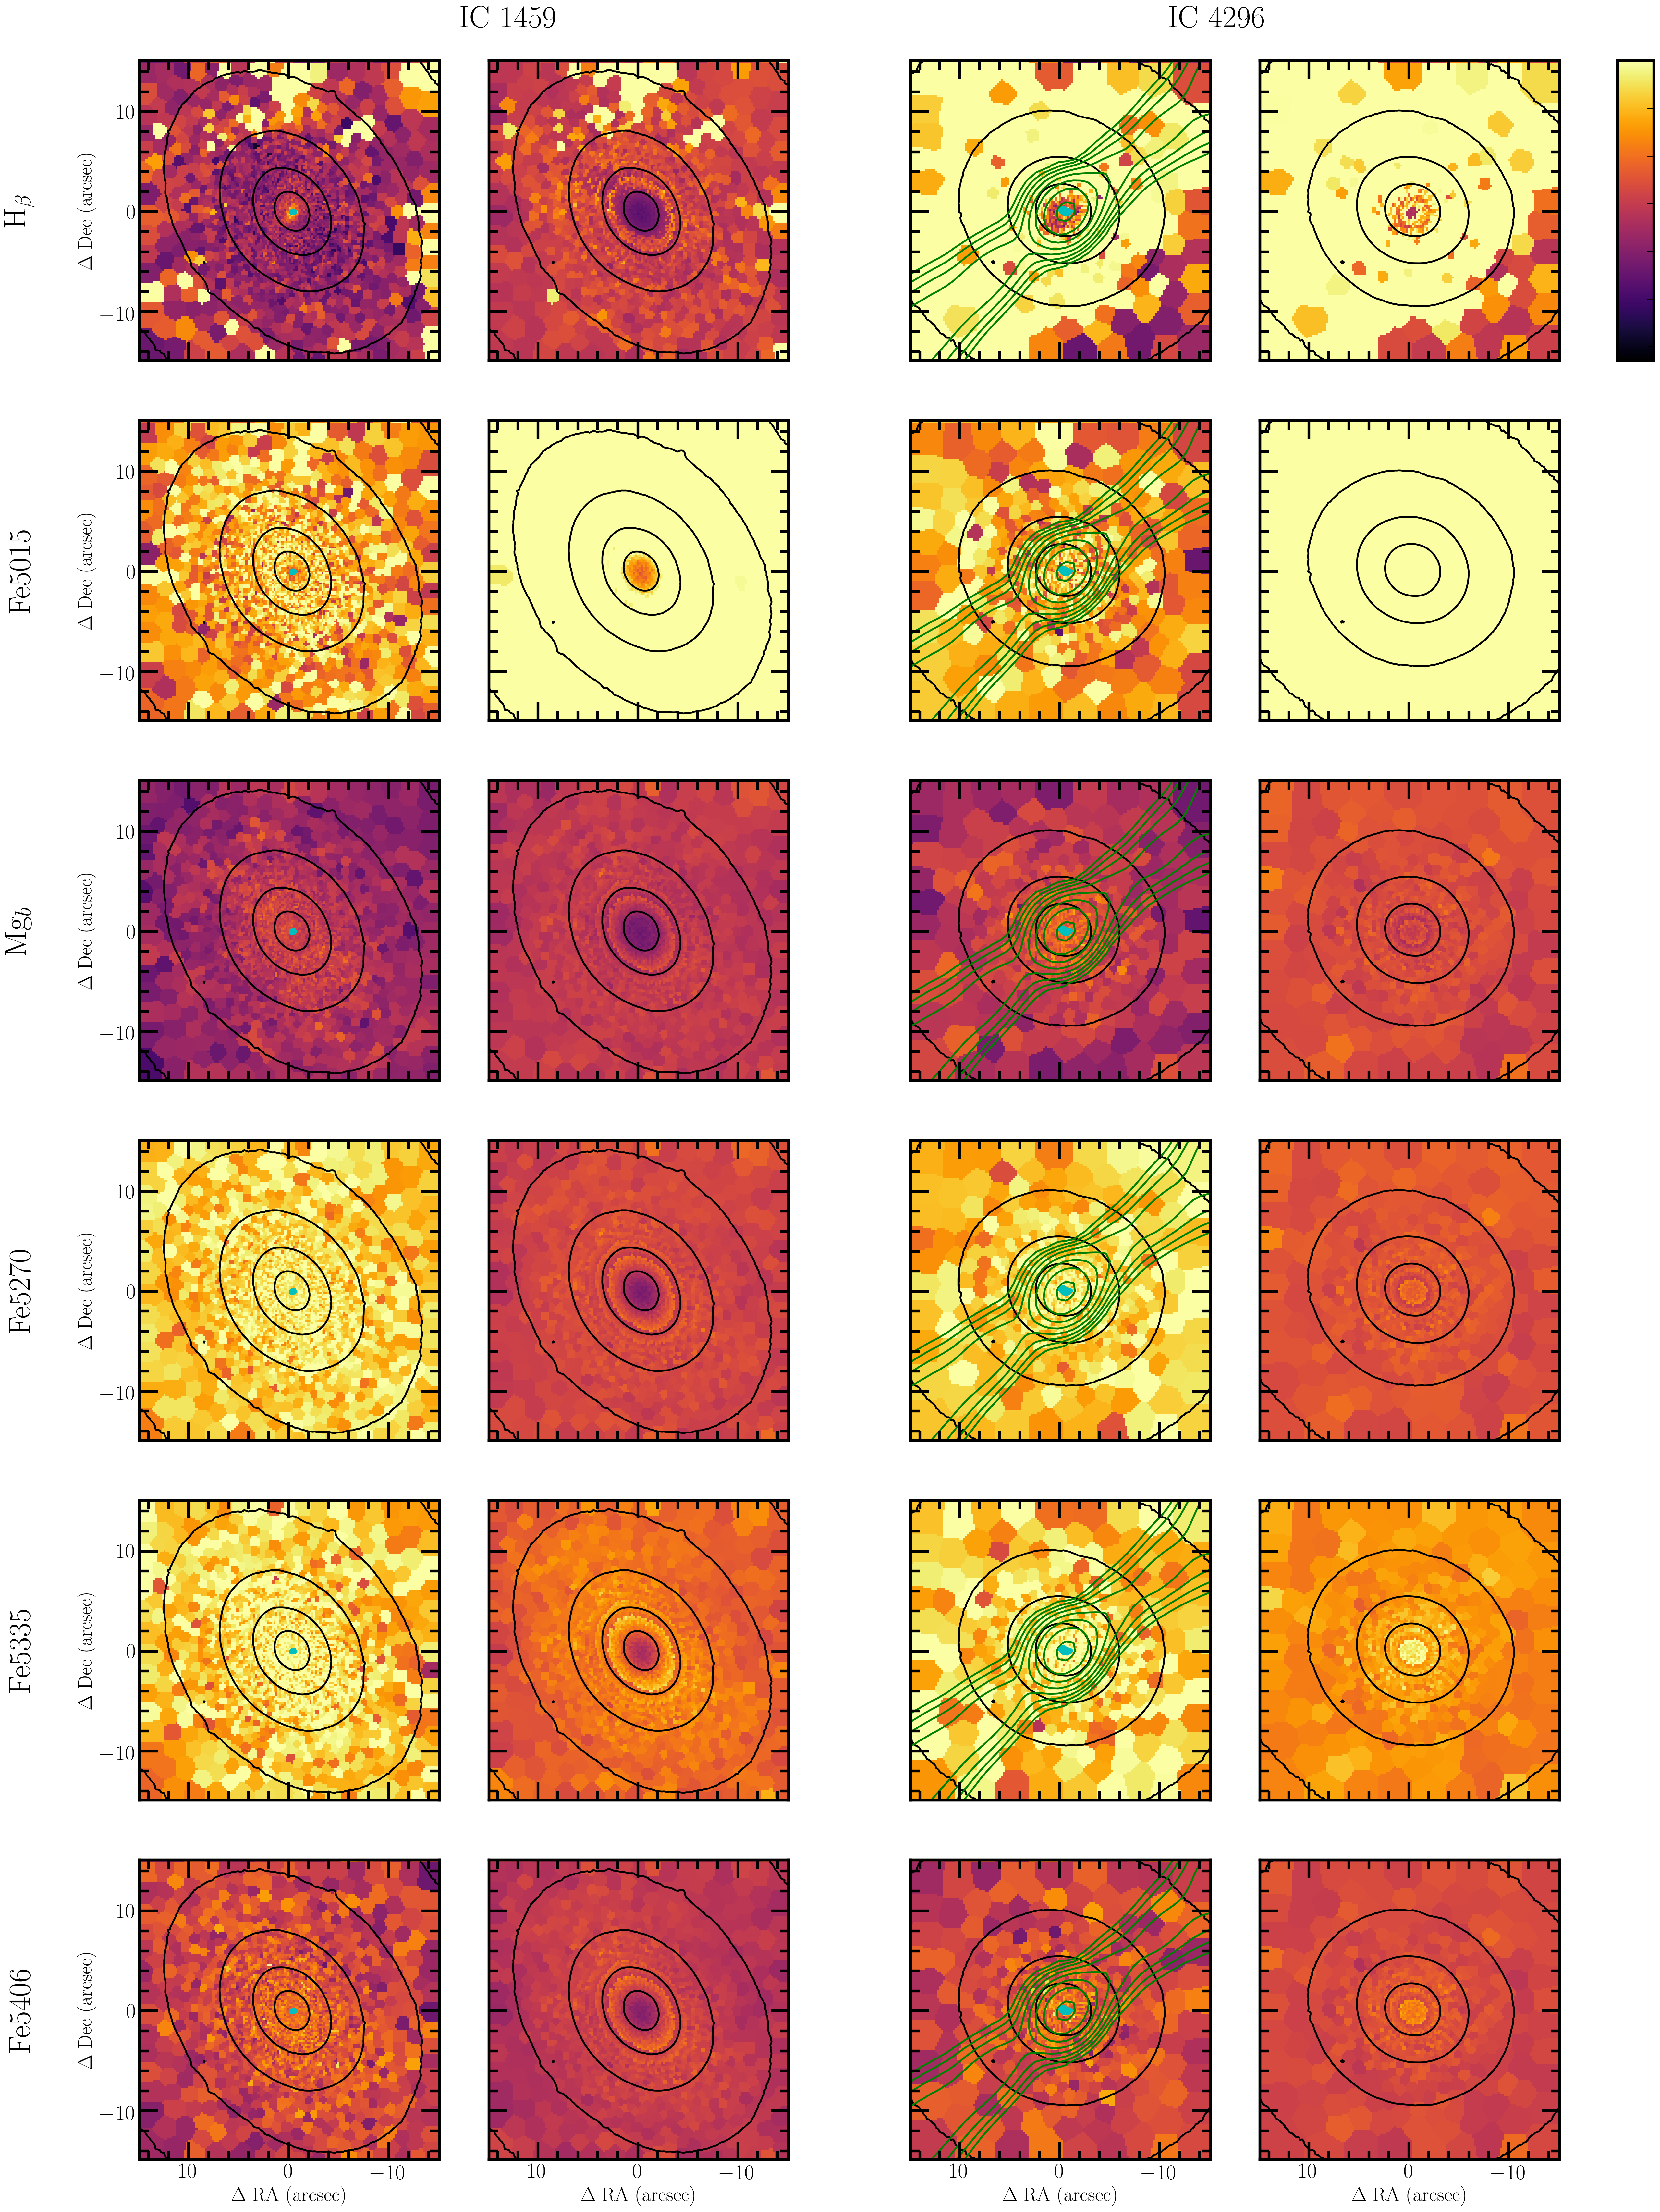
\includegraphics[height=0.81\textheight]{chapter4/muse/abs1.png}
			\caption[MUSE absorption line strength maps]{As Fig.\,\ref{fig:VIMOS_absorption} but for the MUSE absorption line strength maps. Limits on the colour scales are 0.5--3.5\,\AA\ for the H\,$\beta$, Fe5270, Fe 5335, Fe5406, Fe5709 and Fe5782 indices, 0--0.35\,mag for the TiO1 index, 0--0.1\,mag for the TiO2 index and 3--7\,\AA\ for all other indices. For the associated uncertainties the colour scale limits are 0--0.03\,mag for the TiO1 and TiO2 indices and 0--0.5\,\AA\ for all other indices.}
			\label{fig:MUSE_absorption}
		\end{figure}
		\begin{figure}
			\centering
			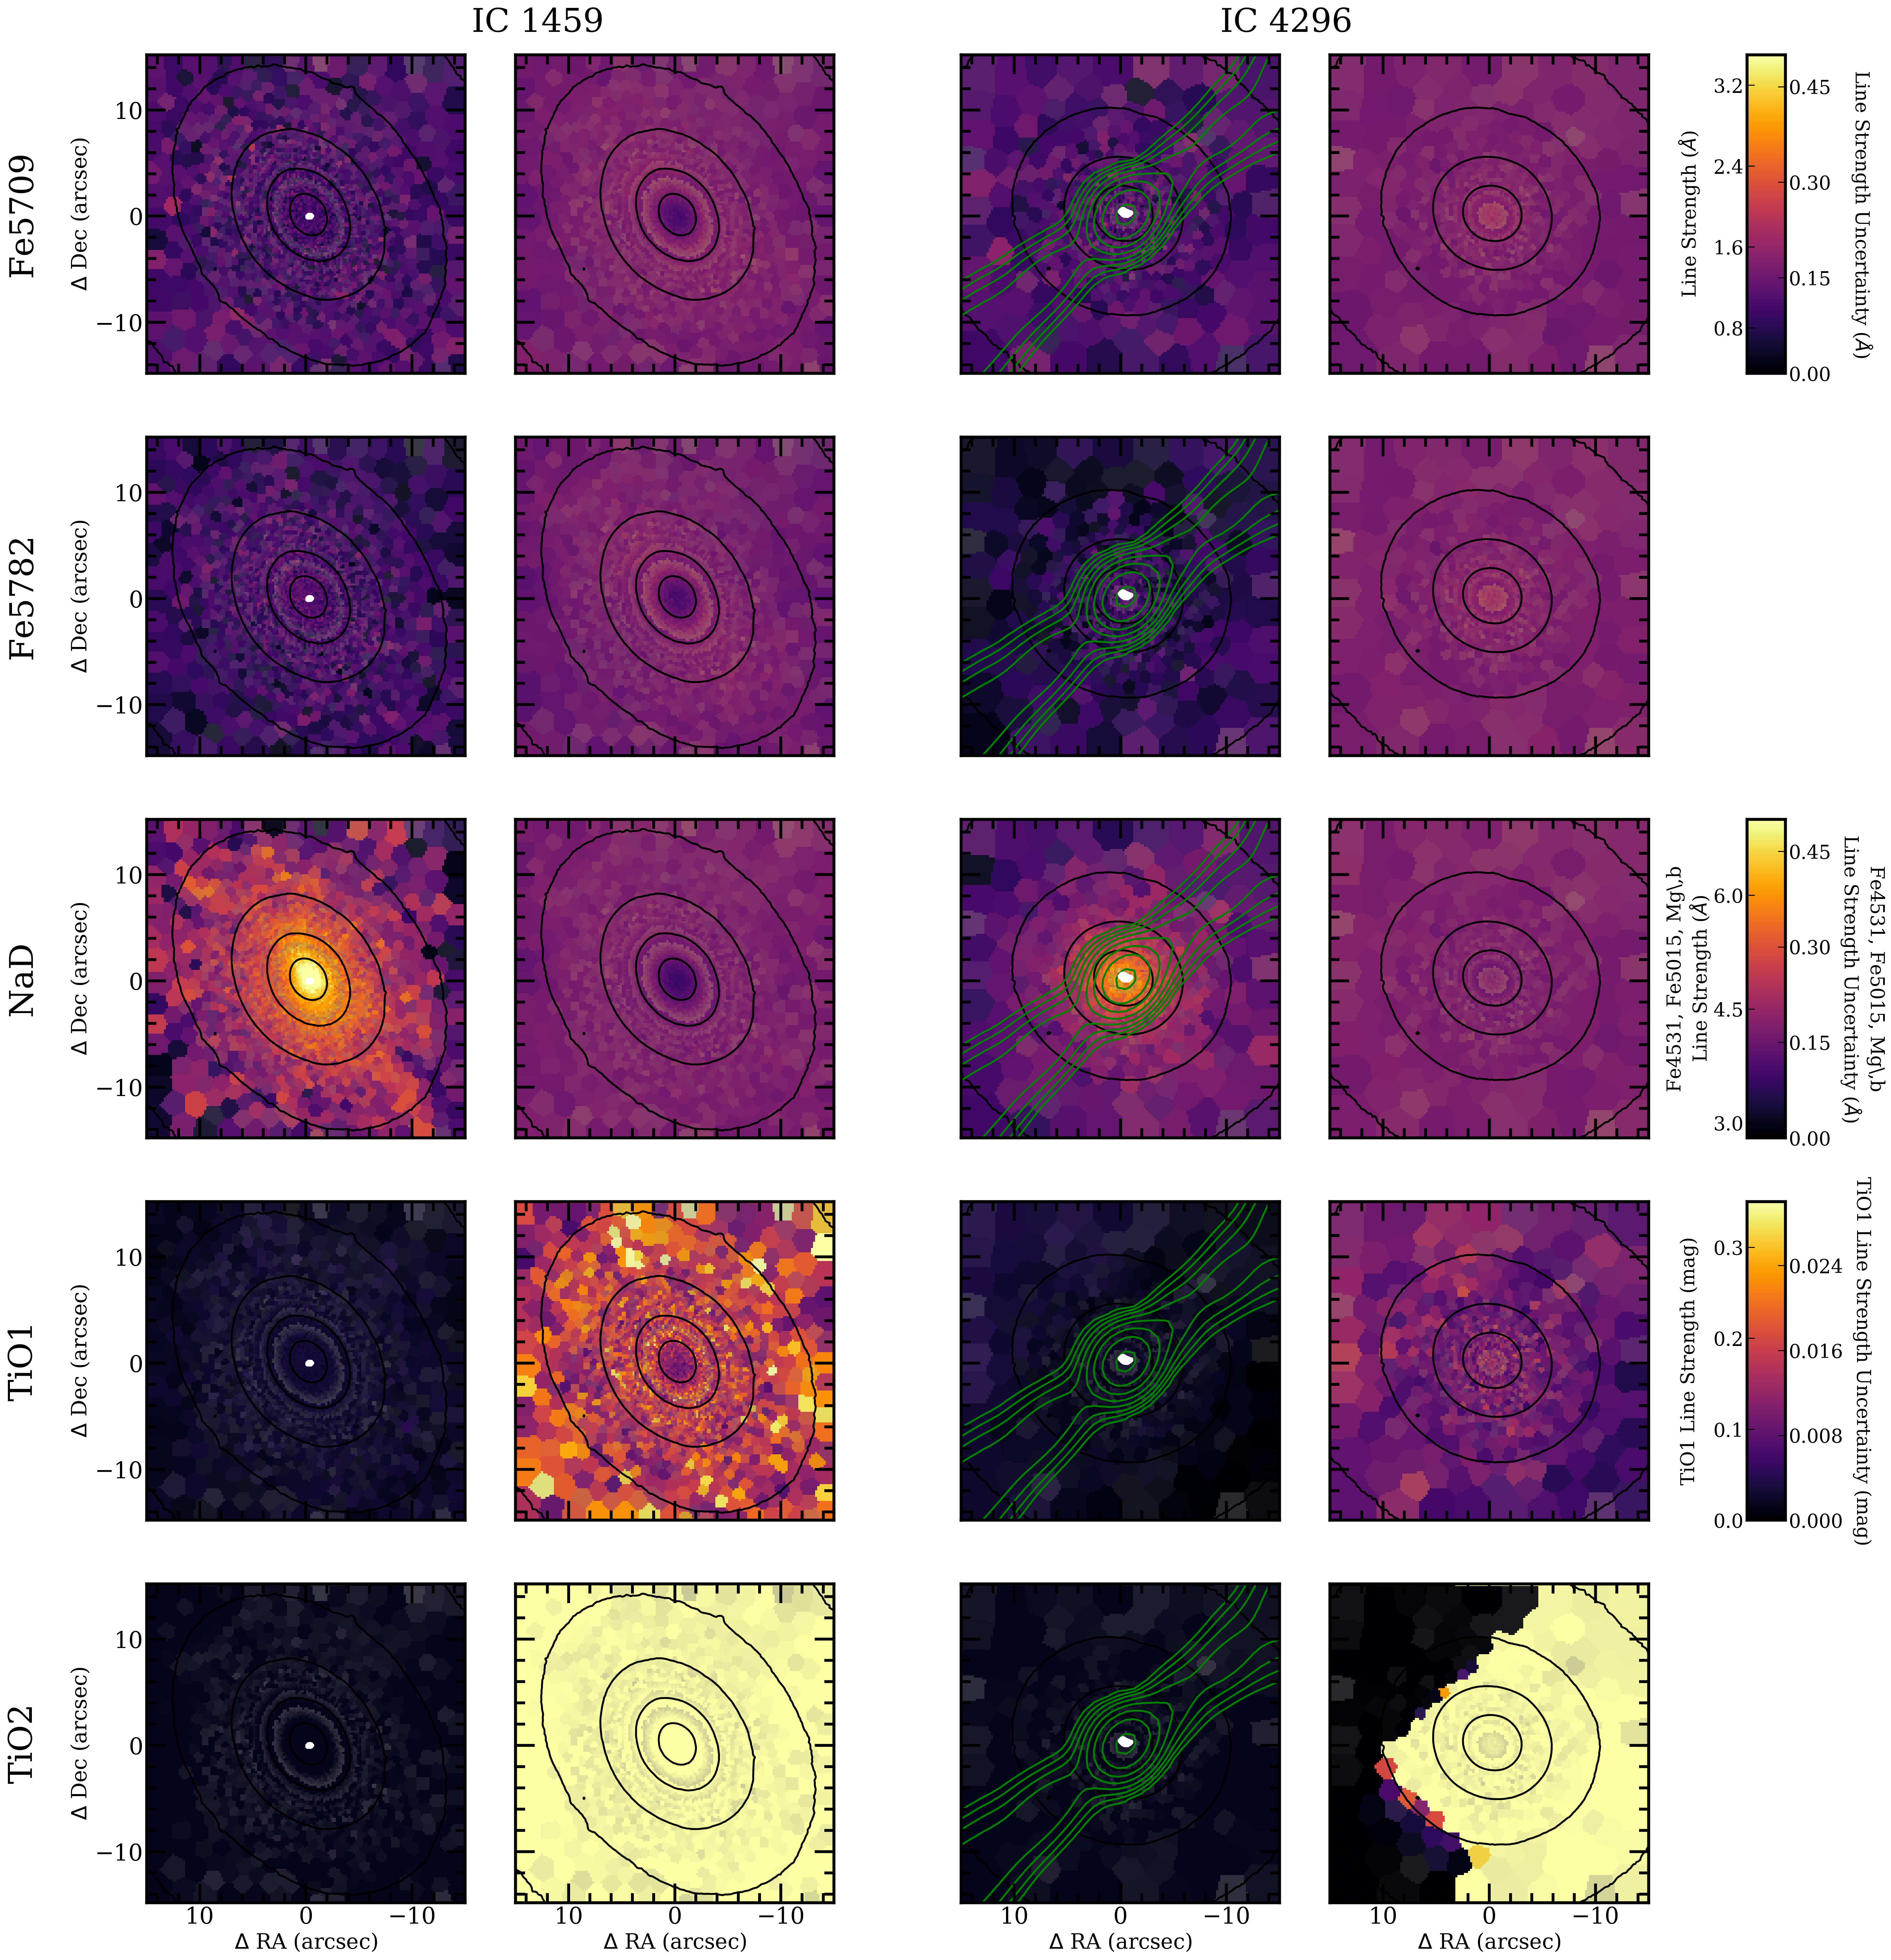
\includegraphics[height=0.67\textheight]{chapter4/muse/abs1b.png}
			\contcaption{\textit{Continued.}} %: From top to bottom: Fe5782, NaD, TiO1, TiO2. Plots are as in \ref{fig:VIMOS_stellar}. Limits on the colour scale are 0-9 \AA  for the line strengths and 0-1 \AA  for the uncertainties and 0-0.35 mag for TiO1 and TiO2 line strengths and 0-0.03 mag for the uncertainty in TiO1 and TiO2.}
		\end{figure}
		\begin{figure}
			\centering
			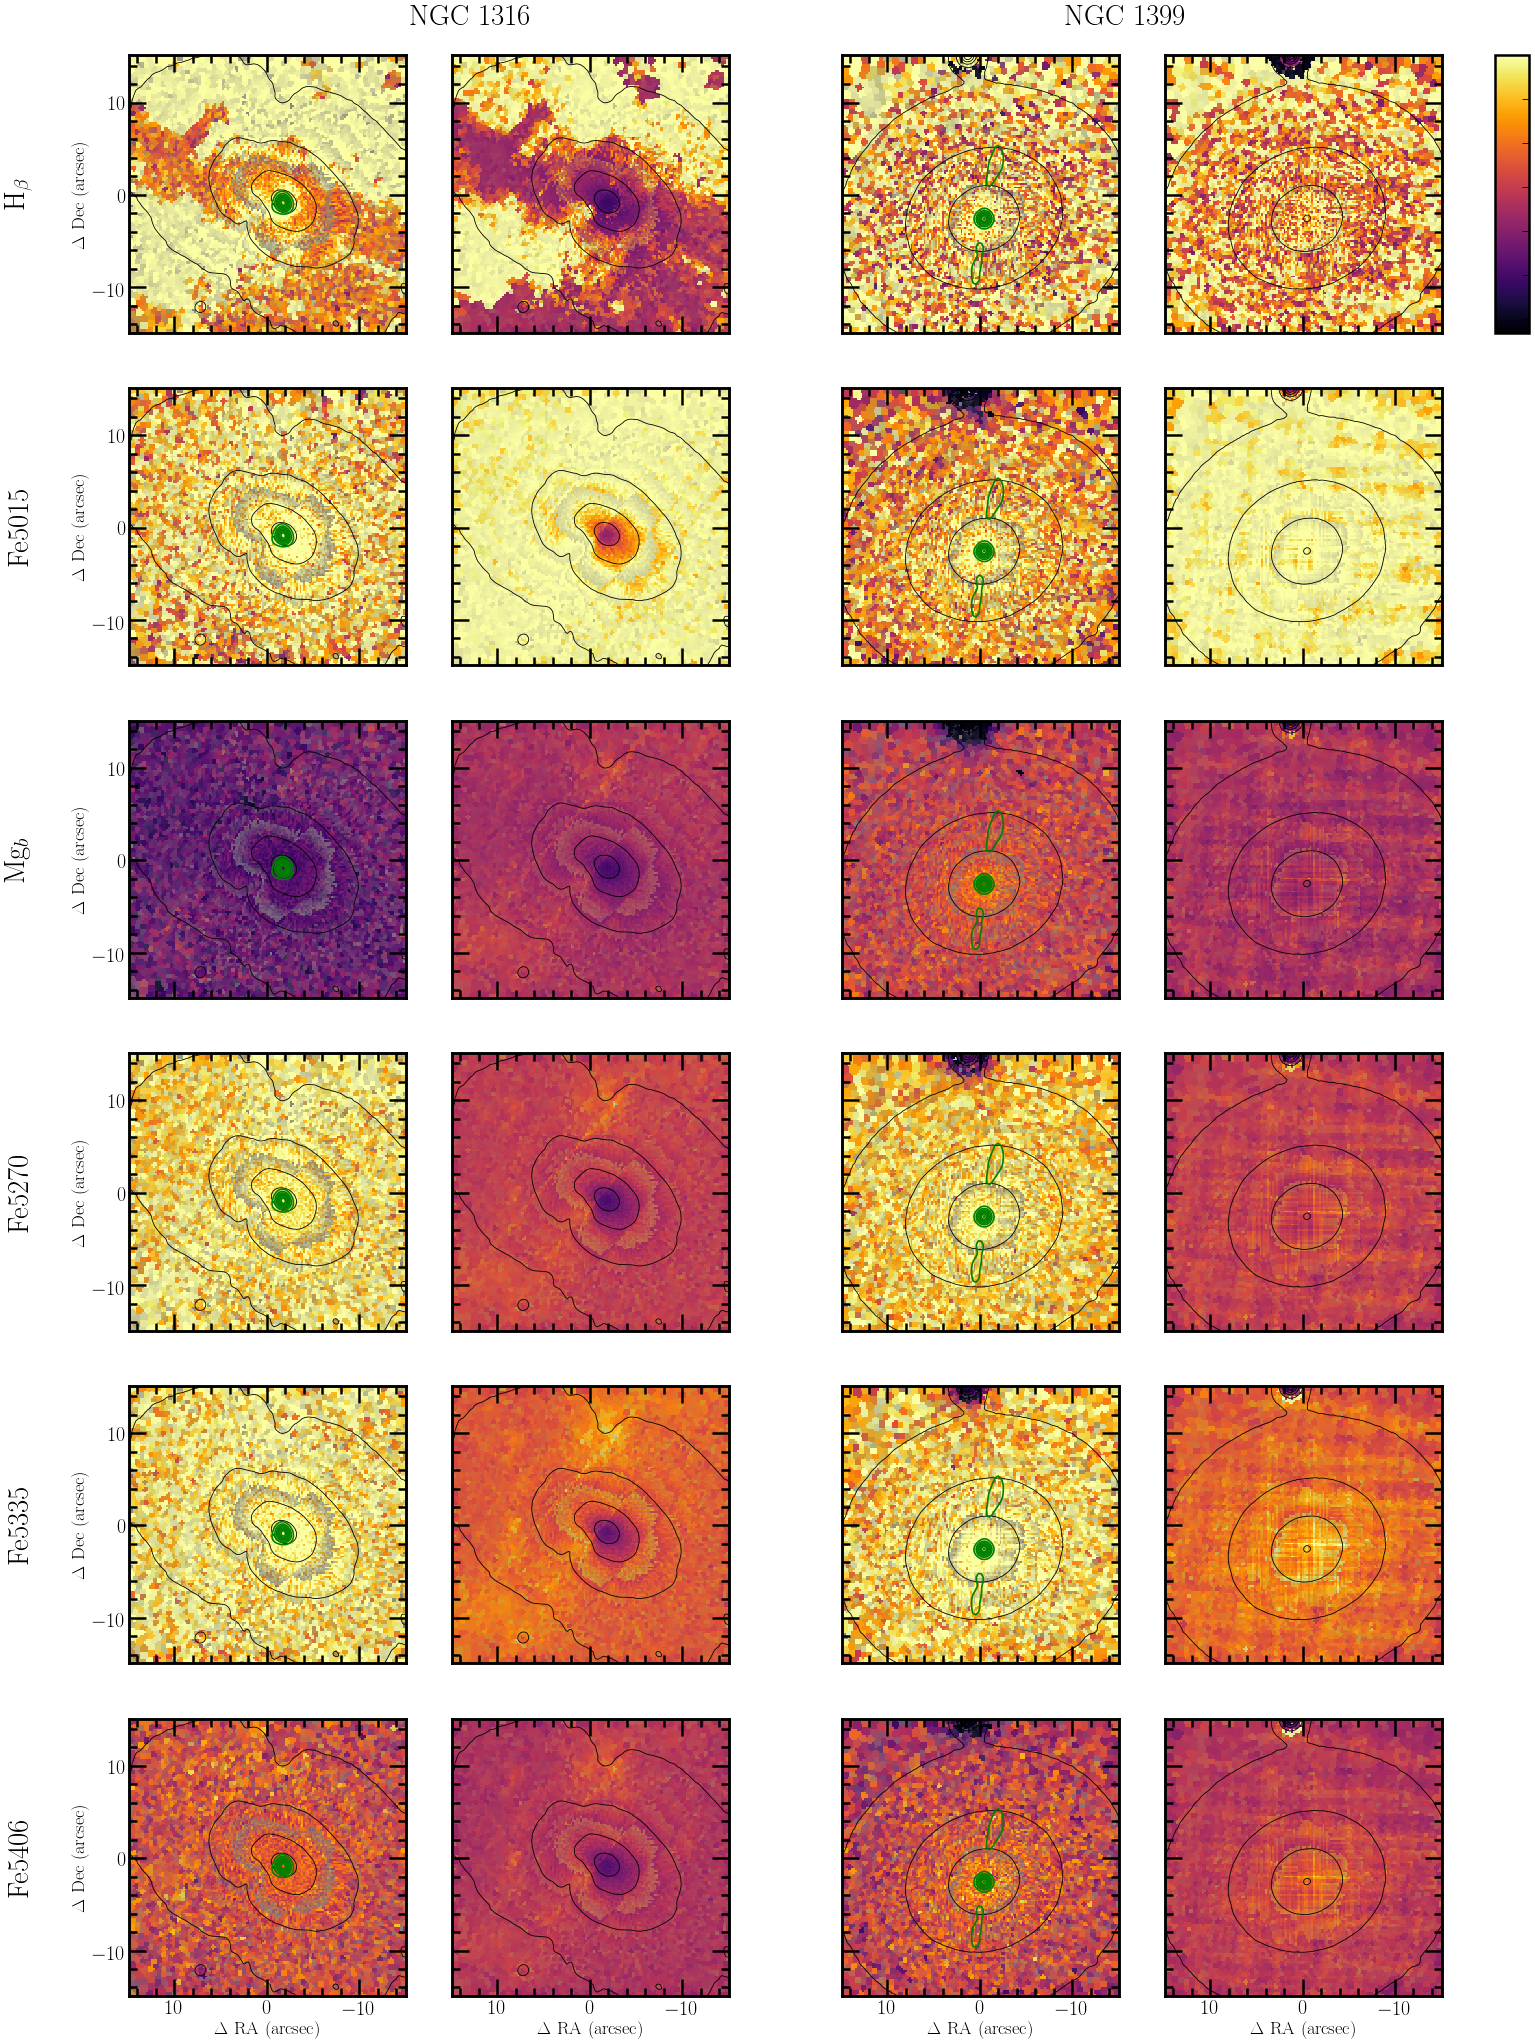
\includegraphics[height=0.81\textheight]{chapter4/muse/abs2.png}
			\contcaption{\textit{Continued.}}% for NGC1316 and NGC1399.}
		\end{figure}
		\begin{figure}
			\centering
			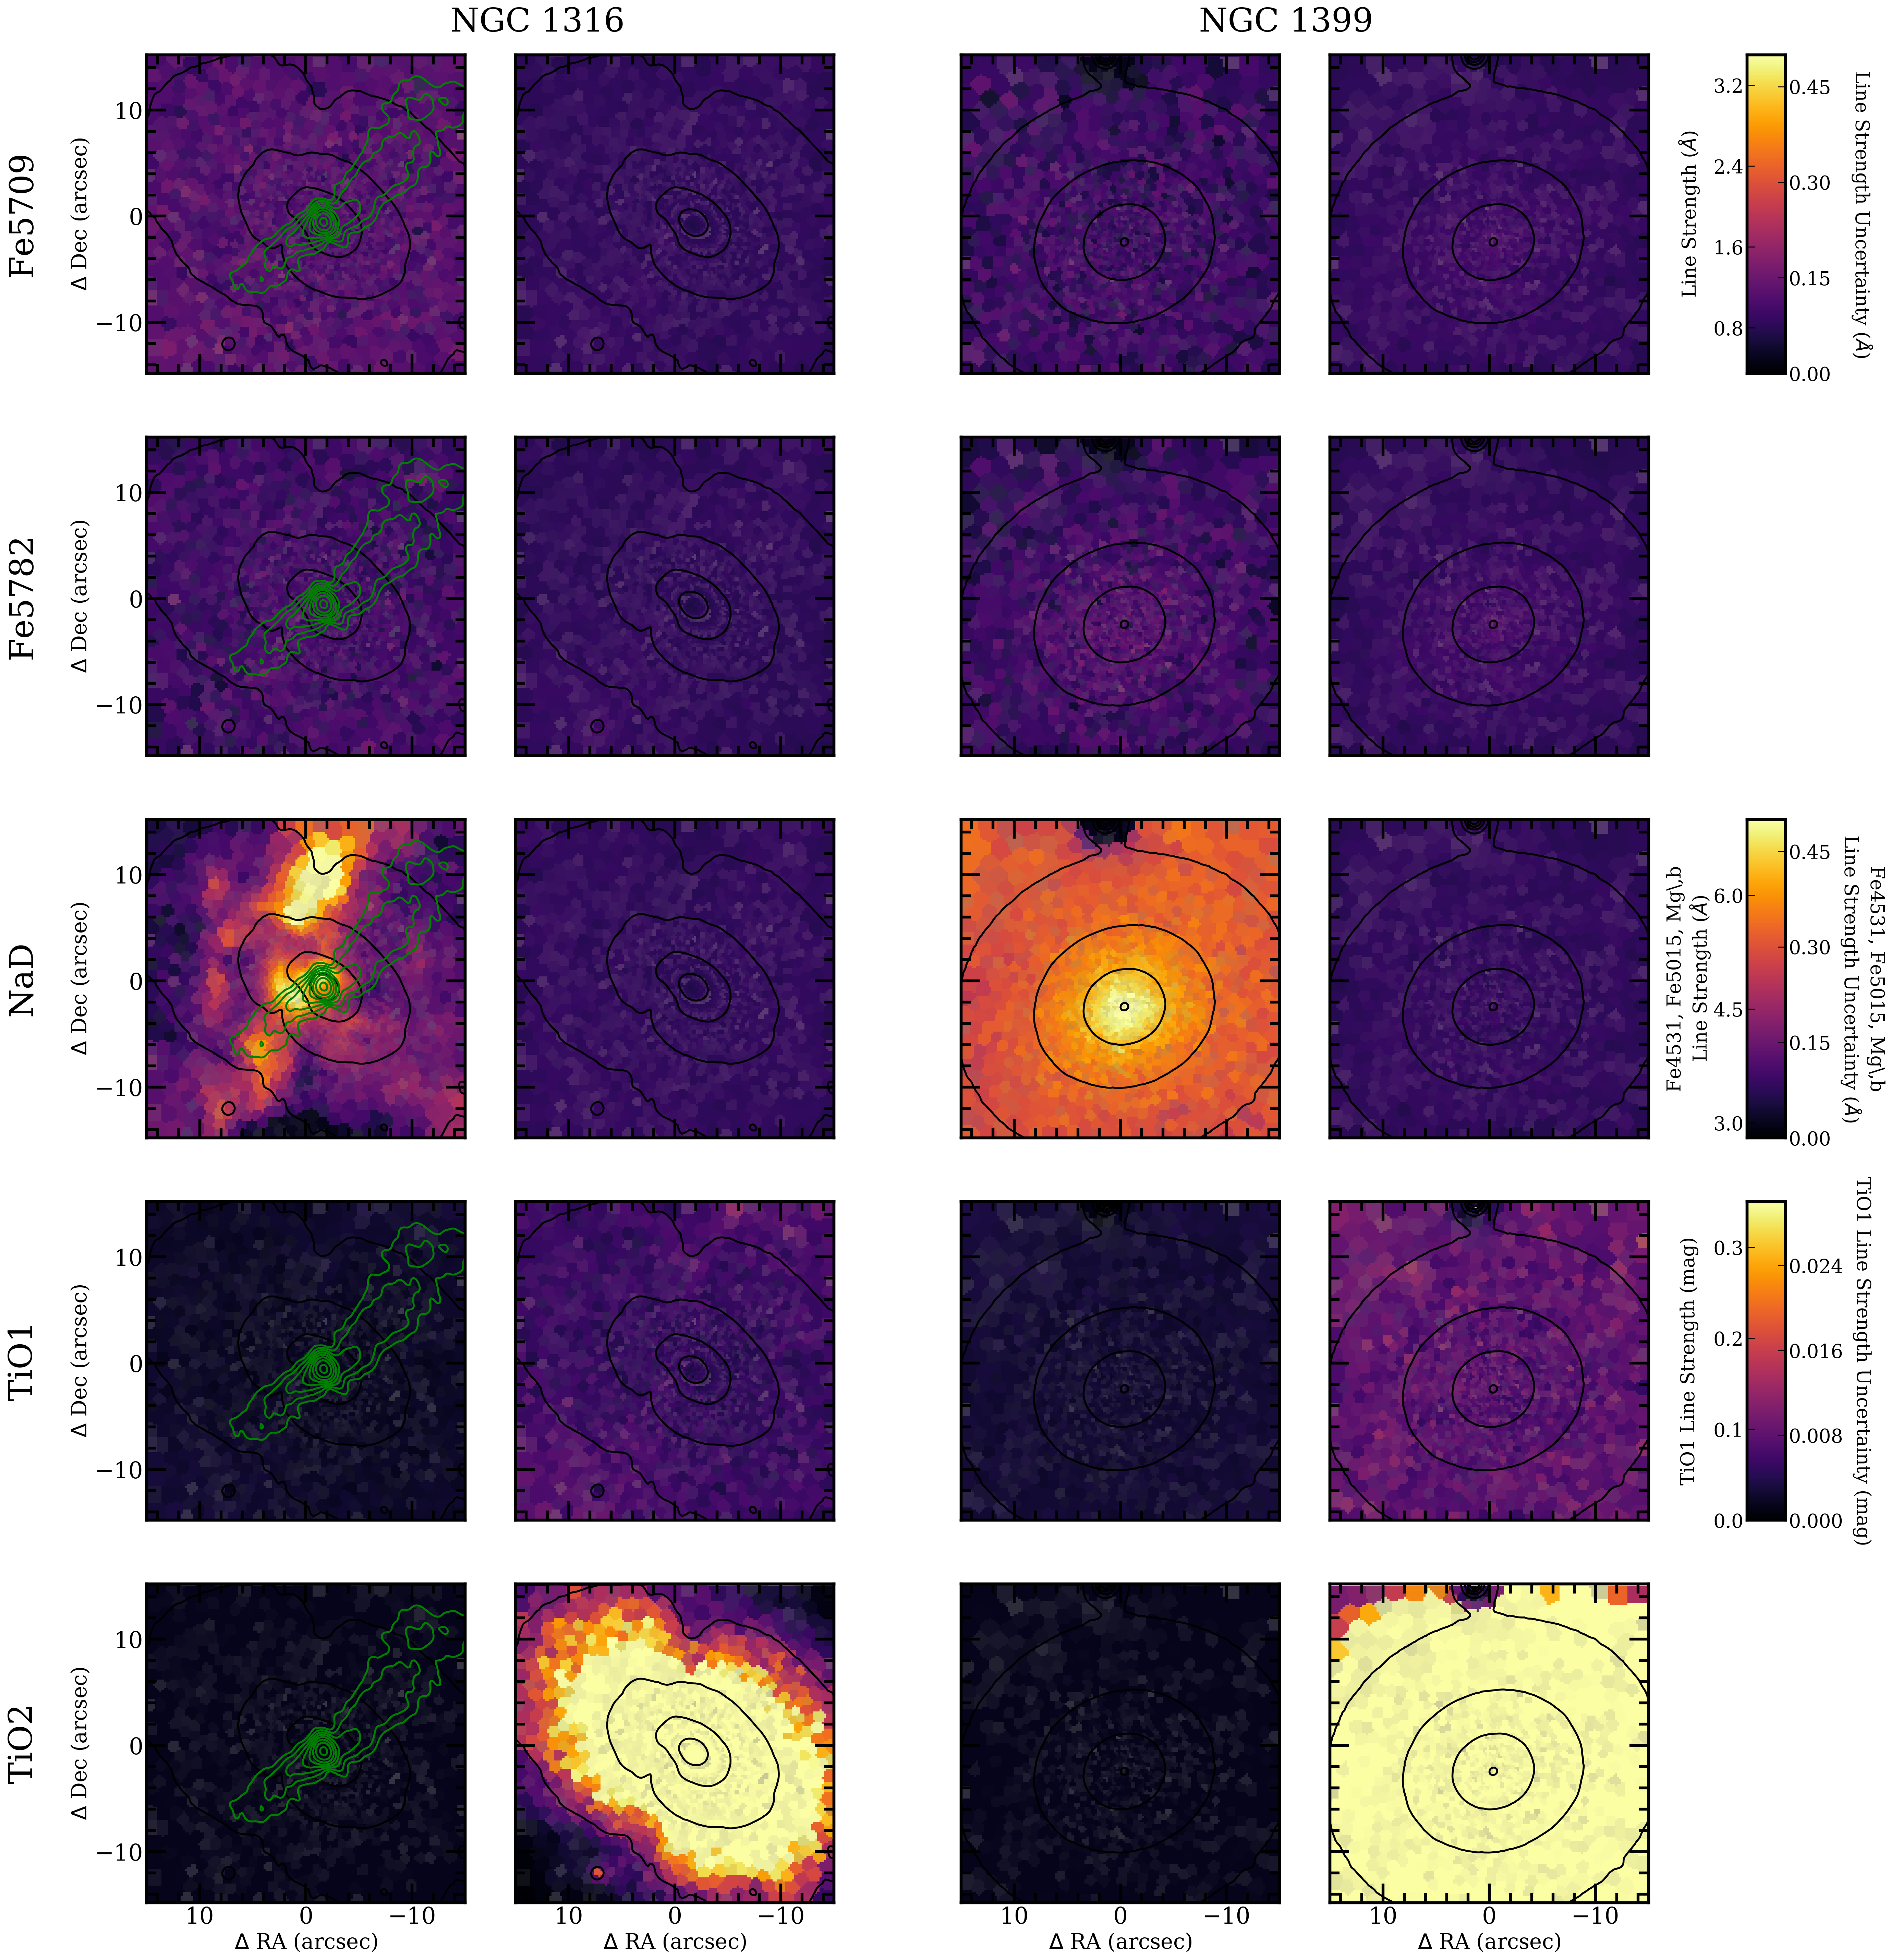
\includegraphics[height=0.67\textheight]{chapter4/muse/abs2b.png}
			\contcaption{\textit{Continued.}}% for NGC1316 and NGC1399.}
		\end{figure}

			We observe that most of our Southern sample show almost uniform, small H\,$\beta$ line strengths throughout a given galaxy, as well as slight central concentration in Fe, Ca4455 and Mg\,b index maps. NGC 612 is the exception to these trends, with large H\,$\beta$ line strengths, particularly along the dust lane and larger gradients in Fe and Ca4455 (Mg\,b is redshifted out of the spectral range of VIMOS for this galaxy; see Section \ref{secNGC612}). The MUSE derived maps also show a significantly central concentration in the NaD index. The NaD feature is thought to be significantly increased by absorption from the interstellar medium (ISM) if present \citet[e.g.][]{Phillips1993, Bergmann2009}, a concept consistent with the apparent tracing of the dust lane within NGC 1316 of the NaD line strength. Like NGC 612, NGC 1316 also has large H\,$\beta$ line strengths, again with the highest values along the dust lane. 

		\subsubsection{Mg -- $\sigma$ relation}
			\label{subsubssec:Mgsigma}
			The definition of the Mg$_2$ absorption line index (blue continuum: 4895.125--4957.625\,\AA, index bandpass: 5154.125--5196.625\,\AA\ and red continuum: 5301.125--5366.125\,\AA) has overlapping bandpasses with the Mg\,b index, but includes the MgH molecular absorption line, and is hence considered a molecular index and is measured in magnitude units. It was \citet{Bender1993} who first noticed the unusually tight relationship between the global Mg$_2$ absorption line strength and central velocity dispersion, $\sigma_0$, in elliptical galaxies. They also noticed that residuals appeared to be intrinsic as they had a near Gaussian shape about the median values, but did not seem to be correlated to any other galaxy property. 

			Since part of the red continuum band of the Mg$_2$ index is outside of the spectral range of VIMOS, we instead use the Mg\,b index. \citet{Ziegler1997} show there is a linear relationship between Mg\,b and Mg$_2$, with a gradient of 14.3--15.5\,mag\,\AA$^{-1}$\ depending on metallicity. We thus use Mg\,b as a proxy for Mg$_2$. 

			Using an aperture with a radius of 2 arcsec on each datacube, we measure $\sigma_0$ and Mg\,b at a spectral resolution of 8.4\,\AA full-width half-maximum (FWHM; see Table \ref{tab:globalMg} and points in Fig.\,\ref{fig:globalMg}). The best-fitting linear relationship (found using \textsc{lts\_linefit} by \citet{Cappellari2013}) has a gradient of $2.3 \pm 0.5 \,\mathrm{\AA/\log(km \, s^{-1})}$ (solid black line in Fig.\,\ref{fig:globalMg}) with an intrinsic scatter of $0.12 \pm 0.10 \, \mathrm{\AA}$. 

			This is in very good agreement with the gradient found by \citet{Ziegler1997} for a sample of elliptical galaxies within Virgo and Coma using data from \citet{Dressler1987} of $2.5\,\mathrm{\AA/\log(km \, s^{-1})}$ (shown as the blue dotted line in Fig.\,\ref{fig:globalMg}), with an intrinsic scatter of 0.16\,\AA\ for galaxies with $\log \sigma_0 \geqslant 2.3$. However, Fig.\,\ref{fig:globalMg} shows there is a considerable offset of $\approx0.75\,\mathrm{\AA}$ between our best-fitting line (solid line) and the best-fitting line (dashed line) from \citet{Ziegler1997}. Individual measurements for each galaxy are given in table \ref{tab:globalMg}.

			\begin{table}
				\centering
			\begin{threeparttable}
				\caption{The Mg\,b index and velocity dispersion within 2 arcsec.}
				\label{tab:globalMg}
				\begin{tabular}{l c c}
					\hline
					\hline
					Galaxy 	& Mg\,b & $\sigma_0$ \\
							& \AA 	& km s$^{-1}$ \\
					\hline
					ESO 443-G024 & $4.43 \pm 0.08$ & $332.4 \pm 1.6$ \\
					IC 1459 	& $4.67 \pm 0.03$ & $292.7 \pm 0.6$ \\
					IC 1531 	& $3.74 \pm 0.06$ & $222.9 \pm 1.3$ \\
					IC 4296		& $4.57 \pm 0.13$ & $361.7 \pm 2.1$ \\
					NGC 612 	& --   			  & $228.5 \pm 1.9$ \\
					NGC 1316 	& $3.45 \pm 0.08$ & $233.3 \pm 1.5$ \\
					NGC 1399 	& $4.57 \pm 0.13$ & $319.1 \pm 2.1$ \\
					NGC 3100 	& $4.36 \pm 0.05$ & $214.2 \pm 1.1$ \\
					NGC 3557 	& $4.15 \pm 0.03$ & $280.4 \pm 0.9$ \\
					NGC 7075 	& $4.45 \pm 0.07$ & $258.7 \pm 1.9$ \\
					PKS 718-34  & -- 		      & $258.7 \pm 1.9$ \\
					\hline
					\hline
				\end{tabular}
				\begin{tablenotes}
				\footnotesize
				\note NGC 612 and PKS 718-34 have a redshift which shifts the Mg\,b feature outside of the wavelength range of VIMOS.
				\end{tablenotes}
			\end{threeparttable}
			\end{table}

% Is the captions still true? Is it consistant?
			\begin{figure}
				\centering
				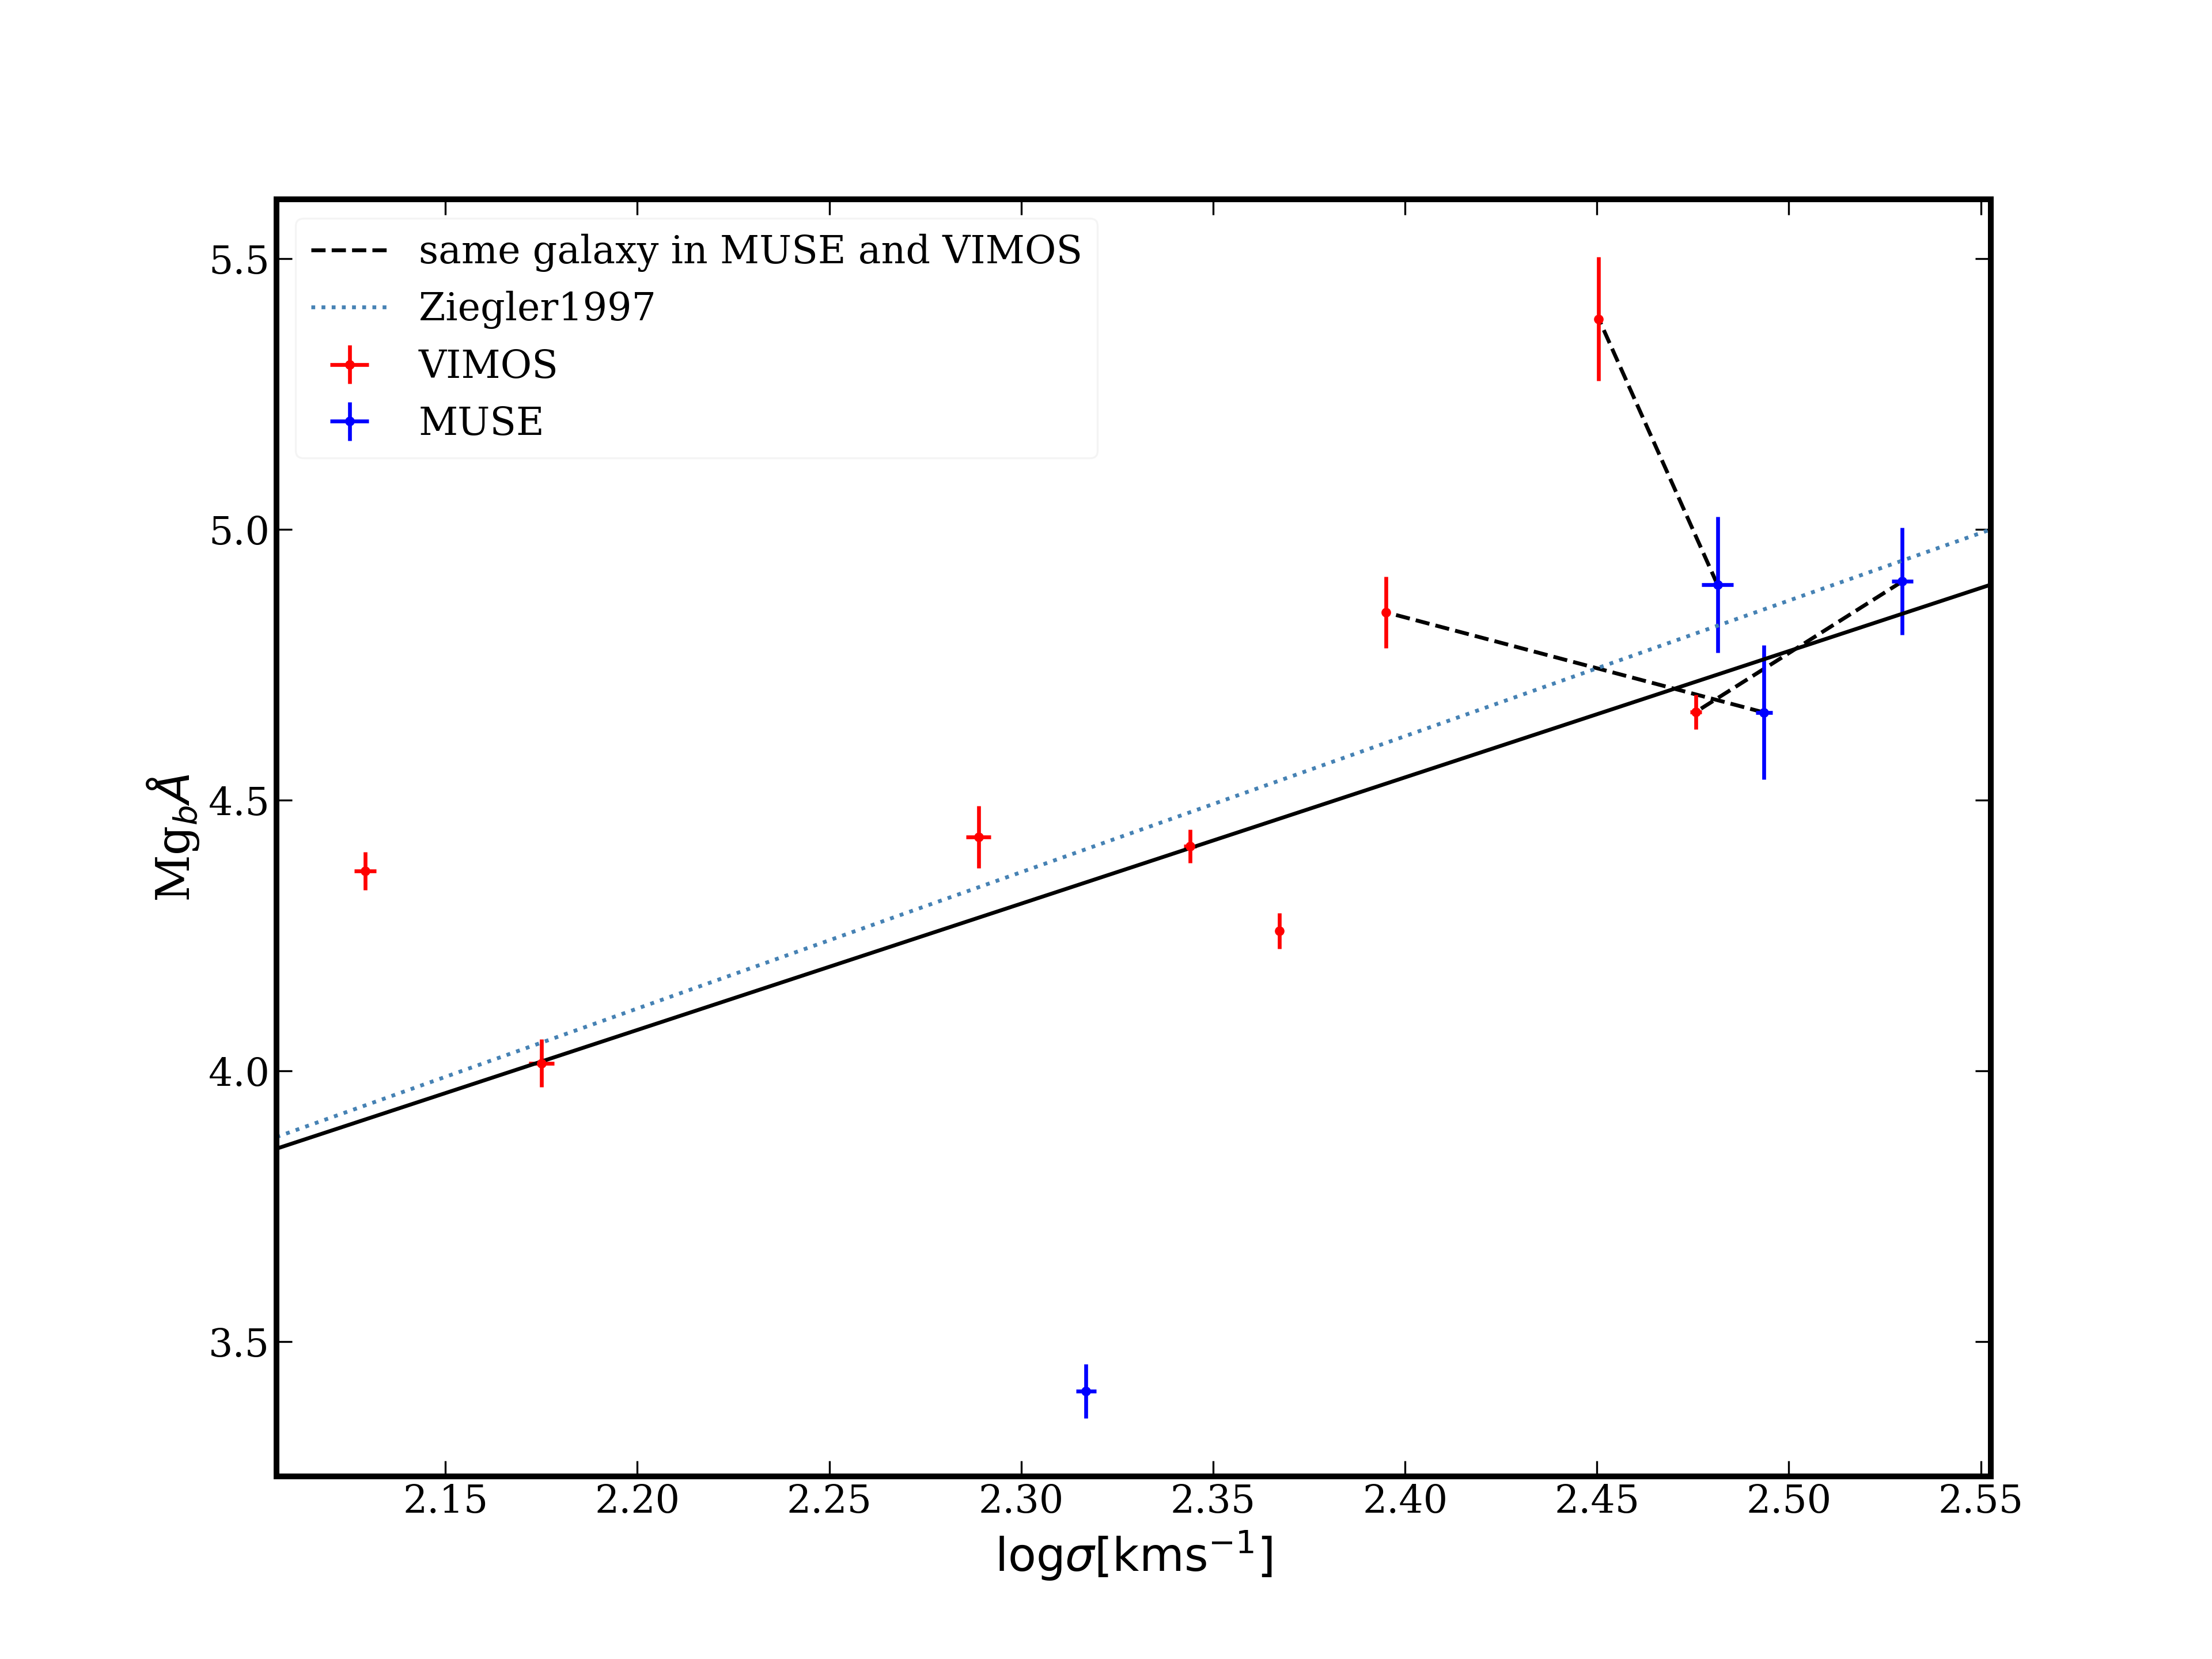
\includegraphics[width=.8\textwidth]{chapter4/Mg_sigma.png}
				\caption[Global Mg\,b--$\sigma$]{The Mg\,b -- velocity dispersion relation using a 2" aperture. We find a similar gradient to our best-fitting line (solid) to that found by \citet{Ziegler1997} shown as the dashed lines, but with a significant offset.}
				\label{fig:globalMg}
			\end{figure}

			\citet{Mehlert2003} shows the existence of the internal Mg--$\mathrm{\sigma}$ relation, but also suggests that it has a different origin to that of the global relation. They found that alpha-enhancement correlates with velocity dispersion and drives about 30\% of the global Mg--$\sigma$ relation. Metallicity variations provide the remaining 70\%. Alpha-enhancement usually has no radial gradient (while velocity dispersion is highly dependent on radius) suggesting that alpha-enhancement has no role in the internal Mg--$\sigma$ relation and it is entirely due to the metallicity radial gradient. We have therefore not shown internal Mg -- $\sigma$ relationships. Instead we investigate the radial gradient of the most-likely simple stellar populations (SSPs) in Section \ref{subsubsec:popGrad}.


		\subsubsection{Comparison to the Literature}
			\label{subsubsec:Lit}

			A comparison to the literature is difficult because of the inhomogeneous corrections applied by different authors. There are no standardized methods for accounting for emission lines from the ISM and/or stellar velocity dispersion. For example, some authors only correct for H\,$\beta$ emission, despite [\ion{O}{iii}] often being the strongest emission line in ETGs. This will effect the reliability of of Fe5015 index, since the [\ion{O}{iii}] doublet falls within its bandpasses. [\ion{N}{i}] emission will affect the Mg\,b index in the same way. 

			Some indices are extremely sensitive to the stellar velocity dispersion correction. For example, due to the steepness of the pseudo-continuum in the G4300 index, a change of $30 \, \mathrm{km\,s^{-1}}$ can affect the corrected index value by as much as 2\,\AA.

			When comparing to a particular paper we correct for the same effects as described in the paper, but using our methods as described in Section \ref{subsubsec:Absorption}. We use a resolution of 8.4\,\AA\ (FWHM) in order to use the transformation function provided by \citet{Vazdekis2010} to convert from Lick calibrated measurements to the Line Index System (LIS; see Section \ref{subsubsec:Absorption}). 

			Table \ref{tab:litAbsorption} summarises our comparisons to the literature. For the comparison to \citet{Vazdekis2010}, we analysed the SAURON dataset\footnote{http://www.strw.leidenuniv.nl/sauron/} \citep{Emsellem2004} using the same pipeline as for our sample. 


% Should SARUON comparison be in Chapter 2 as a test of the pipeline?
			\begin{table}
				\centering
			\begin{threeparttable}
				\caption{Comparisons of measured absorption line indices to the literature.}
				\label{tab:litAbsorption}
				\begin{tabular*}{0.8\textwidth}{@{\extracolsep{\fill}}l r r r}
					\hline
					\hline
					Index 		& \multicolumn{1}{c}{N$_\mathrm{gals}$} & \multicolumn{1}{c}{Offset} & \multicolumn{1}{c}{Dispersion} \\
								& 		&\multicolumn{1}{c}{\AA}& \multicolumn{1}{c}{\AA} \\
					\hline
					\multicolumn{4}{c}{\citet{Vazdekis2010} (SAURON)} \\
					\hline
					H\,$\beta$ 	& 46		& -0.02\leavevmode\phantom{0}& 0.25\leavevmode\phantom{0}	\\
					Fe5015		& 46		& 0.66\leavevmode\phantom{0}& 0.34\leavevmode\phantom{0}	\\
					Mg\,b 		& 46		& 0.06\leavevmode\phantom{0}& 0.33\leavevmode\phantom{0}	\\
					\hline
					\multicolumn{4}{c}{\citet{Rampazzo2005} (VIMOS)} \\
					\hline
					G4300 		& 3 		& 2.29\leavevmode\phantom{0}& 0.11\leavevmode\phantom{0}	\\
					Fe4383 		& 3 		& 0.39\leavevmode\phantom{0}& 0.23\leavevmode\phantom{0}	\\
					Ca4455 		& 3 		& -0.19\leavevmode\phantom{0}& 0.09\leavevmode\phantom{0}	\\
					Fe4531 		& 3 		& 0.16\leavevmode\phantom{0}& 0.26\leavevmode\phantom{0}	\\
					H\,$\beta$ 	& 3 		& 0.17\leavevmode\phantom{0}& 0.12\leavevmode\phantom{0}	\\
					Fe5015 		& 3 		& -0.73\leavevmode\phantom{0}& 0.48\leavevmode\phantom{0}	\\
					Mg\,b 		& 3 		& -0.43\leavevmode\phantom{0}& 0.17\leavevmode\phantom{0}	\\
					\hline
					\multicolumn{4}{c}{\citet{Rampazzo2005} (MUSE)} \\
					\hline
					H\,$\beta$ 	& 2 		& -0.28\leavevmode\phantom{0}& 0.17\leavevmode\phantom{0}	\\ 
					Fe5015 		& 2 		& 0.87\leavevmode\phantom{0}& 0.34\leavevmode\phantom{0}	\\ 
					Mg\,b 		& 2 		& 0.31\leavevmode\phantom{0}& 0.14\leavevmode\phantom{0}	\\
					Fe5270 		& 2 		& -0.11\leavevmode\phantom{0}& 0.15\leavevmode\phantom{0}	\\
					Fe5335 		& 2 		& 0.08\leavevmode\phantom{0}& 0.15\leavevmode\phantom{0}	\\
					Fe5406 		& 2 		& 0.16\leavevmode\phantom{0}& 0.07\leavevmode\phantom{0}	\\
					Fe5709 		& 2 		& 0.11\leavevmode\phantom{0}& 0.10\leavevmode\phantom{0}	\\
					Fe5782 		& 2 		& -0.03\leavevmode\phantom{0}& 0.11\leavevmode\phantom{0}	\\
					NaD 		& 2 		& 0.90\leavevmode\phantom{0}& 0.41\leavevmode\phantom{0}	\\
					TiO1 (mag)	& 2 		& -0.004	& 0.003	\\
					TiO2 (mag)	& 2 		& -0.011	& 0.007	\\
					\hline
					\multicolumn{4}{c}{\citet{Ogando2008} (VIMOS)} \\
					\hline
					H\,$\beta$ 	& 6 		& 0.07\leavevmode\phantom{0}& 0.60\leavevmode\phantom{0}	\\
					Fe5015 		& 6 		& -0.09\leavevmode\phantom{0}& 0.15\leavevmode\phantom{0}	\\
					Mg\,b 		& 6 		& -0.70\leavevmode\phantom{0}& 0.08\leavevmode\phantom{0}	\\
					\hline
					\multicolumn{4}{c}{\citet{Ogando2008} (MUSE)} \\
					\hline
					H\,$\beta$ 	& 3 		& -0.04\leavevmode\phantom{0}& 0.23\leavevmode\phantom{0}	\\ 
					Fe5015 		& 3 		& -0.16\leavevmode\phantom{0}& 0.33\leavevmode\phantom{0}	\\ 
					Mg\,b 		& 3 		& -1.10\leavevmode\phantom{0}& 0.26\leavevmode\phantom{0}	\\
					Fe5270 		& 3 		& -0.66\leavevmode\phantom{0}& 0.16\leavevmode\phantom{0}	\\
					Fe5335 		& 3 		& -0.66\leavevmode\phantom{0}& 0.11\leavevmode\phantom{0}	\\
					Fe5406 		& 3 		& -0.51\leavevmode\phantom{0}& 0.06\leavevmode\phantom{0}	\\
					Fe5709 		& 3 		& -0.22\leavevmode\phantom{0}& 0.08\leavevmode\phantom{0}	\\
					NaD 		& 3 		& -1.57\leavevmode\phantom{0}& 0.16\leavevmode\phantom{0}	\\
					\hline
					\hline
				\end{tabular*}
				\begin{tablenotes}
				\footnotesize
				\note Comparisons to \citet{Rampazzo2005} are sampled at 7 radial apertures for each galaxy: 1.5, 2.5 and 10.0 arcsec and R$_e$/10, R$_e$/8, R$_e$/4 and R$_e$/2. 
				\item Col.\,1: Index; Col.\,2: Number of galaxies in comparison; Col.\,3: Offset = mean(lit value - our value); Col.\,4: Dispersion = standard deviation (lit value - our value).
				\end{tablenotes}
			\end{threeparttable}
			\end{table}

			We note that G4300 has a very large offset with respect to the results of \citet{Rampazzo2005}. As noted above, this index is extremely sensitive to the stellar velocity dispersion correction. We measure the stellar velocity dispersion to be different to that found by \citet{Rampazzo2005} by an average of $21\,\mathrm{km\,s^{-1}}$. 

% How do these compare? Is this good or not




	\subsection{Most-likely stellar population model}
		\label{subsec:ssp}
		We have assumed that each bin in each galaxy from our Southern sample can be well described by a SSP. We use the method described in section \ref{subsubsec:StellarPop} to find maps of the most-likely SSP characteristics: age (t), metallicity (Z/H) and alpha enhancement ($\mathrm{\alpha/Fe}$) from the absorption line strength maps. 

		Figs.\,\ref{fig:VIMOS_pop} and \ref{fig:MUSE_pop} show the resolved most-likely stellar populations for our Southern sample. In general they show old, metal rich and alpha enhanced SSPs; qualities which ETGs are well known for. The exceptions are NGC 612 and NGC 1316. NGC 612 is discussed in more detail in section \ref{sec:NGC612}, while NGC 1316 shows a very young stellar population (our fit agrees with that of \citealt{Kuntschner2000}, but is conflicting with the older and less metal rich stellar population found by \citealt{Koleva2011} who found $t=4.5 \pm 0.3 \,\mathrm{Gyr}$ and $[Fe/H]=0.12 \pm 0.01 \,\mathrm{[Fe/H]_\odot}$ for an aperture covering the central 0.1 kpc). 

		\begin{figure}
			\centering
			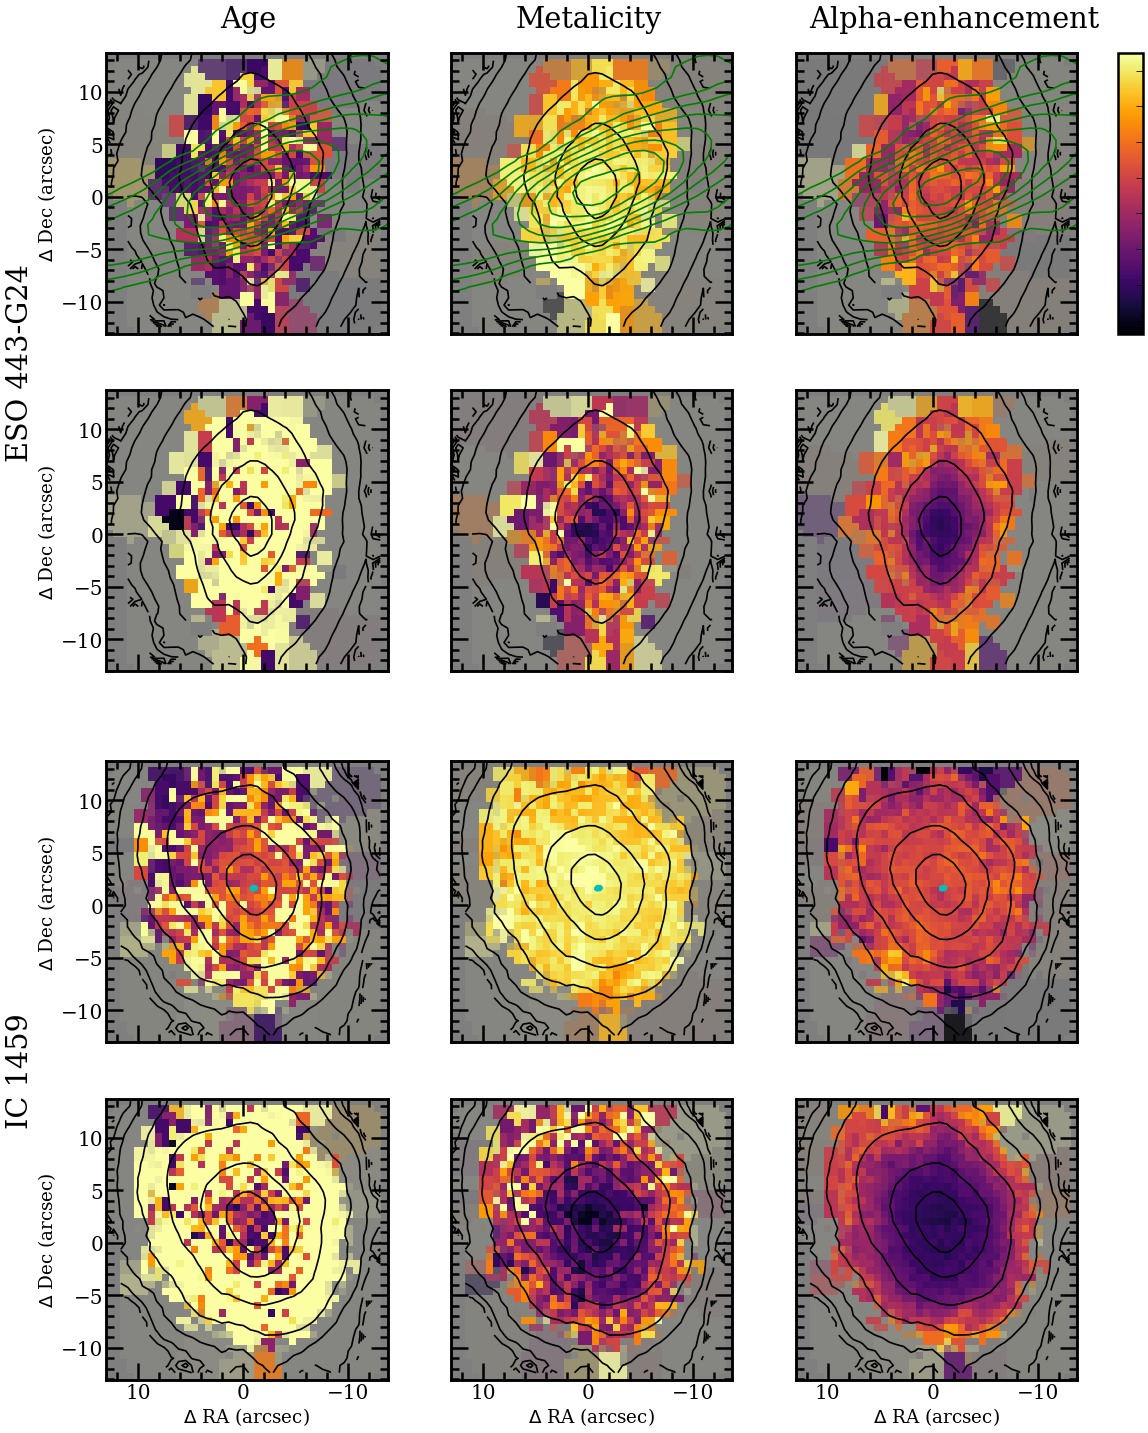
\includegraphics[height=0.94\textheight]{chapter4/vimos/pop1.png}
			\caption[VIMOS stellar population maps]{VIMOS stellar population maps: Left to right: age, metallicity and alpha enhancement; Top to bottom: ESO 443-G24, IC 1459 and IC 1531. Alternate rows show a given parameter its associated uncertainty. Contours are as in Fig.\,\ref{fig:VIMOS_stellar}. The colour scales have limits of 0--15\,Gyr, -2.25--0.67\,$\mathrm{[Fe/H]_\odot}$ and -0.3--0.5\,$\mathrm{[\alpha/FeH]_\odot}$ for age, metallicity and alpha-enhancement maps and 0--2\,Gyr, 0--0.4\,$\mathrm{[Fe/H]_\odot}$ and 0--0.25\,$\mathrm{[\alpha/Fe]_\odot}$ for their respective associated uncertainties.}
			\label{fig:VIMOS_pop}
		\end{figure}
		\begin{figure}
			\centering
			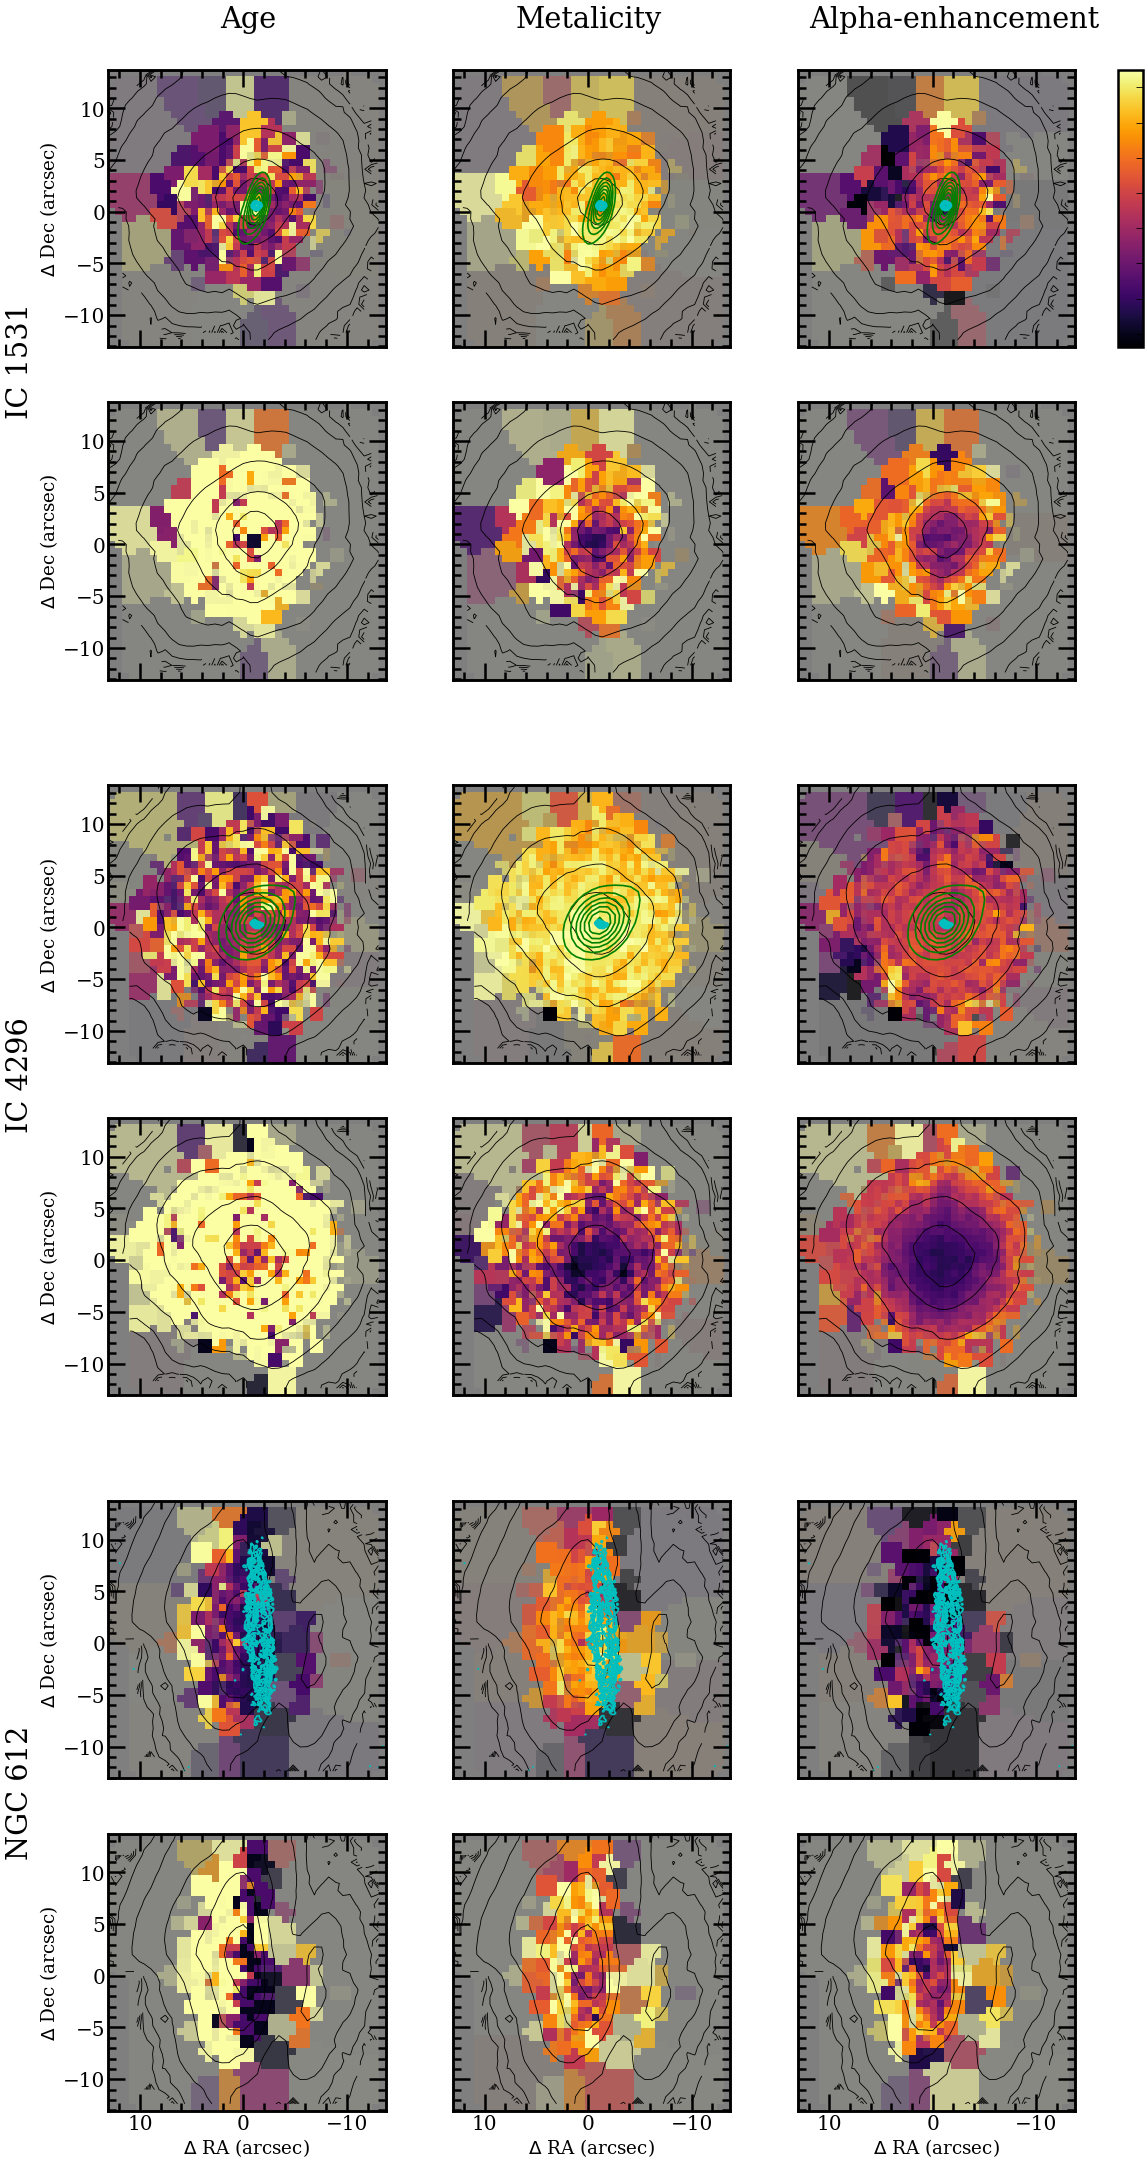
\includegraphics[height=0.94\textheight]{chapter4/vimos/pop2.png}
			\contcaption{\textit{Continued.}}% for IC 4296, NGC 612 and NGC 1399}
		\end{figure}
		\begin{figure}
			\centering
			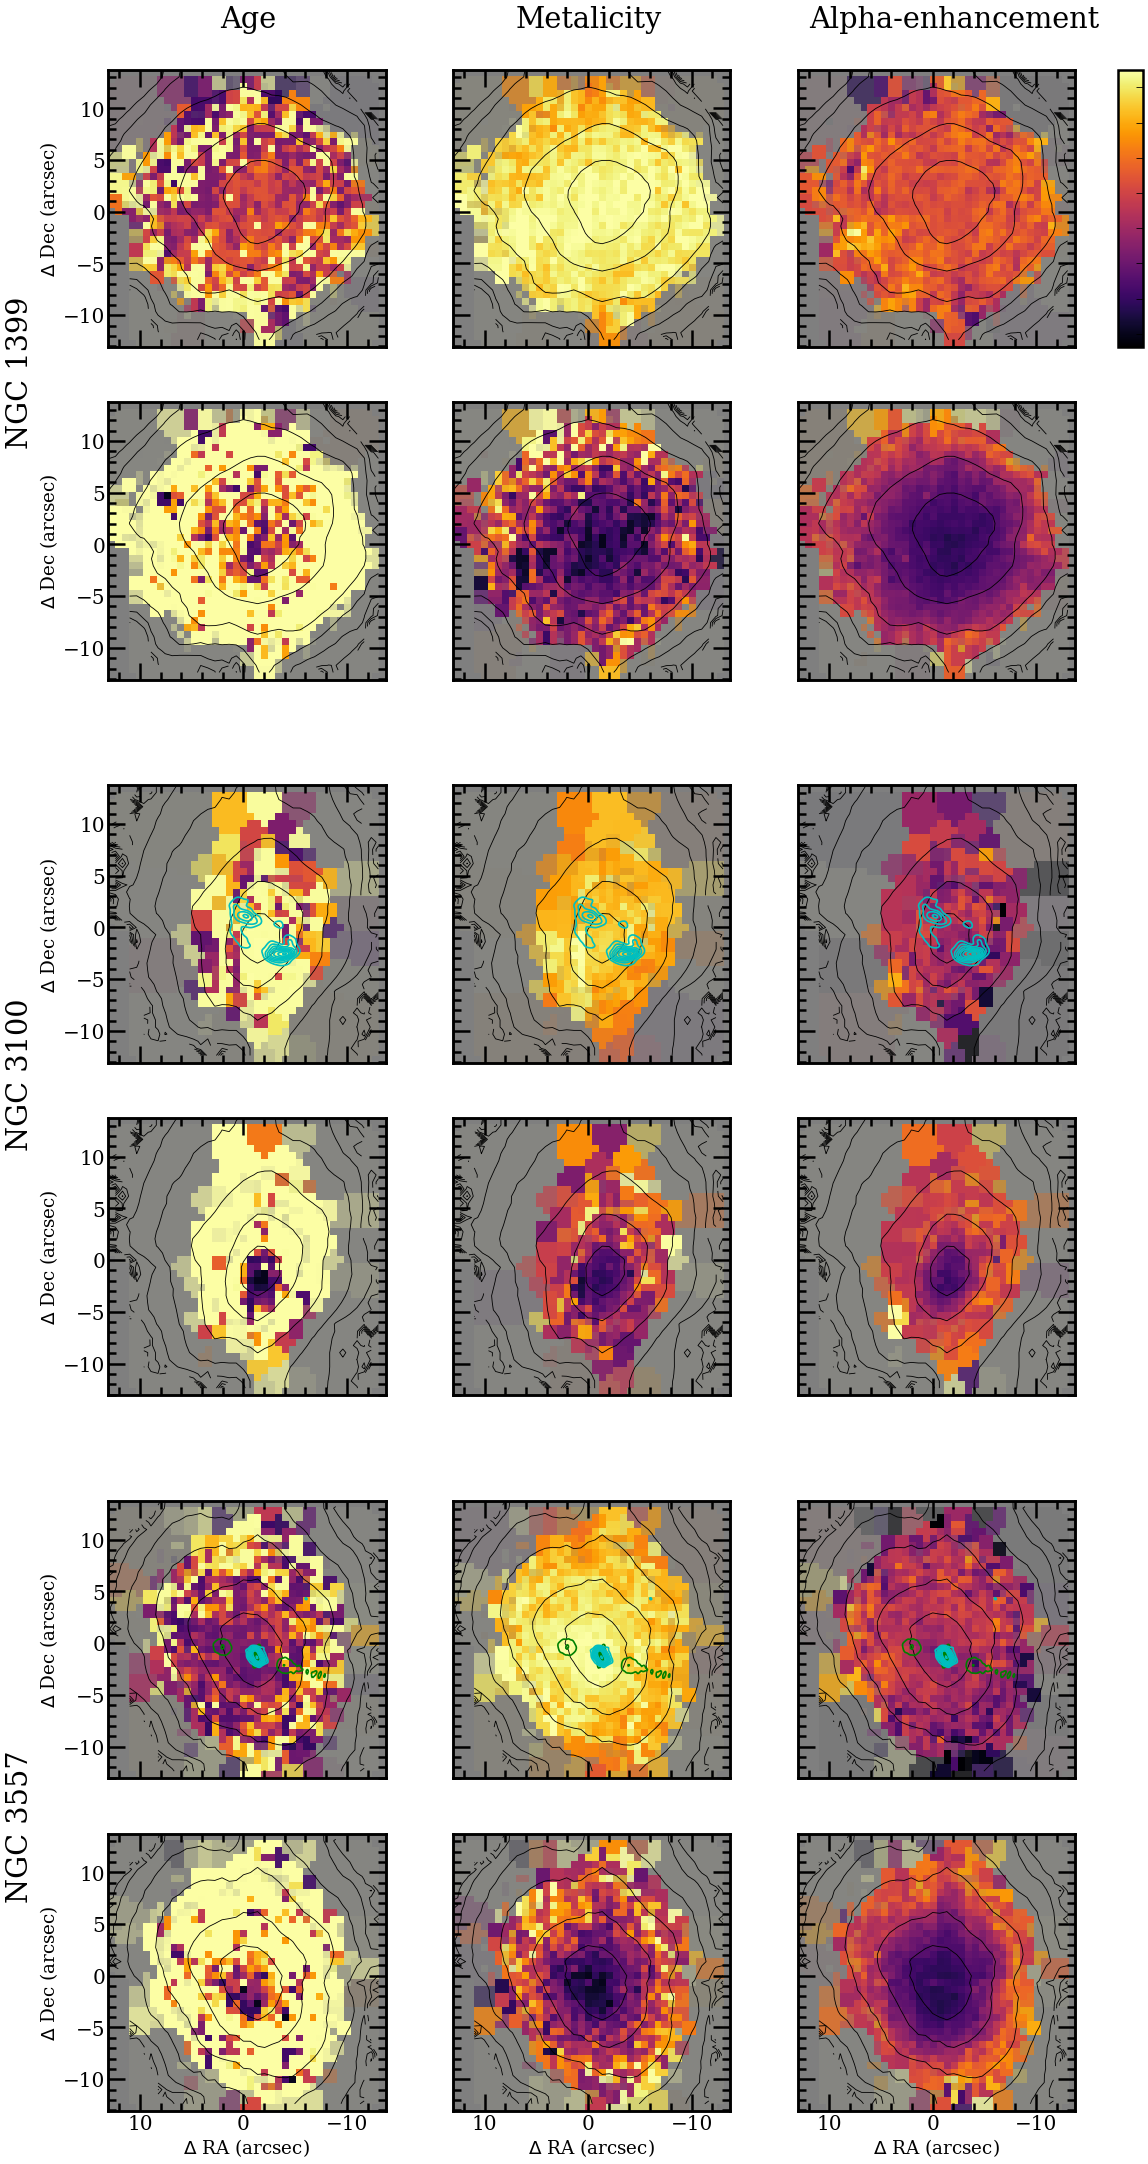
\includegraphics[height=0.94\textheight]{chapter4/vimos/pop3.png}
			\contcaption{\textit{Continued.}}% for NGC 3100, NGC 3557 and NGC 7075}
		\end{figure}
		\begin{figure}
			\centering
			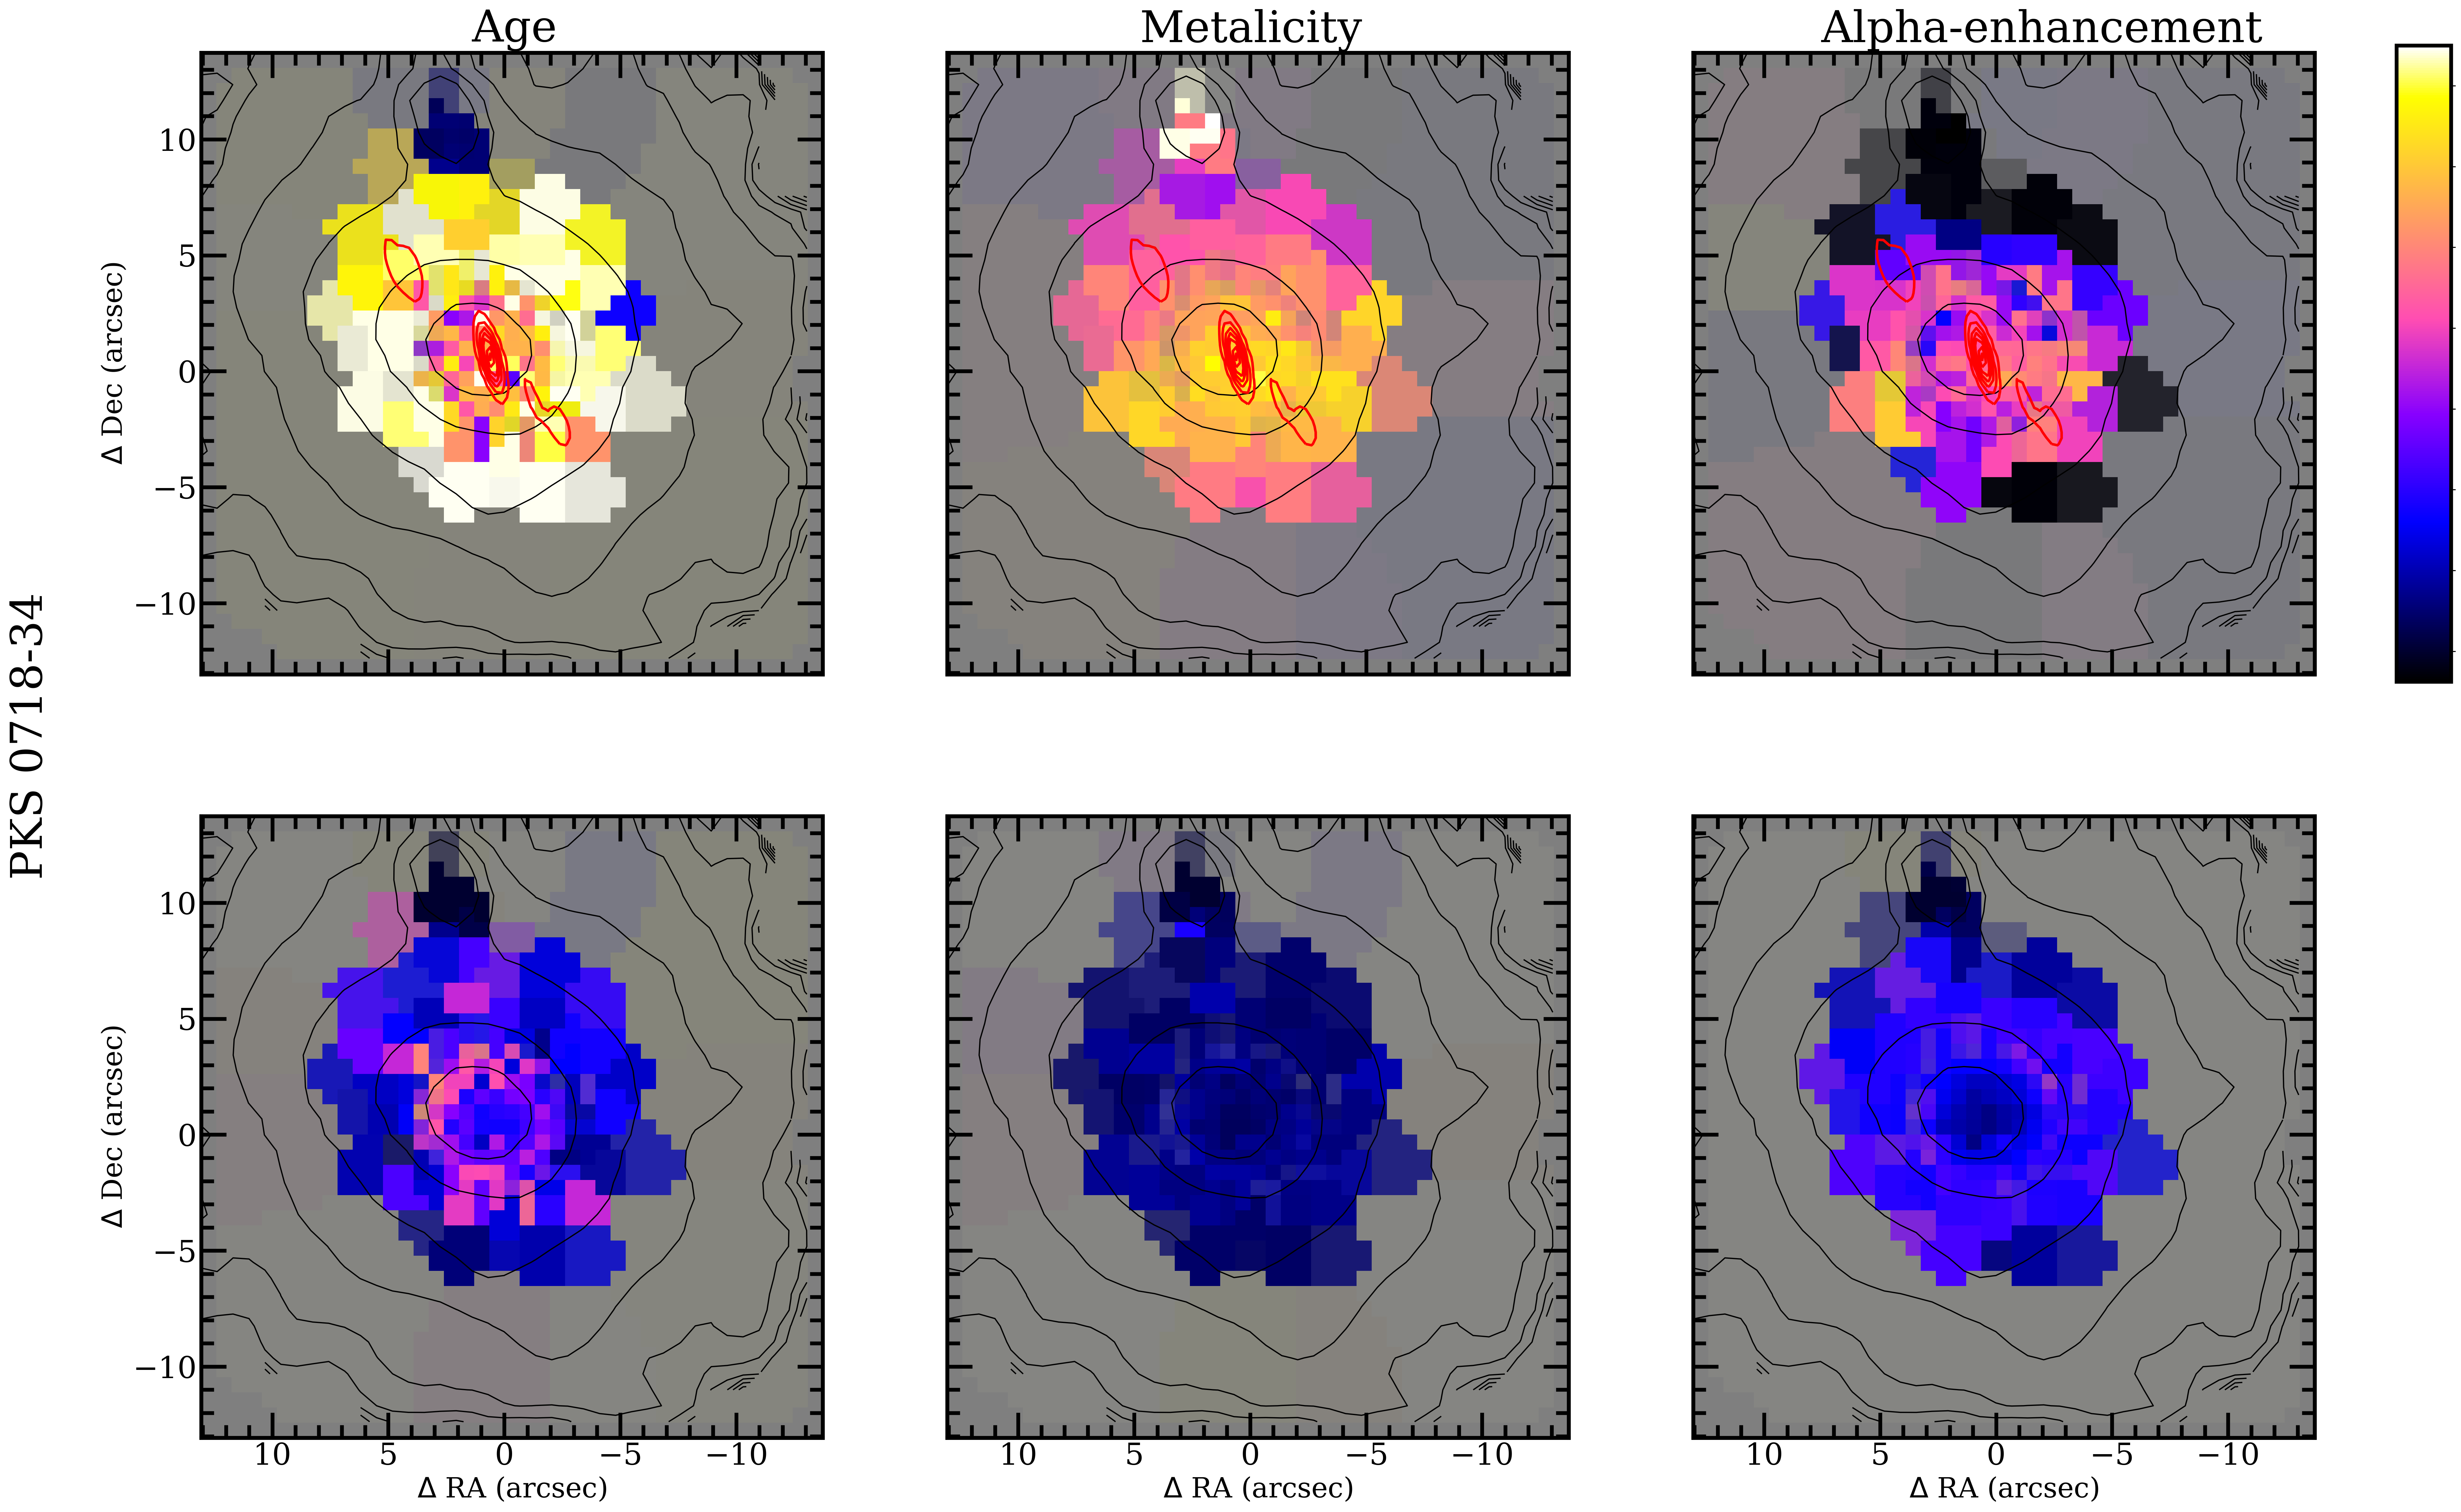
\includegraphics[height=0.31\textheight]{chapter4/vimos/pop4.png}
			\contcaption{\textit{Continued.}}% for PKS 718-34}
		\end{figure}

		\begin{figure}
			\centering
			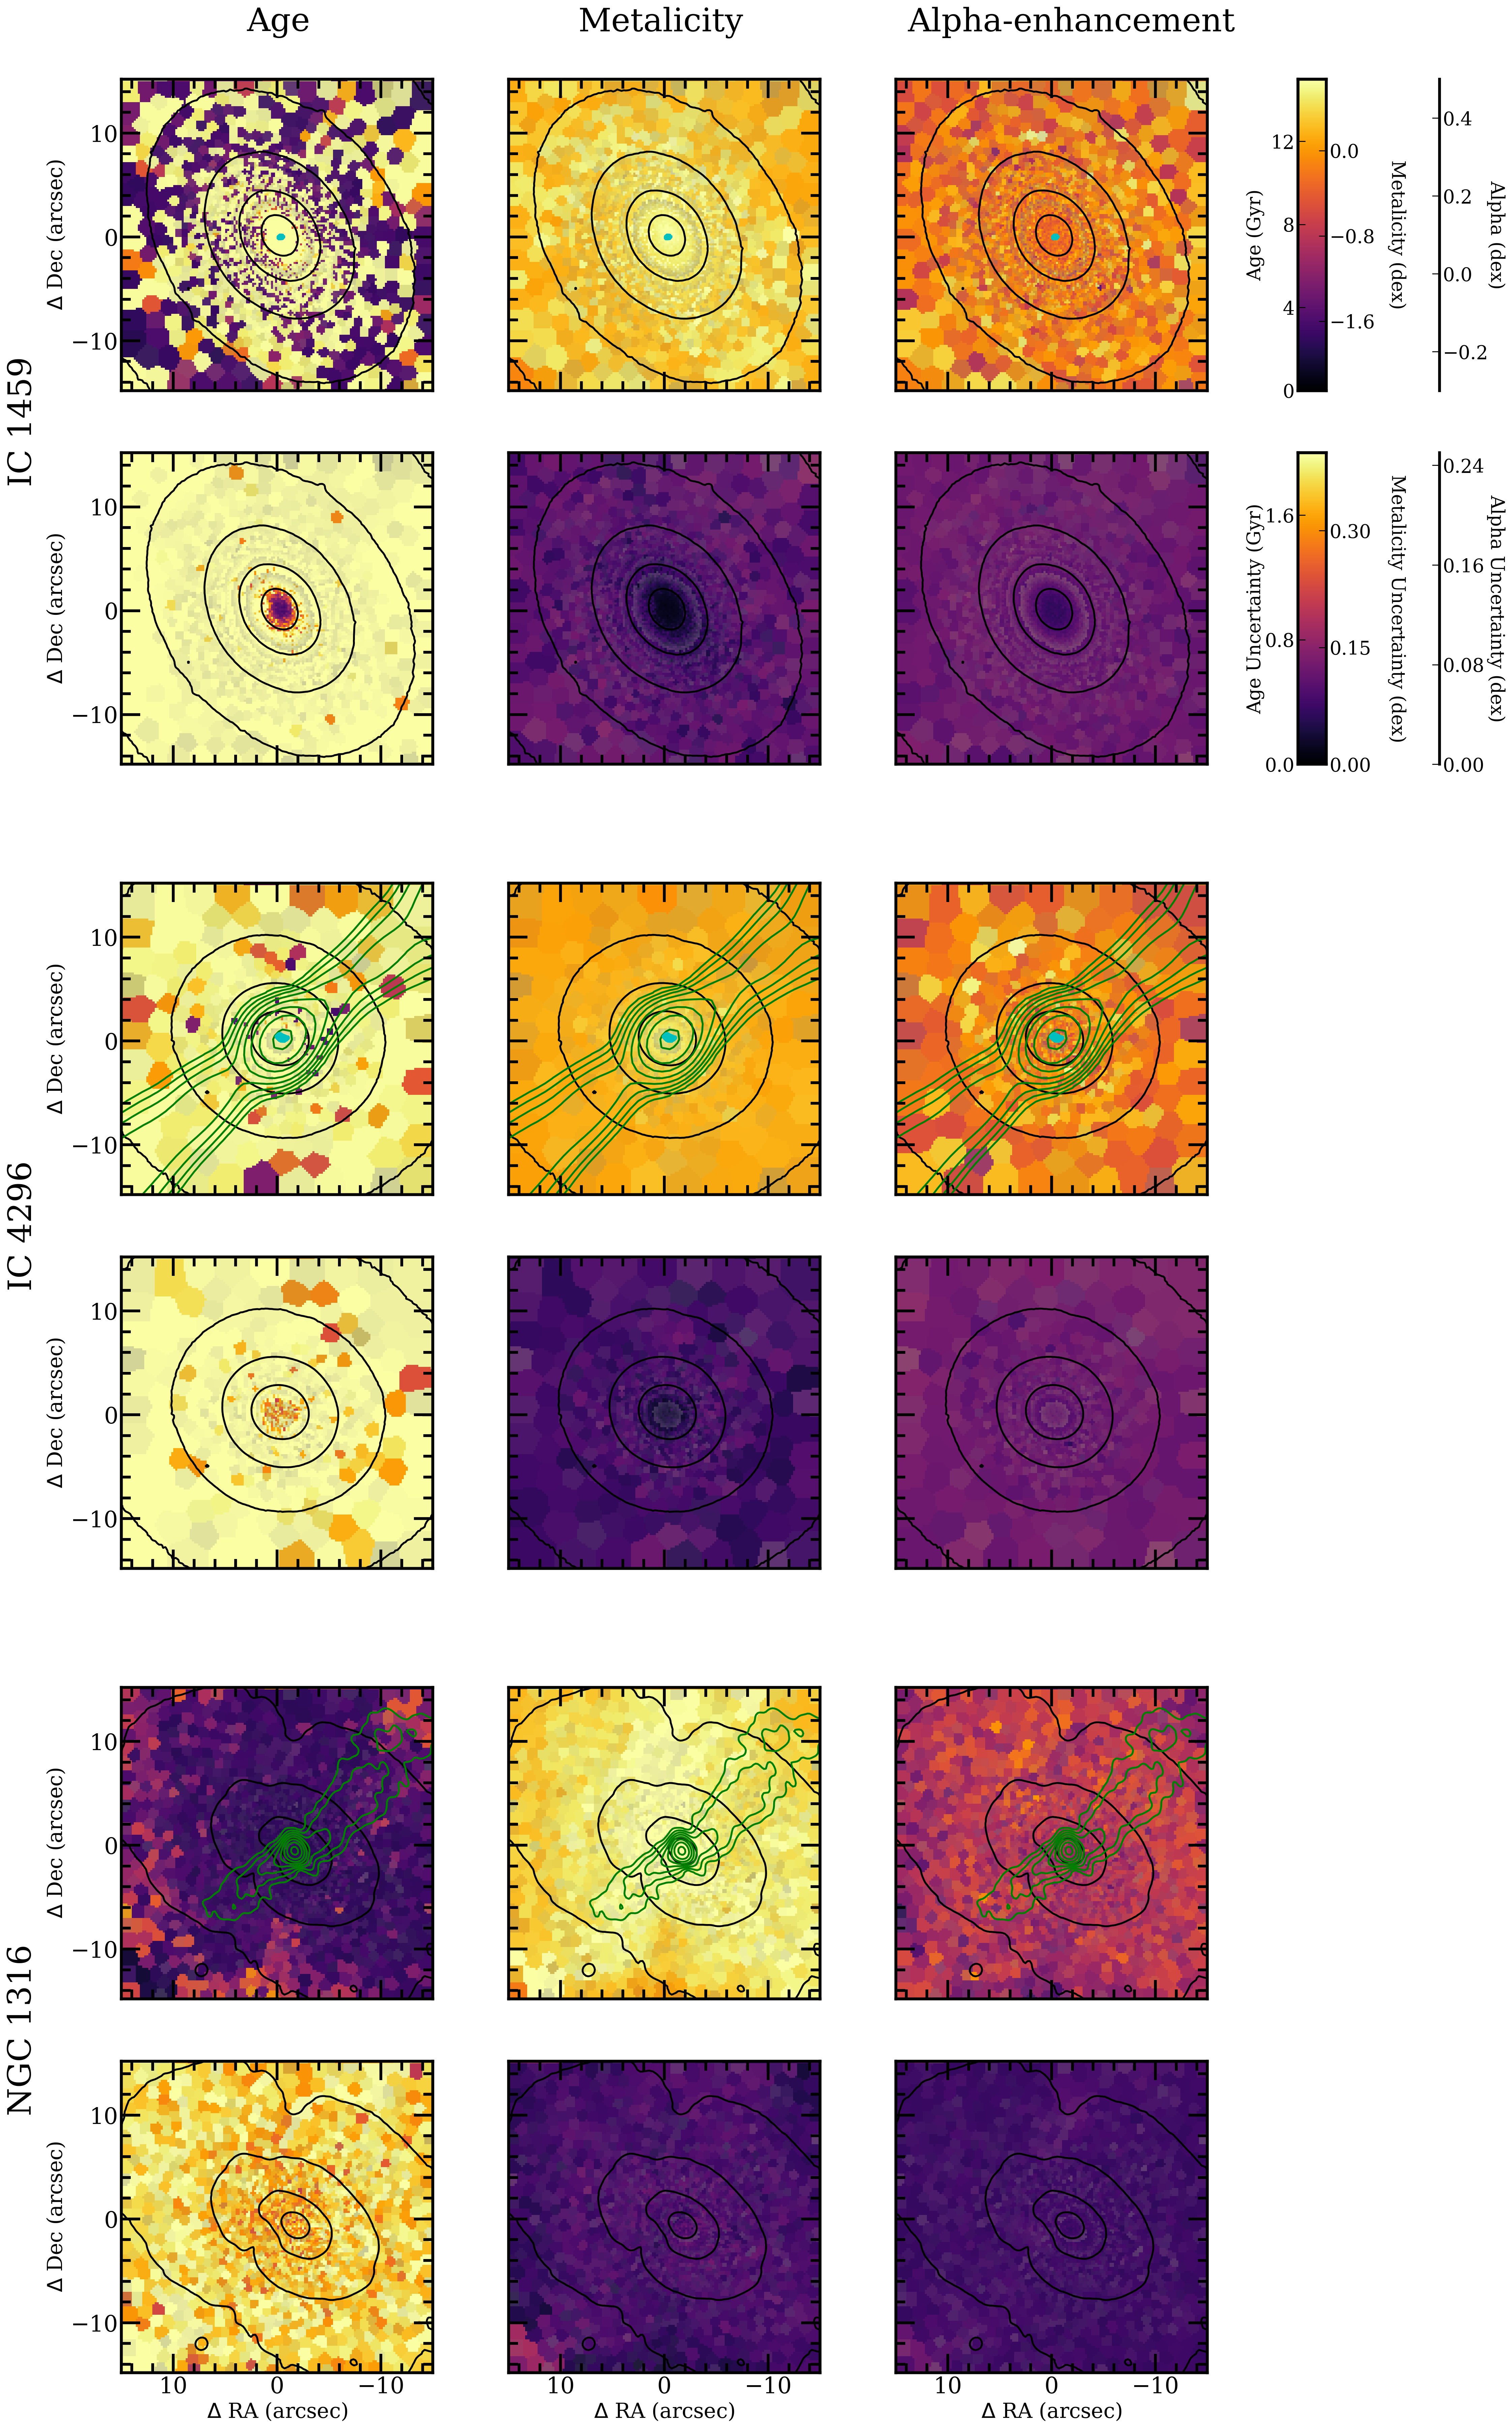
\includegraphics[height=0.94\textheight]{chapter4/muse/pop1.png}
			\caption[MUSE stellar population maps]{As in Figure \ref{fig:VIMOS_pop} but for the MUSE stellar population maps.}
			\label{fig:MUSE_pop}
		\end{figure}
		\begin{figure}
			\centering
			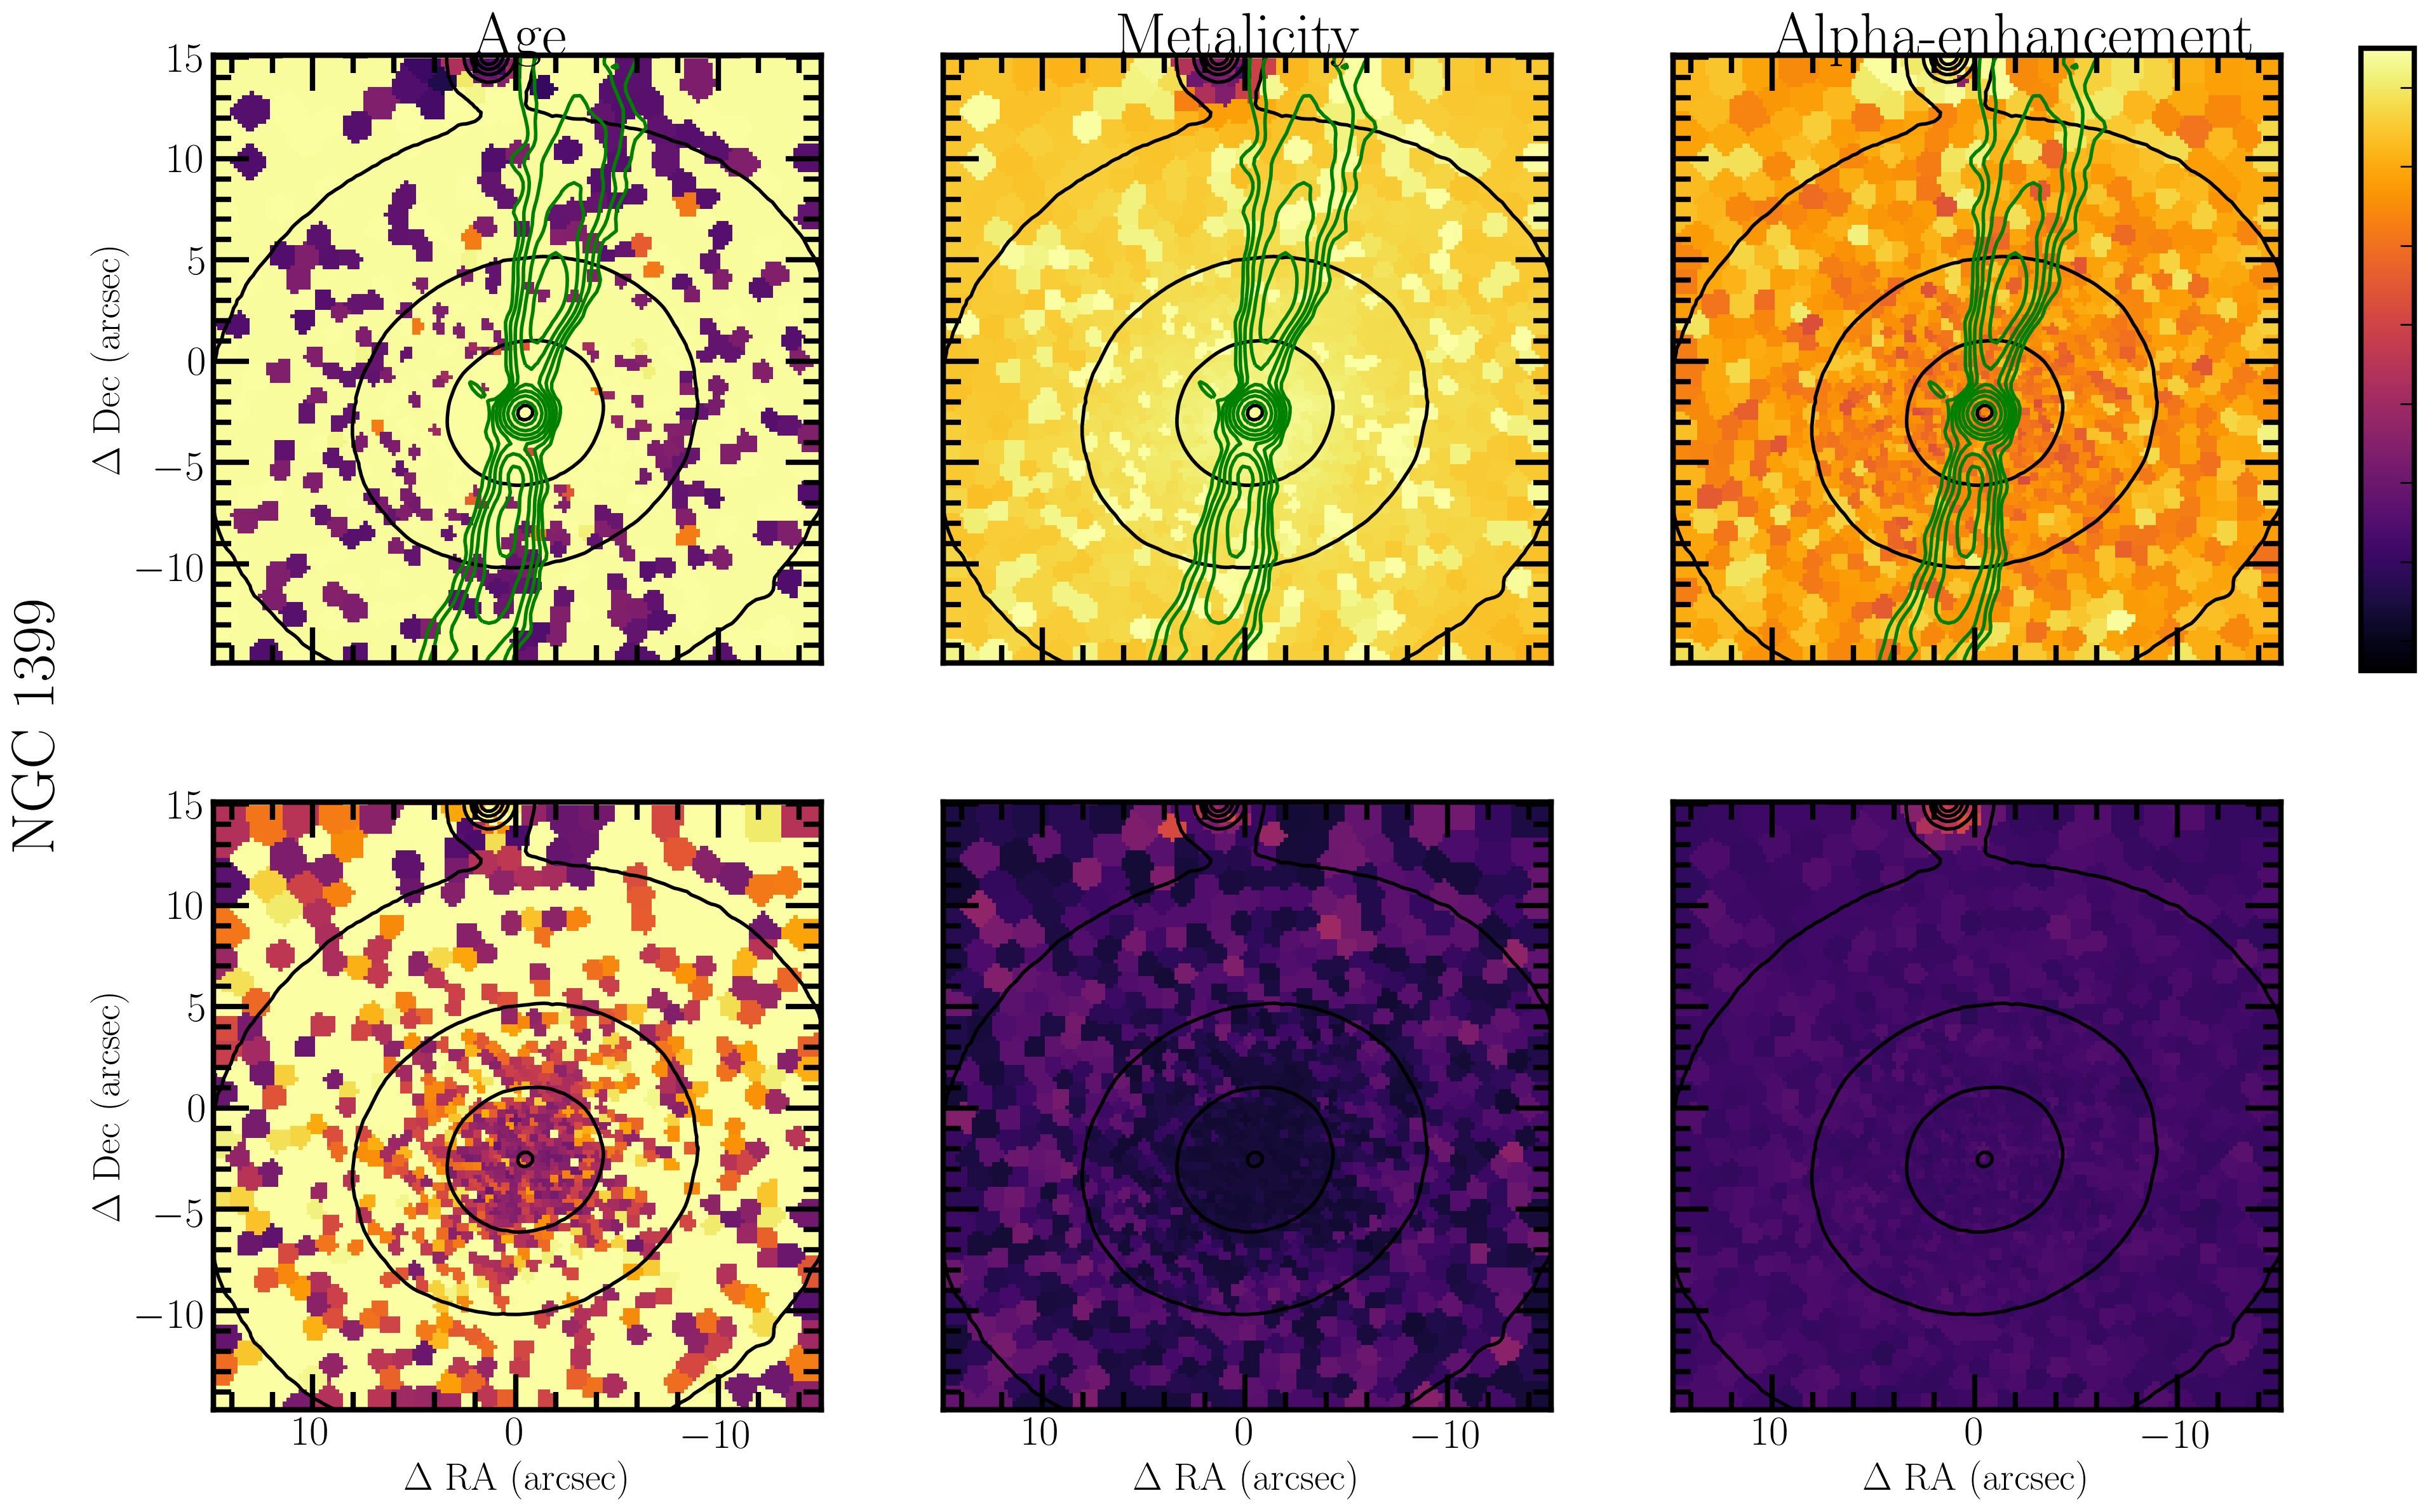
\includegraphics[height=0.31\textheight]{chapter4/muse/pop2.png}
			\contcaption{\textit{Continued.}}
		\end{figure}

		If molecular (cold) gas is the fuel source that is accreted on to the the central black holes of our Southern sample in order to power the radio jets, unless it is accreted in a highly turbulent fashion, it might be expected that some of that gas might form stars \citep[e.g.][]{Collin1999, Diamond-Stanic2012, LaMassa2013}. If this is the case then a young stellar population might be expected to dominate in the very central (1--2) spaxels. We note that our maps show no evidence of this. 


		\subsubsection{Radial Gradients in Stellar Populations}
			\label{subsubsec:popGrad}

			\citet{Koleva2011} showed that while individual galaxies can have a wide range of radial gradients of age and metallicity, the mean gradient (within a mass bin) is uniform across a large mass range. They assume a linear relationship between $\log t$ or $[Fe/H]$ and $\log (R/\mathrm{R_e})$. The results from our southern sample are shown in table \ref{tab:popGrad}. 

			\begin{table}
				\centering
				\caption{The radial gradients of the most-likely SSP models.}
				\label{tab:popGrad}
				\begin{tabular}{l c c}
					\hline
					\hline 
					Galaxy 	& $\Delta_\text{log age}$ & $\Delta_\text{[Fe/H]}$ \\ 
						& log(Gyr) arcsec$^{-1}$ & [Fe/H]$_\odot$ arcsec$^{-1}$ \\
					\hline
					ESO 443-G024 & $-0.008 \pm 0.006$ & $-0.028 \pm 0.005$ \\
					IC 1459 	& $-0.024 \pm 0.011$ & $-0.024 \pm 0.022$ \\
					IC 1531 	& $-0.016 \pm 0.006$ & $0.004 \pm 0.009$ \\
					IC 4296		& $0.001 \pm 0.001$ & $0.071 \pm 0.006$ \\
					NGC 612 	& $0.021 \pm 0.024$ & $-0.101 \pm 0.012$ \\
					NGC 1316 	& $0.007 \pm 0.004$ & $0.005 \pm 0.006$ \\
					NGC 1399 	& $-0.035 \pm 0.008$ & $0.041 \pm 0.006$ \\
					NGC 3100 	& $0.000 \pm 0.004$ & $-0.045 \pm 0.003$ \\
					NGC 3557 	& $0.000 \pm 0.006$ & $-0.023 \pm 0.007$ \\
					NGC 7075 	& $0.006 \pm 0.003$ & $-0.067 \pm 0.006$ \\
					PKS 718-34  & $0.008 \pm 0.007$ & $-0.115 \pm 0.007$ \\
					\hline
					\hline
				\end{tabular}
			\end{table}

			We find average gradients of $\Delta_\text{log age} = -0.004\pm0.003 \,\mathrm{log(Gyr) \, arcsec^{-1}}$ and $\Delta_\text{[Fe/H]} = -0.025\pm0.002 \mathrm{[Fe/H]_\odot \, arcsec^{-1}}$. This is consistent with \citet{Koleva2011} who, for elliptical galaxies found average gradients of $0.06\pm0.09 \, \mathrm{log(Gyr) \, arcsec^{-1}}$ and $-0.26\pm0.08 \, \mathrm{[Fe/H]_\odot \, arcsec^{-1}}$ for the age and metallicity gradients, respectively. For S0s they find flatter corresponding gradients of $0.01\pm0.11\, \mathrm{log(Gyr) \, arcsec^{-1}}$ and $-012\pm0.13\, \mathrm{[Fe/H]_\odot \, arcsec^{-1}}$. 

% SSP -- sigma relation here?



	\subsection{Kinematically-Decoupled Cores}
		\label{subsec:popKDC}

		\citet{Kuntschner2010} found that kinematically-decoupled cores (KDCs) exist in two classes: they are either small or contain an old stellar population. The size of the KDC is defined as the radius of the region surrounding the KDC where the superposition of the two components (the KDC and the host galaxy) results in a local minimum in the mean velocity. The KDC age is defined as the age of the most-likely SSP model for the spatially integrated spectrum within an aperture 1 arcsec on the centre of the galaxy.

		The small KDCs tend to be found in fast rotators with young global stellar populations and have still younger stellar populations within the KDC. They also tend to be counter-rotating or very close to counter-rotating with respect to the host galaxy. \citet{Kuntschner2010} suggests that the dominance of the stellar light of these KDCs over the other stars in the centre of the galaxies will reduce as time passes. As such, it is thought that old, small KDCs do exist, but they are not observable. \citet{Kuntschner2010} go on to propose that these KDCs are the result of gas accreted into the galaxy, settling into a counter-rotating disc near the centre of the galaxy, before forming the stars that make up the KDC. 

		The large KDCs are typically embedded in slow rotators. They have no limit on the age of their stellar populations suggesting that the stars within the KDC dominate in total mass as well as surface brightness. Thus, they do not fade into their host galaxies as they age unlike the small KDCs. \citet{Bois2011} showed major mergers may well result in such large KDCs if the initial spin axis of the progenitor galaxy with the lowest bulge-to-disk ratio (later-type) is anti-parallel to the orbital angular momentum vector. 

		In Fig.\,\ref{fig:KDC} we show the age and size of the 3 KDCs hosted by galaxies in our Southern sample. We include PKS 718-34 here but stress it is only tentatively classified as containing a KDC. As can be seen from Fig.\,\ref{fig:KDC} while PKS 718-34 would be an extremely large KDC it still is consistent with the findings of \citet{Kuntschner2010}.

		\begin{figure}
			\centering
			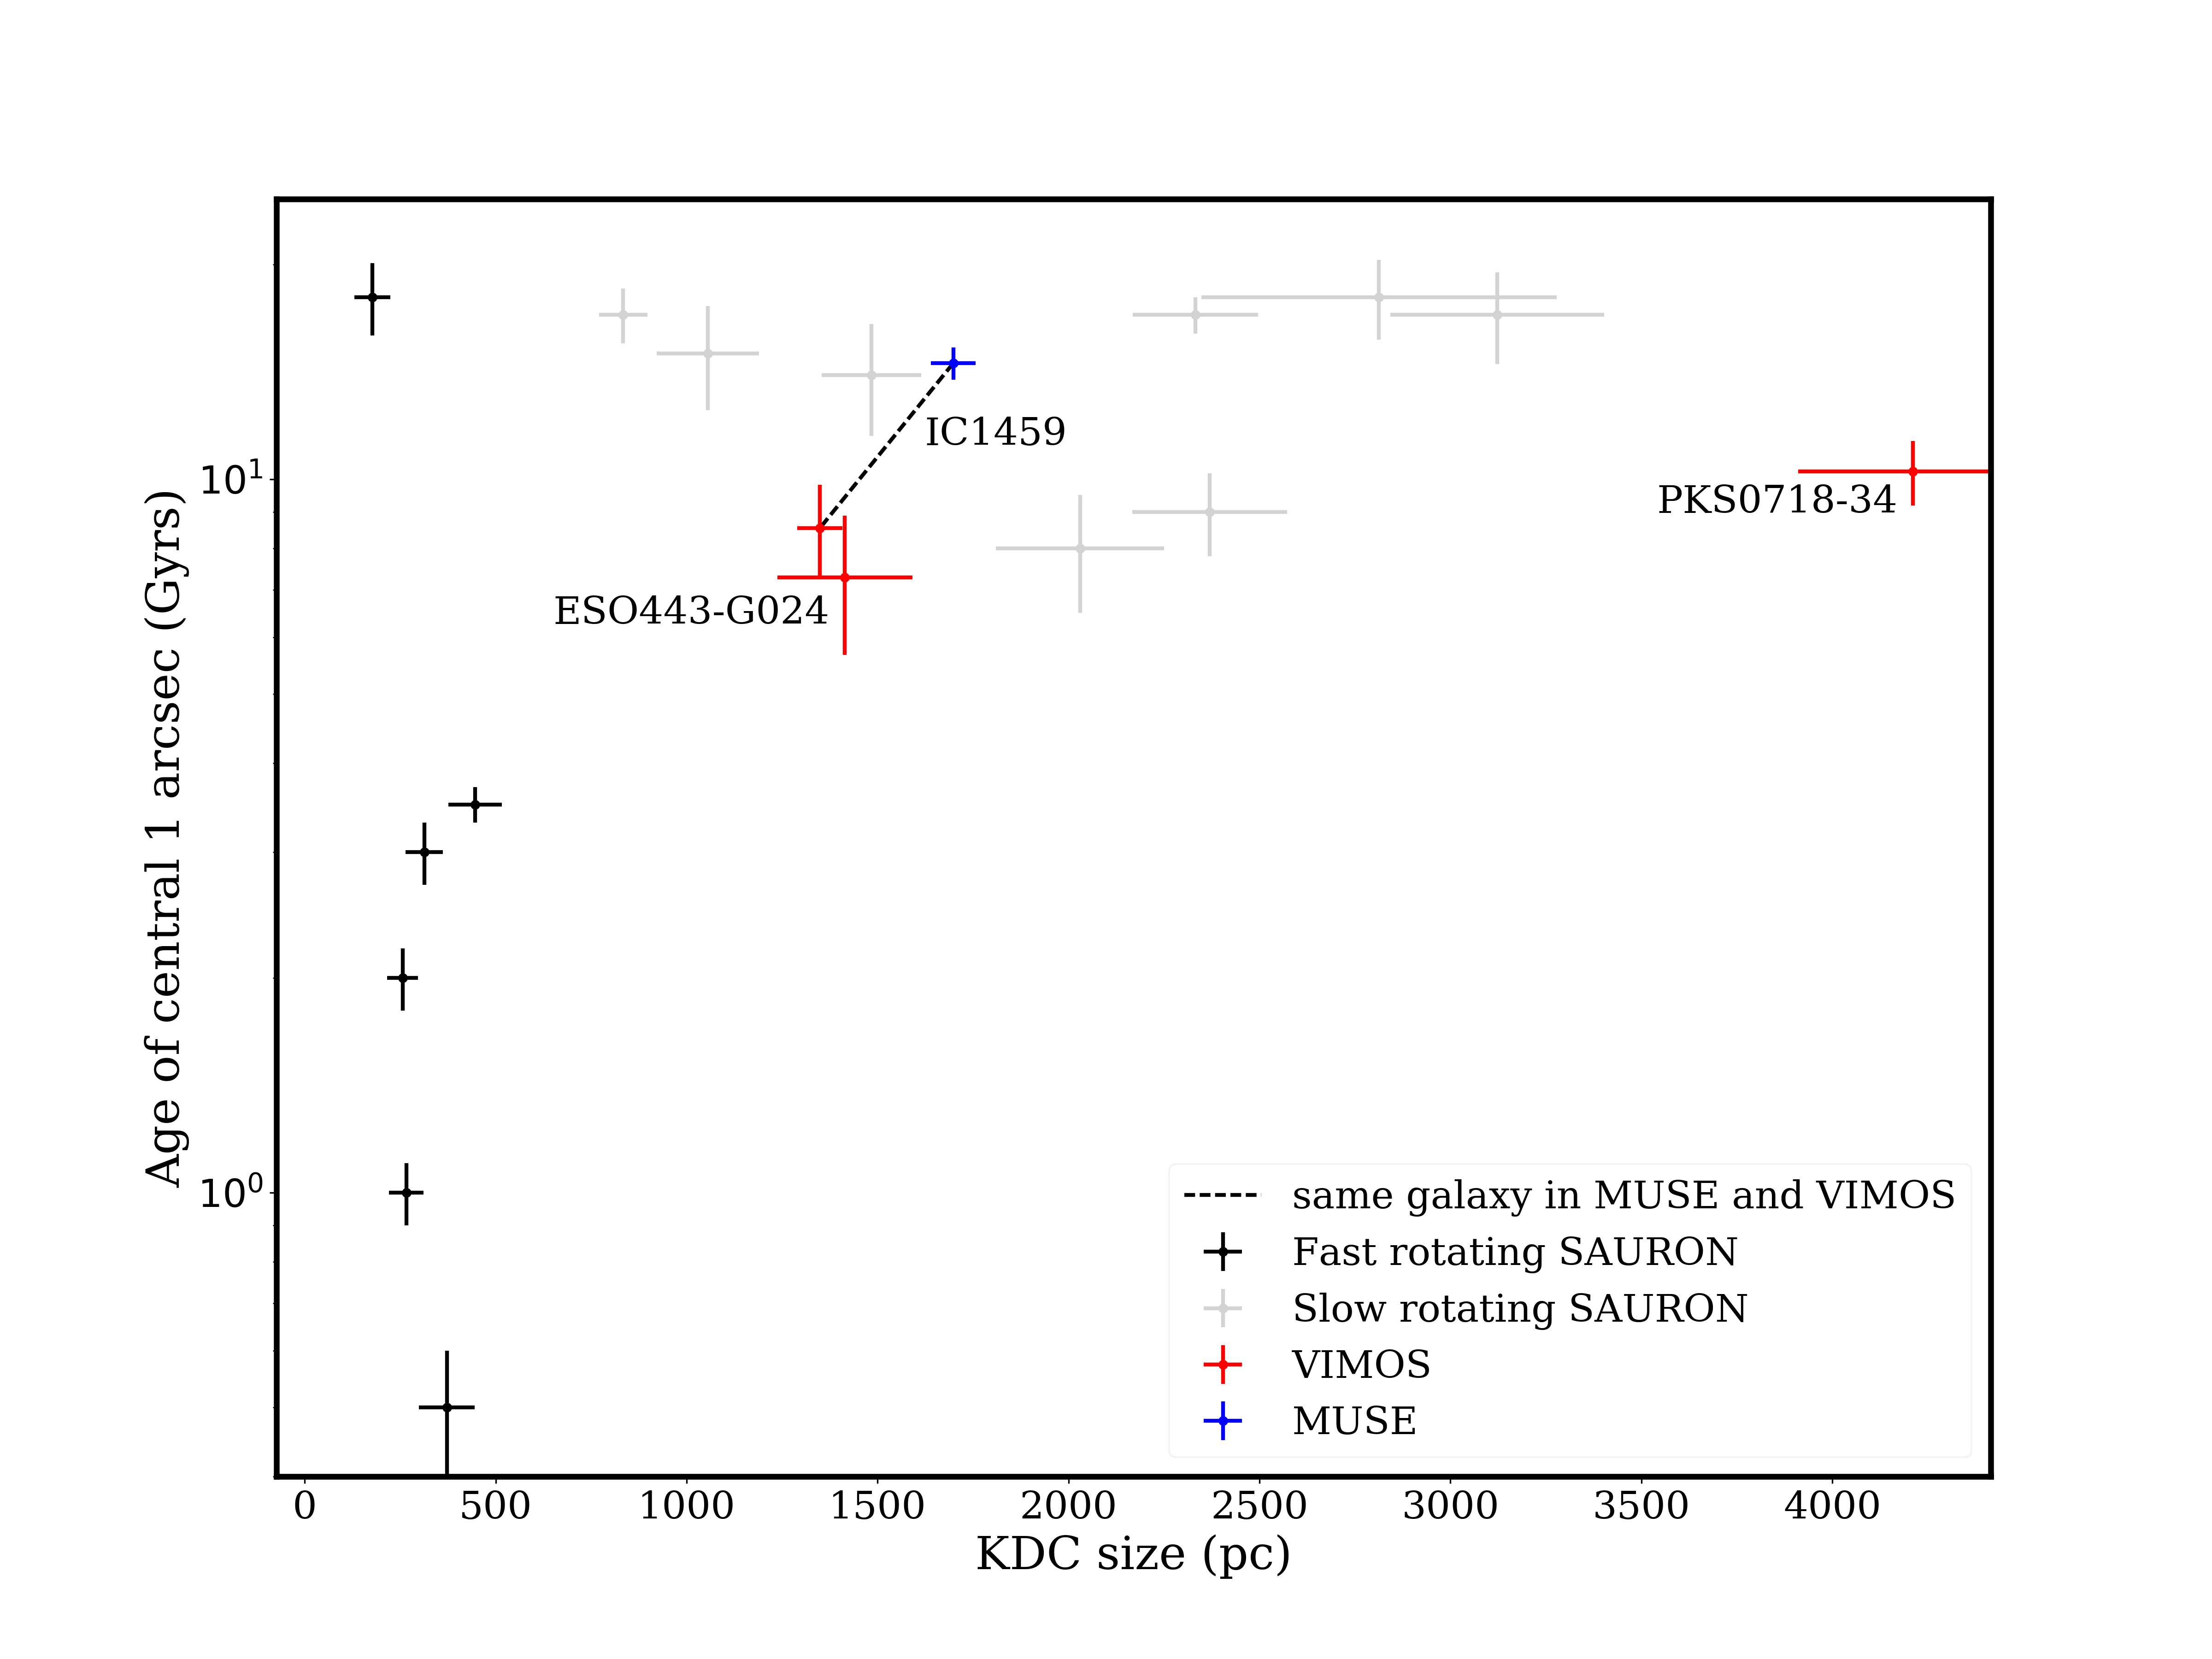
\includegraphics[width=.7\textwidth]{chapter4/KDC_size_age.png}
			\caption[KDC dichotomy]{The KDC size -- age relation. KDCs exist in two classes: old or small. VIMOS is in red, MUSE in blue and SAURON from \citet{Kuntschner2010} in black and gray for fast and slow rotators respectively.}
			\label{fig:KDC}
		\end{figure}
	
\section{The case of NGC 612}
	\label{sec:NGC612}

	Most of the galaxies in our Southern sample show typical ETG behavior: old, metal rich stellar populations with high stellar velocity dispersions with the exception of NGC 612. This galaxy has very high rotational velocities for an ETG, with an extended CO disc and a younger stellar population. All this suggests that NGC 612 may have a very different history to the rest of the Southern Sample. We have shown that it joins the list of only a handful of known examples of disc-dominated radio (AGN) galaxies \citep[e.g.][]{Morganti2011}. Spiral hosts are even rarer with only 4 known cases \citep{Ledlow1998, Hota2011a, Bagchi2014, Mao2015}, though they might much more difficult to detect against the background radio emission from star formation within the spiral.

	With the dust lane obscuring much of the galaxy (including its very centre) it is difficult to observed trends within the galaxy. However, the absorption line maps (other than H\,$\beta$) appear to be misaligned with the surface brightness (see Fig.\,\ref{fig:VIMOS_absorption}). The peak of the absorption line strength maps, usually at the centre of the galaxy, is instead found to the west of the peak surface brightness. The centre of the galaxy is assumed to be to the east of the peak surface brightness. Further study at higher spatial resolutions may resolve significant substructure to this galaxy. For the time being, it is clear that this galaxy is in a class of its own within our Southern sample. 
